\documentclass[11pt, english, fleqn, DIV=15, headinclude, BCOR=2cm]{scrreprt}

\usepackage[
    color,
    bibatend,
]{../../header}

\graphicspath{{./}{../Figures/}}

\newcommand\MZ{M_{\mathrm Z^0}}
\newcommand\electron{\mathrm e^-}
\newcommand\positron{\mathrm e^+}

\usepackage{needspace}

\usepackage{mathtools}
\usepackage{listings}

\lstset{
    basicstyle=\small\ttfamily,
}

\hypersetup{
    pdftitle=
}

\usepackage{longtable}
\usepackage{subcaption}

\usepackage[all]{nowidow}

\subject{Lab report}
\title{Analysis of $Z_0$ decays}
\subtitle{Experiment E213 -- Universität Bonn}
\author{%
    Martin Ueding \\
    \small{\href{mailto:mu@martin-ueding.de}{mu@martin-ueding.de}}
    \and
    Lino Lemmer \\
    \small{\href{mailto:l2@uni-bonn.de}{l2@uni-bonn.de}}
}

\date{2016-03-02}

\publishers{Tutor: David Hohn}

\begin{document}

\maketitle

\begin{abstract}
    In this experiment we analyse data from electron positron collisions
    collected with the \textsc{opal} detector at the \textsc{lep} collider.
    Aim of the experiment is to have an insight in methods of data analysis in
    high energy physics.
    
    In the first part we learn to distinguish between the different decay
    channels of the $\mathrm{Z}^0$ boson by their signature in the detector
    with a small data sample.

    In the second part we want to find mass, decay width and partial cross
    section of the $\mathrm{Z}^0$ for different decay channels and the weak
    mixing angle angle from the forward backward asymmetry of the
    $\electron\positron \to \muup^-\muup^+$ reaction. We also want to verify
    the lepton universality and to identify the number of neutrino generations.
    For this part we use preselected data and Monte Carlo events as help.
\end{abstract}

\tableofcontents

\chapter*{Permission to upload}

I, Martin Ueding, would like to scan and upload this lab report with your
corrections to my website \href{http://martin-ueding.de}{martin-ueding.de}.
There, the original lab report as well as the reviewed one will be licensed
under the “\href{http://creativecommons.org/licenses/by-sa/4.0/}{Creative
Commons Attribution-ShareAlike 4.0 International License}”. Is that okay with
you?

Yes $\Box$ \hspace{2cm} No $\Box$

\chapter{Theory}

\section{The standard model of particle physics}

In the standard model there are generally two types of elementary particles,
fermions with spin $s = 1/2$ and bosons with spin $s = 1$. Within the fermions
there are particles which exist freely (leptons) and ones which only exist in
bound states with each other (quarks). The latter make up heavier particles
(hadrons) like the two quarks particles called mesons and baryons consisting
from three quarks. 

The leptons are three generations of particles. In every
generation one can find one charged particle with $q = -e$. These are the
electron $\mathrm e^-$, the muon $\muup^-$ and the tauon $\tauup^-$. To each
one of them there belongs a very light uncharged neutrino
$\nuup_{\mathrm{e}/\muup/\tauup}$.

Within the quarks one also can find three generations. The first generation
containes the up quark u and the down quark d. In the second one there are
charm c and strange s and in the third one one can find the top and the bottom
quark. All quarks carry charge and mass.

All these particles interact through different interaction types, gravity,
electromagnetic interaction, weak interaction and strong interaction. The first
one plays no role in particle physics. The strong interaction acts only on the
quarks and is intermediated by gluons, the first type of bosons. The
electromagnetic interaction acts only on charged particles and the weak
interaction on all fermions. 

The electroweak interaction is a combination of the latter two interaction
types. Speaking of symmetries we combine the $\mathrm{SU}(2)$ symmetry of the
weak interaction with its three interaction particles $\mathrm W^0$, $\mathrm
W^1$ and $\mathrm W^2$ with the $\mathrm U(1)$ symmetry of the electromagnetic
interaction with its particle $\mathrm B^0$ to get two charged bosons $\mathrm
W^\pm$ and two uncharged ones, $\gammaup$ and $\mathrm Z^0$, which are
superpositions of $\mathrm W^0$ and $\mathrm B^0$. The angle between the
$\gammaup$ and the $\mathrm Z^0$ in the $\mathrm W^0$-$\mathrm B^0$ plane is
called weak mixing angle. Sometimes this is also called \enquote{Weinberg
angle}, but although Weinberg did many things, this angle was introduced by
somebody else.
%TODO behave our at different distances

Since \enquote{electromagnetic calorimeter} and \enquote{hadronic calorimeter}
is quite a mouthful, we will call them \ecal{} and \hcal{} from now on.

\section{Decay channels of the $\mathrm Z^0$ boson}

Since the $\mathrm Z^0$ doesn't carry any type of charge it only decays into
fermion-antifermion pairs. Behavior and properties of possible decay products
differ. The most obvious differences are between leptonic decay and hadronic
decay.

\subsection{Leptonic decay}

The leptonic decay products, $\mathrm e^+ + \mathrm e^-$, $\muup^+ + \muup^-$
and $\tauup^+ + \tauup^-$ behave similar in the beginning. They fly apart
colinear in opposite directions. Because of their high mass the tauons decay
very quickly through different decay channels listed in
Tabular~\ref{tab:tau_decay}.  Because of the great number of neutrinos for
this decay the missing total energy is characteristic. Also up to 6 charged
tracks can be observed.

\begin{table}[htbp]
    \centering
    \begin{tabular}{lSc}
        \toprule
        Decay channel & {Probability/\si\percent} & \ncharged\ \\
        \midrule
        $\piup^-\piup^0\nuup_\tauup$ & 24.0 +- 0.6 & 1 \\
        $\mathrm e^- \bar\nuup_\mathrm{e}\nuup_\tauup$ & 17.9 +- 0.3 & 1 \\
        $\muup^- \bar\nuup_\muup\nuup_\tauup$ & 17.6 +- 0.3 & 1 \\
        $\piup^-\nuup_\tauup$ & 11.6 +- 0.4 & 1 \\
        $\piup^-\piup^-\piup^+\nuup_\tauup$ & 5.6 +- 0.7 & 3 \\
        $\piup^-\piup^-\piup^+\piup^0\nuup_\tauup$ & 4.4 +- 1.6 & 3 \\
        $\piup^-\piup^0\piup^0\piup^0\nuup_\tauup$ & 3.0 +- 2.7 & 1 \\
        \bottomrule
    \end{tabular}
    \caption{%
        Most likely decay channels of a $\tauup^-$. %TODO cite
    }
    \label{tab:tau_decay}
\end{table}

The muons are lighter than the tauons, so they won't decay fast. Hence there
will be only two charged tracks. Since they are still heavier than electrons
they interact only very little with matter so they only lose a small amount of
energy in the detector. 

Electrons are the lightest charged leptons. They lose a lot of energy in
matter due to bremsstrahlung. As this bremsstrahlung can produce another
electron positron pair the number of charged tracks doesn't have to be exactly
two.

The pair production (s-channel) isn't the only way to get an electron positron
pair. Elastic $\mathrm e^+ + \mathrm e^-$ scattering, so called Bhabha
scattering or t-channel scattering, is for small scattering angles the
dominant process and has to be calculated out to get only decay products of
$\mathrm Z^0$.

The last leptonic decay is the neutrino pair production. Since they only
interact weak with matter they most likely will not be detected.

\subsection{Hadronic decay}

The most obvious difference of hadronic decay compared to leptonic decay is
the fact, that quarks also interact through the strong interaction.

After the quark antiquark pair is produced, the particles fly as the leptons
in opposite directions. Since the strong potential grows with distance at one
point it is energetic favourable to produce another quark antiquark pair. This
happens more than once so that it will produce a whole bunch of quarks and
antiquarks which result mostly in mesons. So there will be a lot of charged
tracks in the detector.

\section{The OPAL detector}

\section{Analysis methods}

\subsection{GROPE}

\subsection{Slice optimizing with Monte Carlo simulation}

\chapter{Exercises}

There are a couple of exercises that are supposed to be done before the
experiment.

\section{Decay width}

We are to compute the decay width~$\Gamma$ of a $\mathrm Z^0$ particle into a
pair of various fermions. The top-quark is heavier than the gauge boson,
therefore it cannot decay into a pair of top-quarks. The Feynman diagram
corresponding to the decay is shown in Figure~\ref{fig:z0-decay}.

\begin{figure}
    \centering
    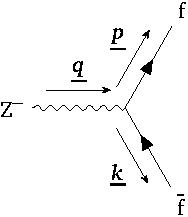
\includegraphics{z0-decay}
    \caption{%
        Decay of a $\mathrm Z^0$ gauge boson into a pair of fermions. Time is
        to the right.
    }
    \label{fig:z0-decay}
\end{figure}

First we compute the invariant matrix element~$\mathcal M$. Reading off the
Feynman diagram, we have
\begin{align*}
    \iup \mathcal M
    &= \epsilon^\mu \bar u^s(\four p) \frac{\iup g}{\cos(\theta_\text w)}
    \mat\gamma_\mu \del{g_\text v^f - g_\text a^f \mat\gamma_5} v^{s'}(\four k)
    \,,
    \intertext{%
        where we have used the rules given by \textcite[(D.56)]{romao/aqt}. We
        chose the center of mass system, as we always can for a single massive
        particle, and have $\four q = (\sqrt s, \vec 0)$. As the gauge boson
        does not have any three momentum direction, we can choose the
        polarization vector $\four \epsilon$ like we want. We chose it in the
        positive $x^3$-direction and have $\four \epsilon = (0, 0, 0, 1)$. With
        that we can simplify the Lorentz structure a little bit and obtain
    }
    &= \bar u^s(\four p) \frac{\iup g}{\cos(\theta_\text w)}
    \mat\gamma_3 \del{g_\text v^f - g_\text a^f \mat\gamma_5} v^{s'}(\four k)
    \,.
\end{align*}

For the decay width, which we are interested in, we need the modulus squared of
the matrix element. For that we need the following:
\begin{multline*}
    \sbr{\bar u^s(\four p) \mat\gamma_3 \del{g_\text v^f - g_\text a^f \mat\gamma_5}
    v^{s'}(\four k)}^\dagger \\
    =
    v^{s'}(\four k)^\dagger
    \del{g_\text v^f - g_\text a^f \mat\gamma_5^\dagger}
    \mat\gamma_3^\dagger
    \mat\gamma_0
    u^s(\four p) \\
    =
    \underbracket{v^{s'}(\four k)^\dagger
    \mat\gamma_0}
    \underbracket{\mat\gamma_0
        \del{g_\text v^f - g_\text a^f \mat\gamma_5^\dagger}
    \mat\gamma_0}
    \underbracket{\mat\gamma_0
        \mat\gamma_3^\dagger
    \mat\gamma_0}
    u^s(\four p) \\
    = \bar v^{s'}(\four k)
    \del{g_\text v^f + g_\text a^f \mat\gamma_5}
    \mat\gamma_3
    u^s(\four p) \\
    = \bar v^{s'}(\four k)
    \mat\gamma_3
    \del{g_\text v^f - g_\text a^f \mat\gamma_5}
    u^s(\four p) \,. \\
\end{multline*}

Now we can write the modulus squared of the matrix element
\begin{align*}
    |\mathcal M|^2
    &= \frac{g^2}{\cos(\theta_\text w)^2}
    \bar v^{s'}(\four k)
    \mat\gamma_3
    \del{g_\text v^f - g_\text a^f \mat\gamma_5}
    u^s(\four p)
    \bar u^s(\four p)
    \mat\gamma_3
    \del{g_\text v^f - g_\text a^f \mat\gamma_5}
    v^{s'}(\four k)
    \,. \\
    \intertext{%
        As the detector is not sensitive to the spin of the resulting fermions,
        we need to sum over all the final state spin configurations $s$ and
        $s'$. This will give us a fermion trace,
    }
    \sum_\text{spins} |\mathcal M|^2
    &=
    \frac{g^2}{\cos(\theta_\text w)^2}
    \tr\del{
        \four k
        \mat\gamma_3
        \del{g_\text v^f - g_\text a^f \mat\gamma_5}
        \four p
        \mat\gamma_3
        \del{g_\text v^f - g_\text a^f \mat\gamma_5}
    }
    \,, \\
    \intertext{%
        where we have neglected the masses of the fermions. The second
        parentheses with $\mat\gamma_5$ can be anticommuted twice and be
        collapsed with the first one. We have
    }
    &=
    \frac{g^2}{\cos(\theta_\text w)^2}
    \tr\del{
        \four k
        \mat\gamma_3
        \del{g_\text v^f - g_\text a^f \mat\gamma_5}^2
        \four p
        \mat\gamma_3
    }
    \,, \\
    \intertext{%
        where we can now simplify this. As an aside, we have
        \[
            \del{g_\text v^f - g_\text a^f \mat\gamma_5}^2
            = (g_\text v^f)^2 - (g_\text a^f)^2 - 2 g_\text v^f g_\text a^f
            \mat\gamma_5 \,.
        \]
        The square of $\mat\gamma_5$ is just the unit matrix in Dirac space.
        The term with $\mat\gamma_5$ will drop out as the trace identity
        contains the Levi-Civita symbol~$\epsilon_{\mu\nu\rho\gamma}$ which
        will be zero if two of the indices are 3, as we have in our case.
        Therefore we can directly drop that term. As it does not contain any
        further Dirac structure, we can pull it out front and obtain
    }
    &=
    \frac{g^2}{\cos(\theta_\text w)^2}
    \del{(g_\text v^f)^2 - (g_\text a^f)^2}
    \tr\del{
        \four k
        \mat\gamma_3
        \four p
        \mat\gamma_3
    }
    \,.
    \intertext{%
        Using a trace identity like given by \textcite[(A.27)]{Peskin/QFT/1995}
        we obtain
    }
    &= \frac{4 g^2}{\cos(\theta_\text w)^2} \del{(g_\text v^f)^2 - (g_\text a^f)^2}
    (2 k_3 p_3 + \four k \cdot \four p) \,.
\end{align*}
This is our final form of the matrix element.

The decay width is given by additional factors and a integration over phase
space. We have
\begin{align*}
    \Gamma_f
    &= \frac{1}{2 M_{\mathrm Z^0}} (2 \piup)^4 \int
    \frac{\dif^3 p}{(2\piup)^3 2 E_{\vec p}}
    \frac{\dif^3 k}{(2\piup)^3 2 E_{\vec k}}
    \delta^4(\four q - \four k - \four p)
    |\mathcal M|^2 \,.
    \intertext{%
        We simplify the factors and insert the matrix element and get
    }
    &= \frac{1}{32 \piup^2 M_{\mathrm Z^0}} \int
    \frac{\dif^3 p}{E_{\vec p}}
    \frac{\dif^3 k}{E_{\vec k}}
    \delta^4(\four q - \four k - \four p)
    \frac{4 g^2}{\cos(\theta_\text w)^2}
    \del{(g_\text v^f)^2 - (g_\text a^f)^2}
    (2 k_3 p_3 + \four k \cdot \four p) \,.
    \intertext{%
        Then we simplify even more and obtain
    }
    &= \frac{1}{8 \piup^2 M_{\mathrm Z^0}}
    \frac{g^2}{\cos(\theta_\text w)^2}
    \del{(g_\text v^f)^2 - (g_\text a^f)^2}
    \int
    \frac{\dif^3 p}{E_{\vec p}}
    \frac{\dif^3 k}{E_{\vec k}}
    \delta^4(\four q - \four k - \four p)
    (2 k_3 p_3 + \four k \cdot \four p) \,.
    \intertext{%
        The total energy-momentum conserving Dirac-distribution can be split
        into time-like and space-like part. In the center-of-mass frame, this
        gives us
    }
    &= \frac{1}{8 \piup^2 M_{\mathrm Z^0}}
    \frac{g^2}{\cos(\theta_\text w)^2}
    \del{(g_\text v^f)^2 - (g_\text a^f)^2}
    \\&\qquad\times
    \int
    \frac{\dif^3 p}{E_{\vec p}}
    \frac{\dif^3 k}{E_{\vec k}}
    \delta(\sqrt s - E_{\four k} - E_{\four p})
    \delta^3(\vec k + \vec p)
    (2 k_3 p_3 + \four k \cdot \four p) \,,
    \intertext{%
        which suggests the following change in variables:
        \[
            \vec a := \vec p + \vec k
            \eqnsep
            \vec b := \frac{\vec p - \vec k}{2} \,.
        \]
        The Jacobian of this transformation is unity. The $\delta^3(\vec k +
        \vec p)$ will become $\delta^3(\vec a)$, in the $\int \dif^3 a$
        integral, this will set $\vec a$ to $\vec 0$. So far we have
    }
    &= \frac{1}{8 \piup^2 M_{\mathrm Z^0}}
    \frac{g^2}{\cos(\theta_\text w)^2}
    \del{(g_\text v^f)^2 - (g_\text a^f)^2}
    \int
    \frac{\dif^3 b}{E_{\vec p} E_{\vec k}}
    \delta(\sqrt s - E_{\vec k} - E_{\vec p})
    (2 k_3 p_3 + \four k \cdot \four p) \,.
    \intertext{%
        Now we have to replace $k$ and $p$ with $b$. We have $\vec p = \vec b$
        and $\vec k = - \vec b$. Their magnitude is the same, which is expected
        in the center-of-mass frame in a two body decay. This simplifies the
        relations to
    }
    &= \frac{1}{8 \piup^2 M_{\mathrm Z^0}}
    \frac{g^2}{\cos(\theta_\text w)^2}
    \del{(g_\text v^f)^2 - (g_\text a^f)^2}
    \int
    \frac{\dif^3 b}{E_{\vec b}^2}
    \delta(\sqrt s - 2 E_{\vec b})
    (- 2 b_3 b_3 + E_{\vec b}^2 + \vec b \cdot \vec b) \,.
    \intertext{%
        As we have massless particles, we have $E_{\vec b} = |\vec b|$. We
        change into spherical coordinates in $\vec b$ and obtain
    }
    &= \frac{1}{4 \piup M_{\mathrm Z^0}}
    \frac{g^2}{\cos(\theta_\text w)^2}
    \del{(g_\text v^f)^2 - (g_\text a^f)^2}
    \\&\qquad\times
    \int \dif b \, b^2 \int \dif \cos(\theta) \,
    \frac{1}{b^2}
    \delta(\sqrt s - 2 b)
    (- 2 b^2 \cos(\theta)^2 + b^2 + b^2) \,,
    \intertext{%
        where we have performed $\int \dif \phi = 2 \piup$ already as we do not
        have any explicit $\phi$-dependence. The radial integration will set $b
        = \sqrt s / 2$. In our case $s = M_{\mathrm Z^0}^2$ and we have
    }
    &= \frac{M_{\mathrm Z^0}}{16 \piup}
    \frac{g^2}{\cos(\theta_\text w)^2}
    \del{(g_\text v^f)^2 - (g_\text a^f)^2}
    \int \dif \cos(\theta) \,
    (- 2 \cos(\theta)^2 + 2) \,.
    \intertext{%
        The angular integration gives $(-4/3 + 4) = 8/3$, so we get
    }
    &= \frac{M_{\mathrm Z^0}}{6 \piup}
    \frac{g^2}{\cos(\theta_\text w)^2}
    \del{(g_\text v^f)^2 - (g_\text a^f)^2} \,.
    \intertext{%
        Replacing $g^2$ with $8 M_{\mathrm W}^2 G_\text F / \sqrt 2$ (see
        Equation~(2.1) from the manual) and using $M_\mathrm W = \MZ
        \cos(\theta_\mathrm w)$ (see (2.3)), we will obtain
    }
    &= \frac{2 \sqrt 2}{3 \piup}
    G_\text F M_{\mathrm Z^0}^3
    \del{(g_\text v^f)^2 - (g_\text a^f)^2} \,.
    \intertext{%
        For quarks, we also need to sum over all the colors, which just gives
        the factor $N_\mathrm c^f$ for the given flavor $f$.
    }
    &= \frac{N_\mathrm c^f 2 \sqrt 2}{3 \piup}
    G_\text F M_{\mathrm Z^0}^3
    \del{(g_\text v^f)^2 - (g_\text a^f)^2} \,.
\end{align*}

Except for a missing factor $1/8$ up front, this is the same as
Equation~(2.12) given in the manual.

% FIXME Find the missing factors.

We can now insert the various quantum numbers of particles, insert the numbers
and obtain the decay widths. Our results are listed in
Table~\ref{tab:decay_widths}.

The Fermi coupling constant has the value \SI{<< fermi_coupling
>>}{\per\giga\electronvolt\squared}, see Equation~(2.1) in the manual.

\begin{table}
    \centering
    \begin{tabular}{lcccS}
        \toprule
        Flavor & $I_3$ & $Q$ & $N_\text c$ & $\Gamma / \si{\mega\electronvolt}$ \\
        \midrule
        Electron & $-1/2$ & $-1$ & 1 & << gamma_electron >> \\
        Neutrino & $1/2$ & $0$ & 1 & << gamma_neutrino >> \\
        Up-Quark & $1/2$ & $2/3$ & 3 & << gamma_up_type >> \\
        Down-Quark & $-1/2$ & $-1/3$ & 3 & << gamma_down_type >> \\
        \bottomrule
    \end{tabular}
    \caption{%
        Decay widths for the various families of fermions. As the fermions are
        taken to be massless, only one representative of the family is
        mentioned in the column \enquote{Flavor}.
    }
    \label{tab:decay_widths}
\end{table}

\section{Partial widths}

In the previous section, we have computed the decay widths for each kind of
particle. Now we have to group the various particles into families and add
their partial widths.

\begin{description}
    \item[Hadronic width]
        The hadrons in the final state are the up, down, strange, charm and
        bottom quarks. Therefore we have two up-type and three down-type quarks
        which results in a width of
        $\Gamma_\text{had.} = \SI{<< hadronic_width >>}{\mega\electronvolt}$.
        The branching ratio here is \num{<< hadronic_ratio >>}.

    \item[Charged leptonic width]
        The charged leptons are the electron, the myon and the tau. The charged
        leptonic width therefore is
        $\Gamma_\text{ch.lep.} = \SI{<< charged_leptonic_width >>}{\mega\electronvolt}$.
        The branching ratio here is \num{<< charged_leptonic_ratio >>}.

    \item[Neutral leptonic width]
        The neutral leptons are the electron-neutrino, the myon-neutrino and
        the tau-neutrino. The neutral
        leptonic width therefore is
        $\Gamma_\text{n.lep.} = \SI{<< neutral_leptonic_width >>}{\mega\electronvolt}$.
        The branching ratio here is \num{<< neutral_leptonic_ratio >>}.

    \item[Total width]
        Summing all those widths up, we obtain
        $\Gamma_\text{tot.} = \SI{<< total_width >>}{\mega\electronvolt}$.
\end{description}

All numerical values as well as the partial cross sections are in
Table~\ref{tab:partial_stuff}. The total cross section is
\[
    \sigma_\text{total}^\text{peak} = \frac{12 \piup}{\MZ^2} \frac{\Gamma_\text
    e}{\Gamma_{\mathrm Z^0}} \,.
\]

\begin{table}
    \centering
    \begin{tabular}{lSSS}
        \toprule
        Type & {Width / \si{\mega\electronvolt}} & {Branching ratio} & {Partial
    cross section / \SI{e-11}{\per\mega\electronvolt\squared}} \\
        \midrule
        Hadronic
        & << hadronic_width >> & << hadronic_ratio >> & <<
        hadronic_partial_cross_section >> \\
        Charged leptonic
        & << charged_leptonic_width >> & << charged_leptonic_ratio >> & <<
        charged_leptonic_partial_cross_section >> \\
        Neutral leptonic
        & << neutral_leptonic_width >> & << neutral_leptonic_ratio >> & <<
        neutral_leptonic_partial_cross_section >> \\
        Total
        & << total_width >> & 1 & <<
        total_cross_section >> \\
        \bottomrule
    \end{tabular}
    \caption{%
        Partial decay widths, branching ratios and cross sections.
    }
    \label{tab:partial_stuff}
\end{table}

\section{Additional generation}

If we have an additional generation, we have one more up-type and down-type
quark. Also one more lepton-type and another neutrino-type. Therefore we need
to add to the total width. The ratio is
\[
    \frac{\Gamma_\text{total} + \Gamma_\mathrm e + \Gamma_\nuup +
    \Gamma_\mathrm u + \Gamma_\mathrm d}{\Gamma_\text{total}}
    = 1 + \frac{\Gamma_\mathrm e + \Gamma_\nuup + \Gamma_\mathrm u +
    \Gamma_\mathrm d}{\Gamma_\text{total}}
    = \num{<< extra_width >>} \,.
\]
We see that another generation of quarks and leptons significantly changes the
total width and therefore also the total cross section.

\section{Angular dependence}

As we can see from the tree-level \textsc{qft} calculation for the $\mathrm
Z^0$ decay in the first problem, the angular dependence is indeed $(1 +
\cos(\theta)^2)$ as stated in the last paragraph on page~27 in the manual.
This is the $s$-channel. For the $t$-channel the angular dependence is $(1 -
\cos(\theta))\inv$.

The reaction $\mathrm{e^+ e^- \to \muup^+ \muup^-}$ only works in the
$s$-channel. The reaction $\mathrm{e^+ e^- \to e^+ e^-}$ works in both $s$- and
$t$-channel.

All we have to do is to plot those two simple functions. The plots are shown in
Figure~\ref{fig:channels}. As written in the manual, the $t$-channel becomes
dominant for very small angles, i.e.\ large $\cos(\theta)$.

\begin{figure}
    \centering
    \includegraphics{s-channel}
    \caption{%
        Angular dependence of differential cross section in the $s$- and
        $t$-channel.
    }
    \label{fig:channels}
\end{figure}

\section{Asymmetry}
\label{sec:exercises-asymmetry}

We are to compute the forward--backward asymmetry of the reaction $\mathrm e^+
\mathrm e^- \to \muup^+ \muup^-$. The given values for Mandelstam-$s$ are
\SIlist{<< ';'.join(s_array) >>}{\giga\electronvolt}. The values for the weak
mixing angle in terms of $\sin(\theta_\text w)^2$ given are \numlist{<<
';'.join(sin_sq_array) >>}. In total there are nine combinations, all are shown
in Table~\ref{tab:asymmetry}.

\begin{table}
    \centering
    \begin{tabular}{S*3S}
        \toprule
        & \multicolumn{3}{c}{$A_\text{FB}^\muup$} \\
        \cmidrule(l){2-4}
        {$s$}
        %< for x in sin_sq_array >%
        & {$\sin(\theta_\text w)^2 = \num{<< x >>}$}
        %< endfor >%
        \\
        \midrule
        %< for row in asymmetry_table >%
        << ' & '.join(row) >> \\
        %< endfor >%
        \bottomrule
    \end{tabular}
    \caption{%
        Forward--backward asymmetry $A_\text{FB}^\muup$ for different
        values of Mandelstam-$s$ (rows) and different values of $\theta_\text
        w$ (columns).
    }
    \label{tab:asymmetry}
\end{table}

The equation that we use is (2.19) from the manual:
\[
    A_\text{FB}^f(s) \simeq - \frac 32 \frac{a_\mathrm e a_f Q_f \Re(\chi(s))}{(v_\mathrm e^2
    + a_\mathrm e^2)(v_f^2 + a_f^2)} \,,
\]
where $\chi(s)$ is the propagator of the $\mathrm Z^0$ boson as given in
(2.11). It differs from the usual propagator of a vector particle and does not
have any Lorentz structure. This is odd, we will just use the given propagator.
The real part of that propagator has to be found by making the denominator
real:
\[
    \chi(s)
    = \frac{s}{s - \MZ^2 + \frac{\iup s \Gamma_{\mathrm Z^0}}\MZ}
    = s \frac{s - \MZ^2 - \frac{\iup s \Gamma_{\mathrm Z^0}}\MZ}
    {\del{s - \MZ^2}^2 + \del{\frac{s \Gamma_{\mathrm Z^0}}\MZ}^2} \,.
\]
The real part then is
\[
    \Re(\chi(s))
    = \frac{s(s - \MZ^2)}
    {\del{s - \MZ^2}^2 + \del{\frac{s \Gamma_{\mathrm Z^0}}\MZ}^2} \,.
\]

Now we just need to insert all the numbers with $I_3 = -1/2$ and $Q = -1$ in
both $f = \mathrm e$ and $f = \muup$.

%%%%%%%%%%%%%%%%%%%%%%%%%%%%%%%%%%%%%%%%%%%%%%%%%%%%%%%%%%%%%%%%%%%%%%%%%%%%%%%

\chapter{Analysis}

The data used in this lab experiment was gathered in the year 1992 and before.
Therefore we only do analysis of the data. Part of the analysis is done at the
university, the remainder is done at home. We will group our work by topic and
not split by university and home.

\section{Screening some decays}

At first we looked at some decays in the event display software
\textsc{grope}. In order to learn the signatures of the various decays, we
start with Monte Carlo datasets which only contain decays into a given channel.

The characteristics have different names within \textsc{grope} and
\textsc{paw}. Both are programming language identifiers and hard to
read. Since we do not want to clutter our report with those identifiers, we use
ones close to \textsc{paw} but formatted nicer. See
Table~\ref{tab:nomenclature} for an overview.

\begin{table}
    \centering
    \begin{tabular}{lll}
        \toprule
        \textsc{grope}
        & \textsc{paw}
        & Our name \\
        \midrule
        \texttt{Ctrk(N)} & \texttt{ncharged} & \ncharged\ \\
        \texttt{Ctrk(Sump)} & \texttt{pcharged} & \pcharged\ \\
        \texttt{Ecal(SumE)} & \texttt{e\_ecal} & \eecal\ \\
        \texttt{Hcal(SumE)} & \texttt{e\_hcal} & \ehcal\ \\
        \bottomrule
    \end{tabular}
    \caption{%
        Nomenclature used by \textsc{grope}, \textsc{paw} and within this lab
        report.
    }
    \label{tab:nomenclature}
\end{table}

Figure~\ref{fig:grope} shows the events as displayed by \textsc{grope}. We have
picked a representative event for each category of decay (electrons, muons,
taus, hadrons).

\begin{figure}
    \centering
    \begin{subfigure}[c]{0.48\linewidth}
        \centering
        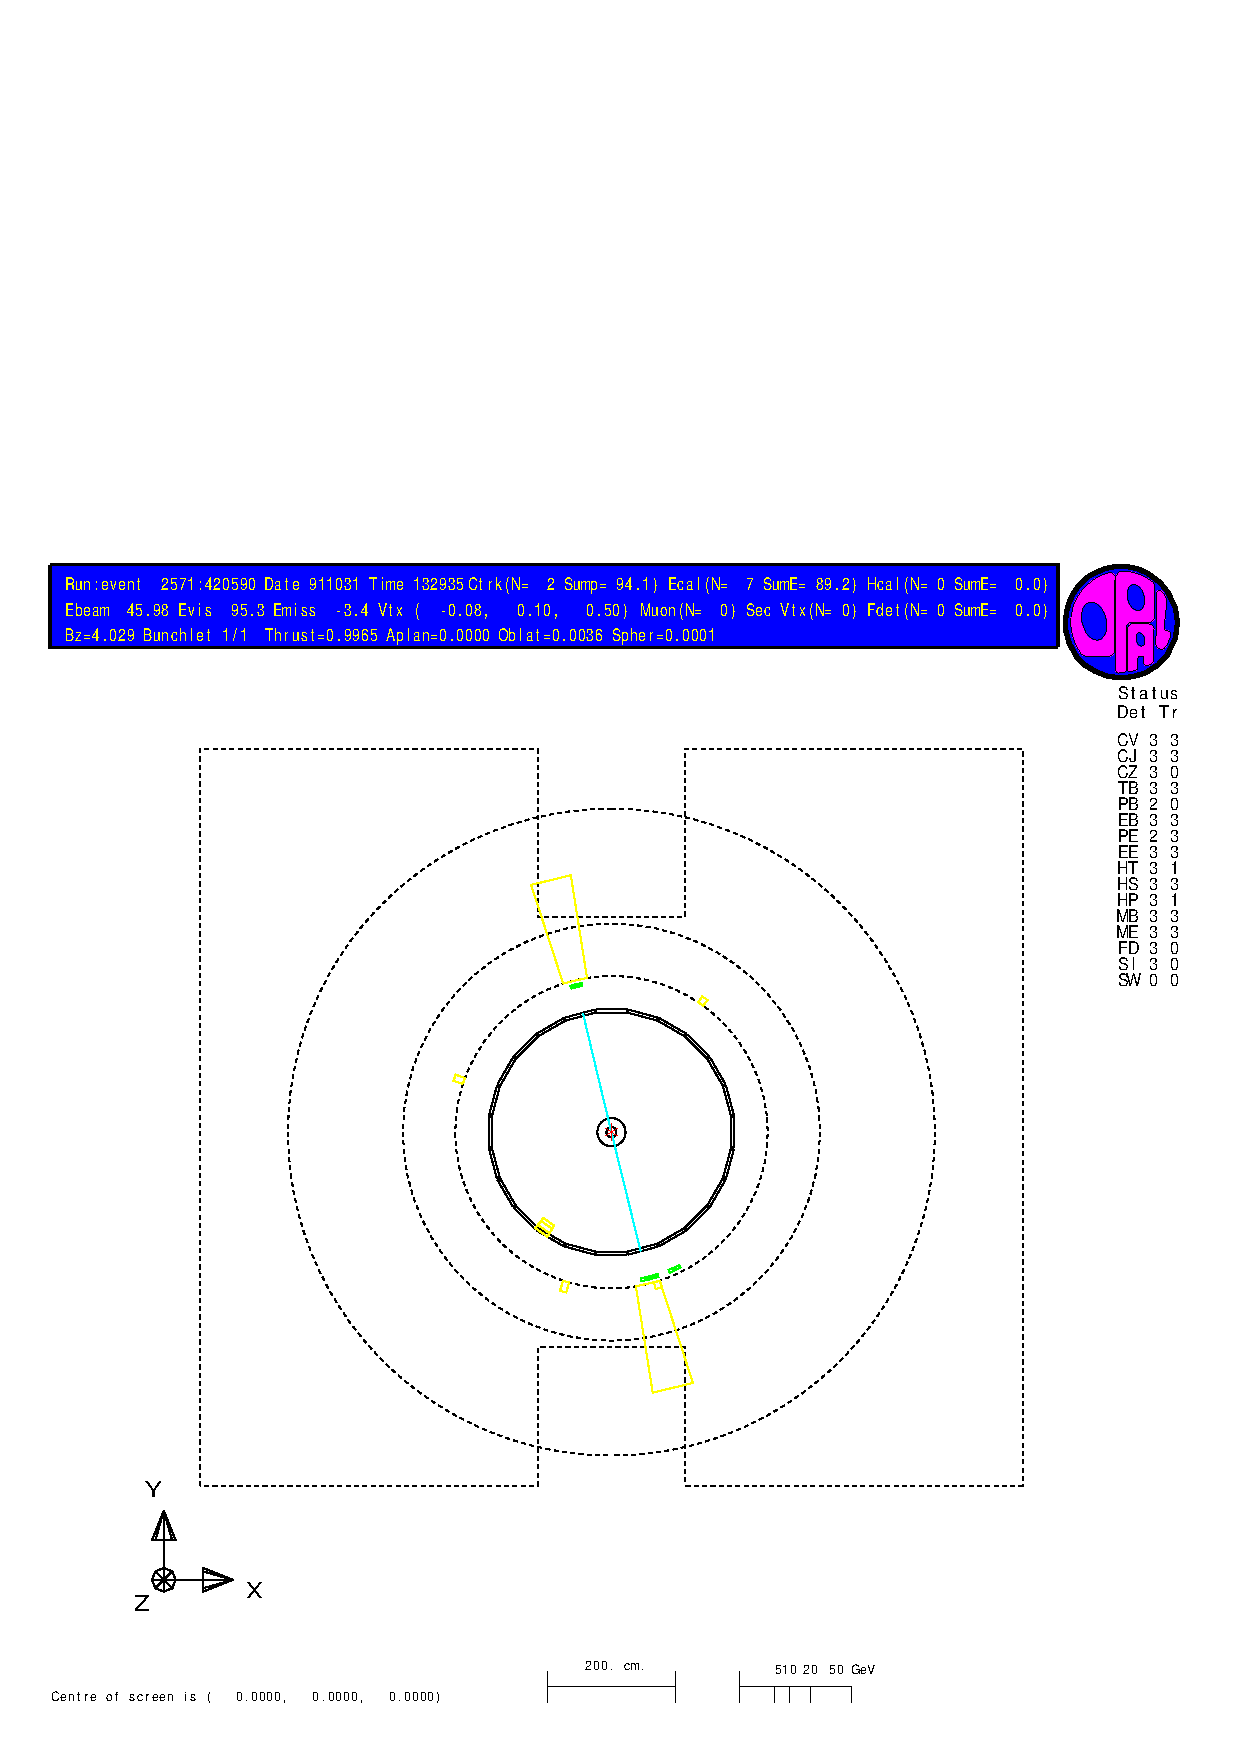
\includegraphics[width=\linewidth]{opal-electrons}
        \caption{%
            Electrons
        }
        \label{fig:grope/electrons}
    \end{subfigure}
    \hfill
    \begin{subfigure}[c]{0.48\linewidth}
        \centering
        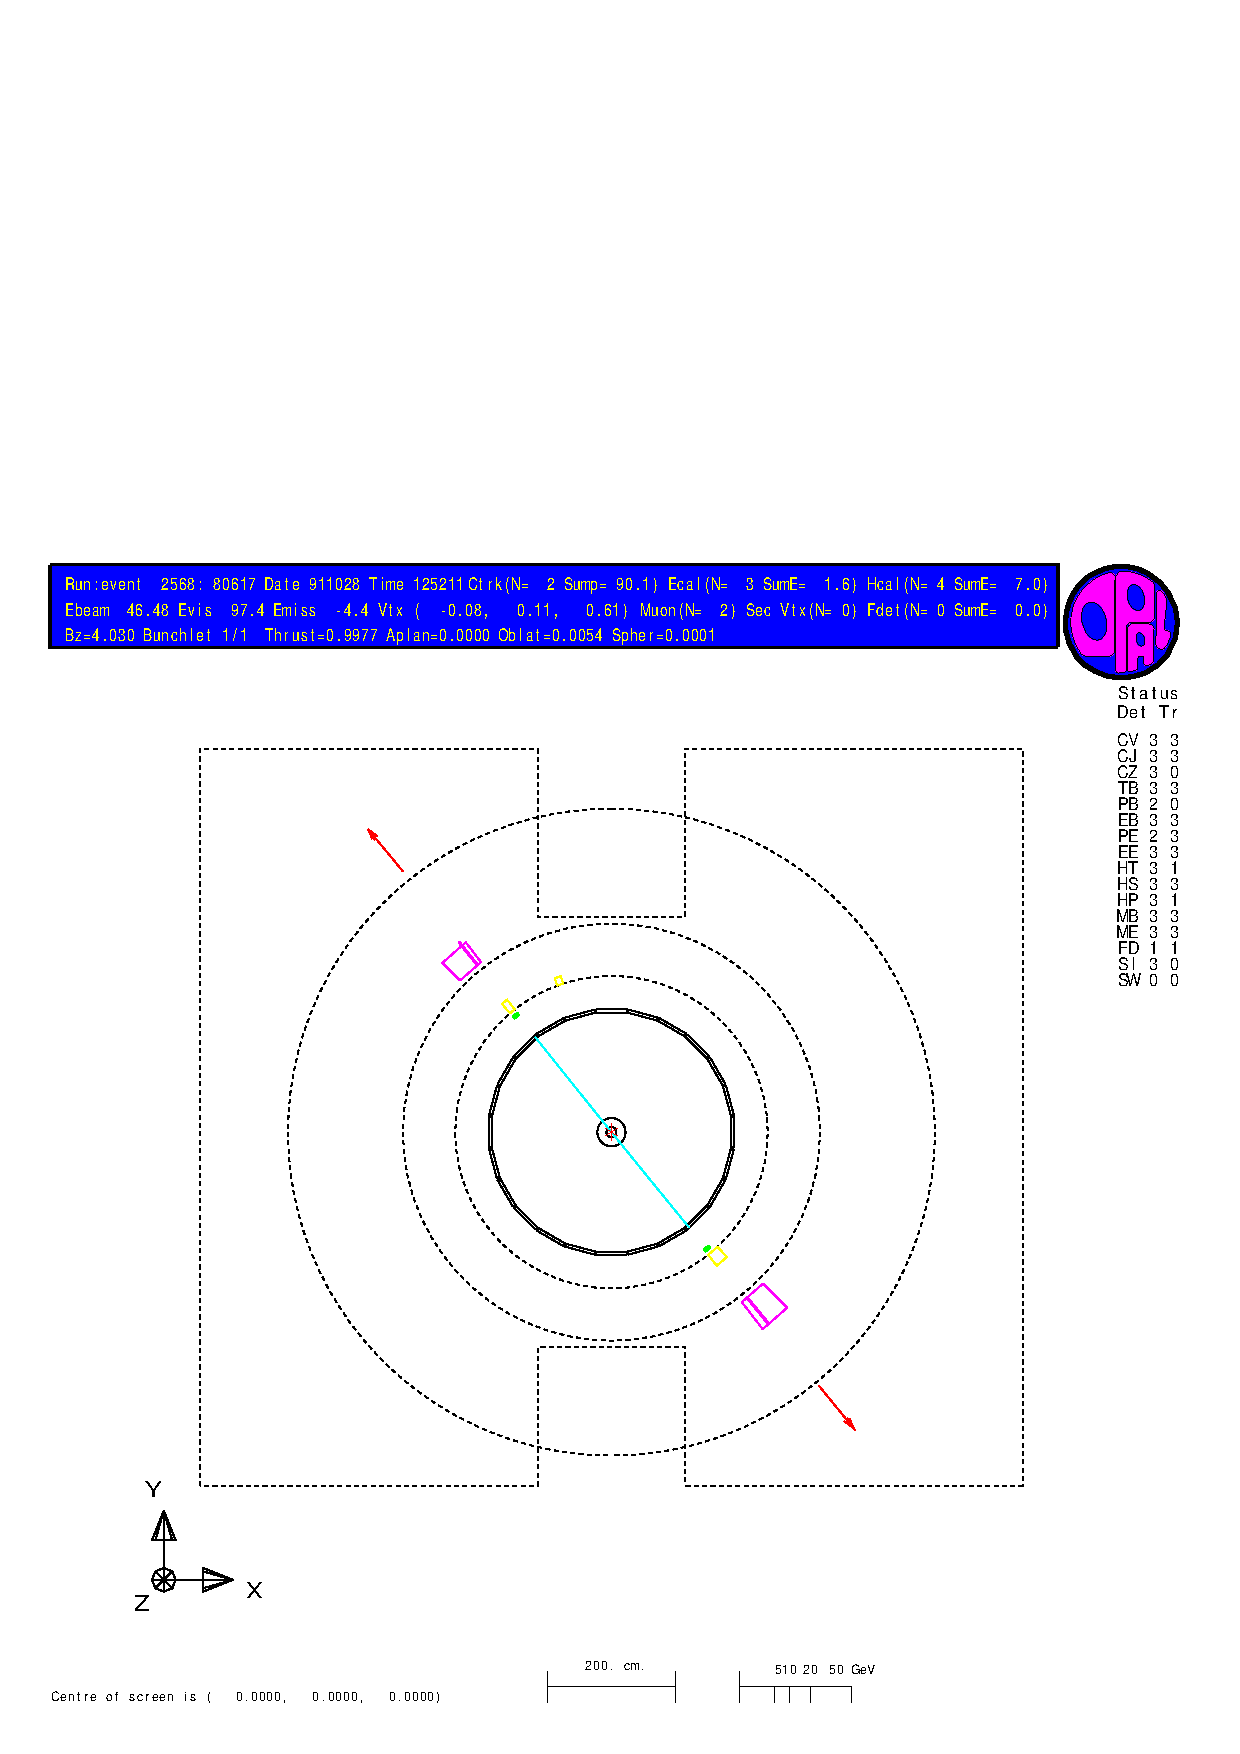
\includegraphics[width=\linewidth]{opal-muons}
        \caption{%
            Muons
        }
        \label{fig:grope/muons}
    \end{subfigure}

    \vspace{2ex}

    \begin{subfigure}[c]{0.48\linewidth}
        \centering
        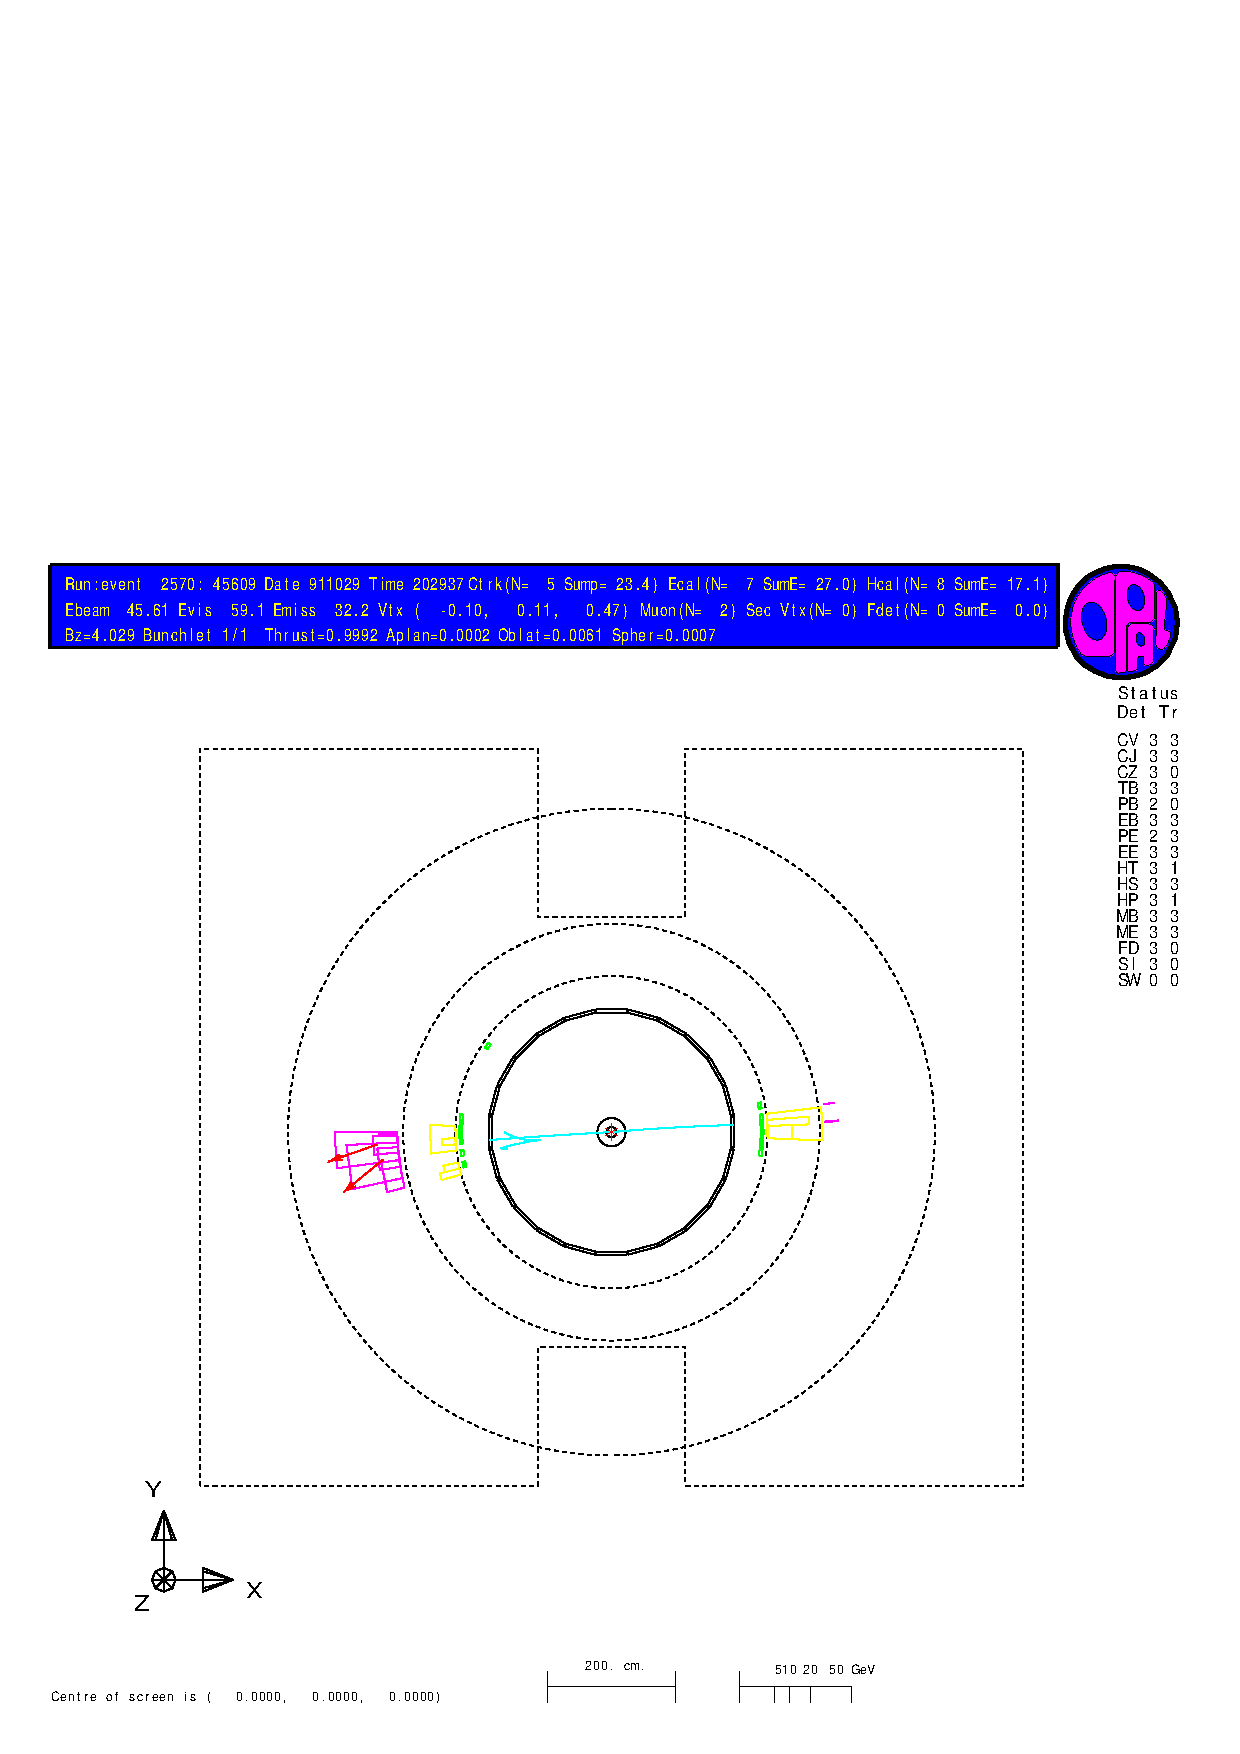
\includegraphics[width=\linewidth]{opal-taus}
        \caption{%
            Tauons
        }
        \label{fig:grope/tauons}
    \end{subfigure}
    \hfill
    \begin{subfigure}[c]{0.48\linewidth}
        \centering
        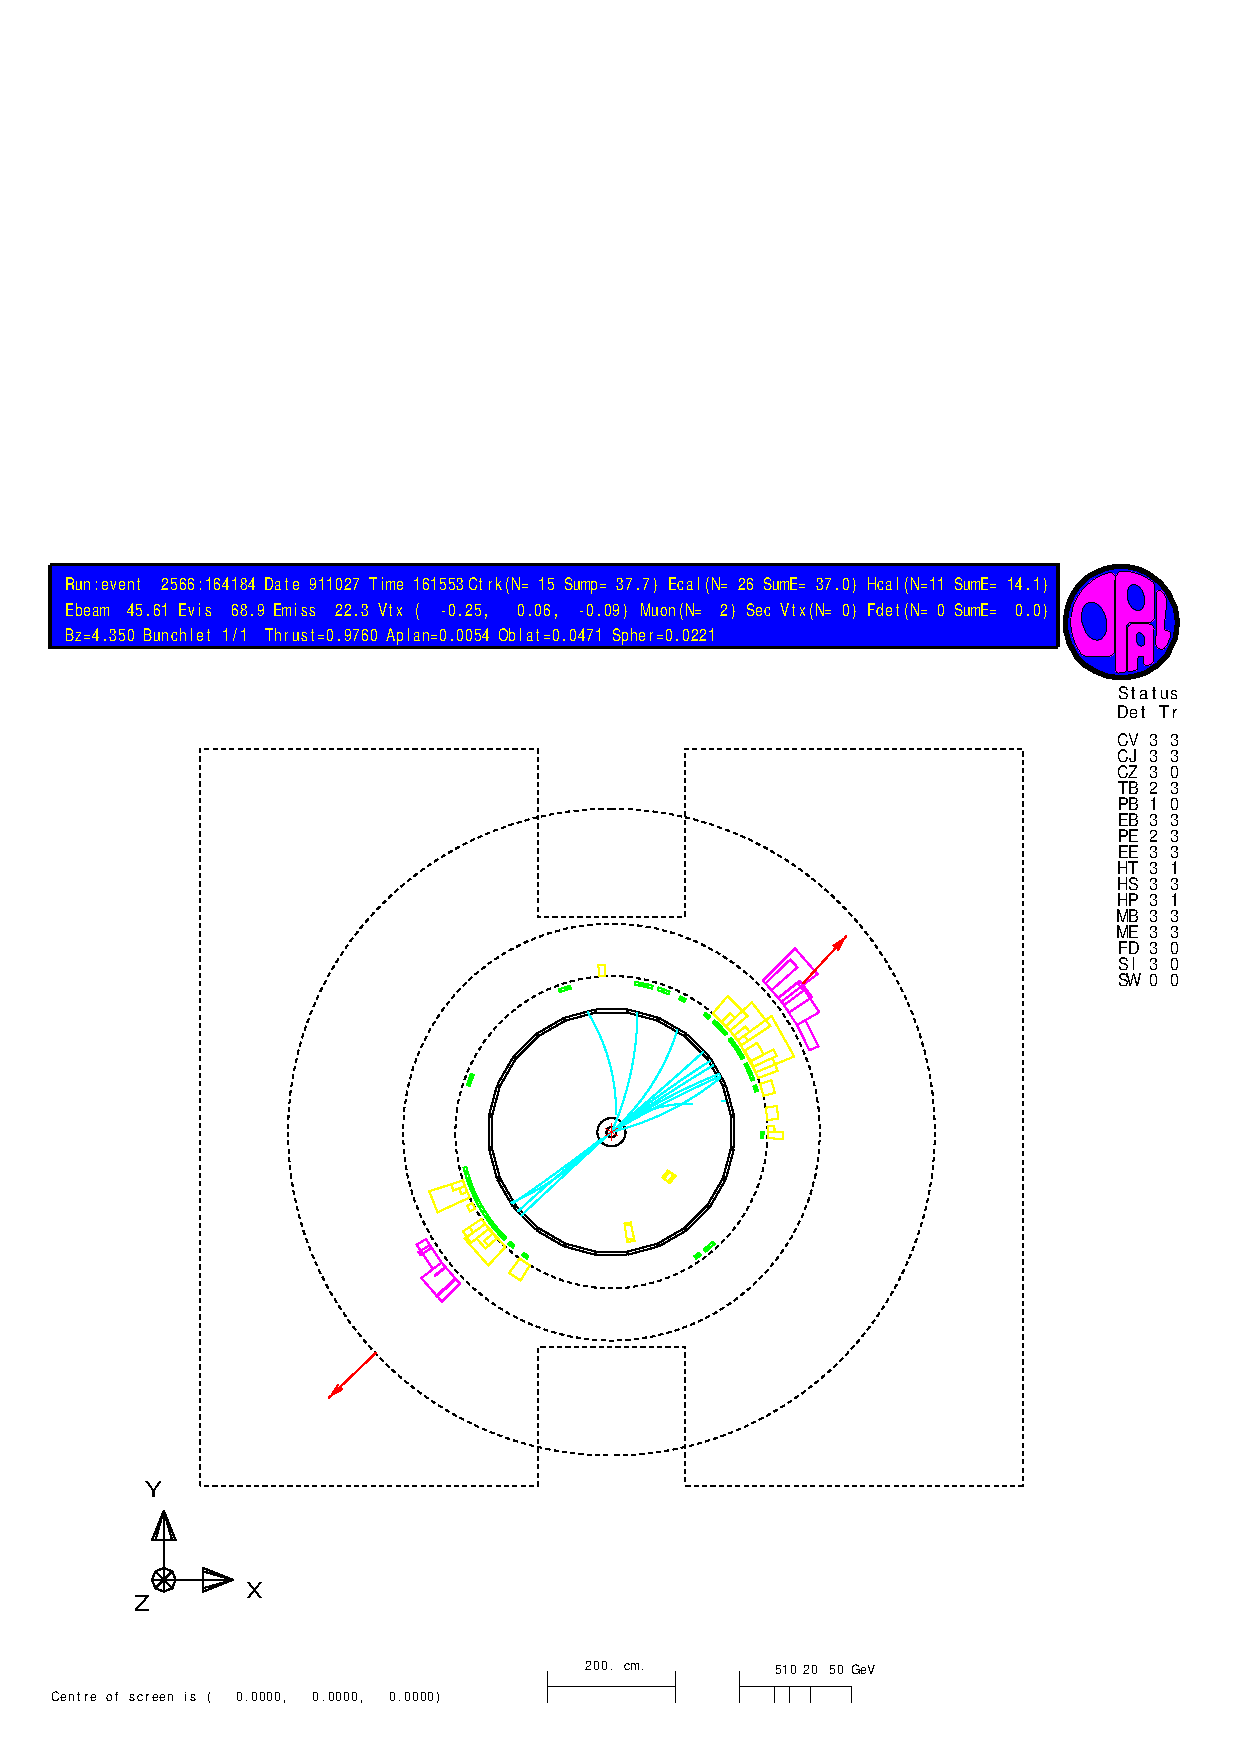
\includegraphics[width=\linewidth]{opal-hadrons}
        \caption{%
            Hadrons
        }
        \label{fig:grope/hadrons}
    \end{subfigure}
    \caption{%
        Event display of Monte Carlo events. One can see the traces from the
        vertex chamber in cyan, the hits in the \ecal{} are shown in yellow
        (probably hard to see on paper). In magenta, one has the hits in the
        \hcal{}. Muon penetrations are indicated with red arrows. Images are
        rendered with \textsc{grope}.
    }
    \label{fig:grope}
\end{figure}


The electron decay in Figure~\ref{fig:grope/electrons} shows the typical
back-to-back signature of two very fast (no curvature in the vertex chamber)
charged particles. All the energy is deposited in the \ecal{}. In the dark blue
header one can see that the missing energy is very small. The \eecal{} is
pretty much identical with \sump{}. Both energies are almost the beam energy.

Decays into muons have a different signature. The most prominent feature are
the hits in the muon chambers, as one can see in Figure~\ref{fig:grope/muons}.
The \sump{} is the beam energy, little energy is unaccounted for. This means
that there are no neutrinos created in that decay. \eecal{} and \ehcal{} is
small, this is due to the big mass of the muon (compared to electrons).

Figure~\ref{fig:grope/taus} shows a decay into taus. This decay is not as
simple as the previous ones. We have some missing energy (around a third), more
than one charged track and also energy deposited into the various calorimeters.
The missing energy comes from the neutrinos in the weak decay of the tau. The
number of charged tracks is still small (just five), therefore we can
differentiate from the hadronic decays.

Lastly, a decay into hadrons is shown in Figure~\ref{fig:grope/hadrons}. One
directly sees the large number of tracks, here 26, which exhibit a larger
curvature. Also we have nonzero \ehcal{}. Hadronic decays are easy to classify
as their number of charged tracks is always rather large.

\section{Defining the cuts}

While reviewing the Monte Carlo events in \textsc{grope}, we generate
histograms with the various characteristics. We choose to write down
\ncharged{}, \sump{}, \eecal{} and \ehcal{}. Those characteristics are also
available in the later analysis of larger datasets using \textsc{paw}.

\subsection{Preliminary analysis}

Using some twenty points per event class, we obtain the histograms shown in
Figure~\ref{fig:hist}. There one can see that some characteristics are well
suited to cut the data. For instance in \ncharged, we see that hadronic decays
have more than seven tracks, whereas the leptonic decays have less. In the
histogram for \sump, we see that a cut at around \SI{80}{\giga\electronvolt}
can separate taus and muons. Another cut in the \ecal-energy at around
\SI{75}{\giga\electronvolt} allows us to separate taus and electrons. The
energy deposited into the \hcal\ is not very helpful for cutting.

\begin{figure}
    \centering
    \begin{subfigure}[c]{0.49\linewidth}
        \centering
        \includegraphics{hist-ctrk_n}
        \caption{%
            \ncharged
        }
        \label{fig:hist/ncharged}
    \end{subfigure}
    \hfill
    \begin{subfigure}[c]{0.49\linewidth}
        \centering
        \includegraphics{hist-ctrk_sump}
        \caption{%
            \pcharged/\si{\giga\electronvolt}
        }
        \label{fig:hist/pcharged}
    \end{subfigure}

    \vspace{2ex}

    \begin{subfigure}[c]{0.49\linewidth}
        \centering
        \includegraphics{hist-ecal_sume}
        \caption{%
            \eecal/\si{\giga\electronvolt}
        }
        \label{fig:hist/eecal}
    \end{subfigure}
    \hfill
    \begin{subfigure}[c]{0.49\linewidth}
        \centering
        \includegraphics{hist-hcal_sume}
        \caption{%
            \ehcal/\si{\giga\electronvolt}
        }
        \label{fig:hist/ehcal}
    \end{subfigure}
    \caption{%
        Histograms with data gathered from Monte Carlo datasets in
        \textsc{grope}. The number of charged tracks is shown as a histogram
        with logarithmic bins.
    }
    \label{fig:hist}
\end{figure}


Having those cuts in place, we take a look at the \texttt{test} datasets which
are not sorted by event type. There we try to use our fresh intuition about the
decay channels to identify the type of decay. Then we take a look at the
characteristics and see whether our cuts would come to the same conclusion. For
most decays, this worked out well. Some were not classified correctly; this is
somewhat expected as we will never be able to avoid false-positives and
false-negatives.

While we were trying to find suitable cuts, a 3D visualization like shown in
Figure~\ref{fig:mpl-scatter} was really helpful. There we could turn the cloud
of events in the parameter space and see different clusters. Such a
3D-representation can hardly be printed and must be viewed interactively,
though.

\begin{figure}
    \centering
    \includegraphics[width=.6\linewidth]{mpl-scatter}
    \caption{%
        3D visualization of the three most expressive characteristics.
    }
    \label{fig:mpl-scatter}
\end{figure}

We would really have liked to perform this visualization with more data. Then
one could even do a 3D-histogram and find cut surfaces which separate the data
most cleanly. In \textsc{paw} we were limited to hyperplanes anyway, so we just
chose a few axis-parallel planes as they did the job sufficiently well.

After the refining, we have the cuts listed in Table~\ref{tab:cuts}.

\begin{table}
    \centering
    \begin{tabular}{lcccc}
        \toprule
        & \multicolumn{4}{c}{Cut criterion} \\
        \cmidrule(l){2-5}
        Particle
        & \ncharged
        & \sump/\si{\giga\electronvolt}
        & \eecal/\si{\giga\electronvolt}
        & \ehcal/\si{\giga\electronvolt} \\
        \midrule
        Electrons & $< 4$ &  & $> 60$ &  \\
        Muons & $< 4$ & $> 75$ & $< 20$ &  \\
        Taus & $< 7$ & $< 75$ & $\leq 75$ &  \\
        Hadrons & $> 7$ &  &  &  \\
        \bottomrule
    \end{tabular}
    \caption{%
        Cuts derived from the few data points manually extracted from the Monte
        Carlo events.
    }
    \label{tab:cuts}
\end{table}

\subsection{More data points}

Our histograms are only filled with a limited amount of data. It would be wise
to use more data to refine the cuts further. To that end, we change from
the single event viewer \textsc{grope} to the analysis tool \textsc{paw} which
is a predecessor to \textsc{root}.

We load the big Monte Carlo datasets into \textsc{paw} and let it generate
histograms with the characteristics. Sadly we only have the exported postscript
documents and not the raw data. Therefore we can only present ill-looking plots
in Figure~\ref{fig:paw-ncharged}. Although the labels are ridiculously small,
we have crammed four plots as we would have needed four pages otherwise. If we
had the raw data, we would have combined the four decay modes into a single
histogram like we have done in Figure~\ref{fig:mpl-hist} with the data we
collected manually.

\begin{figure}
    \centering
    \begin{subfigure}[c]{0.48\linewidth}
        \centering
        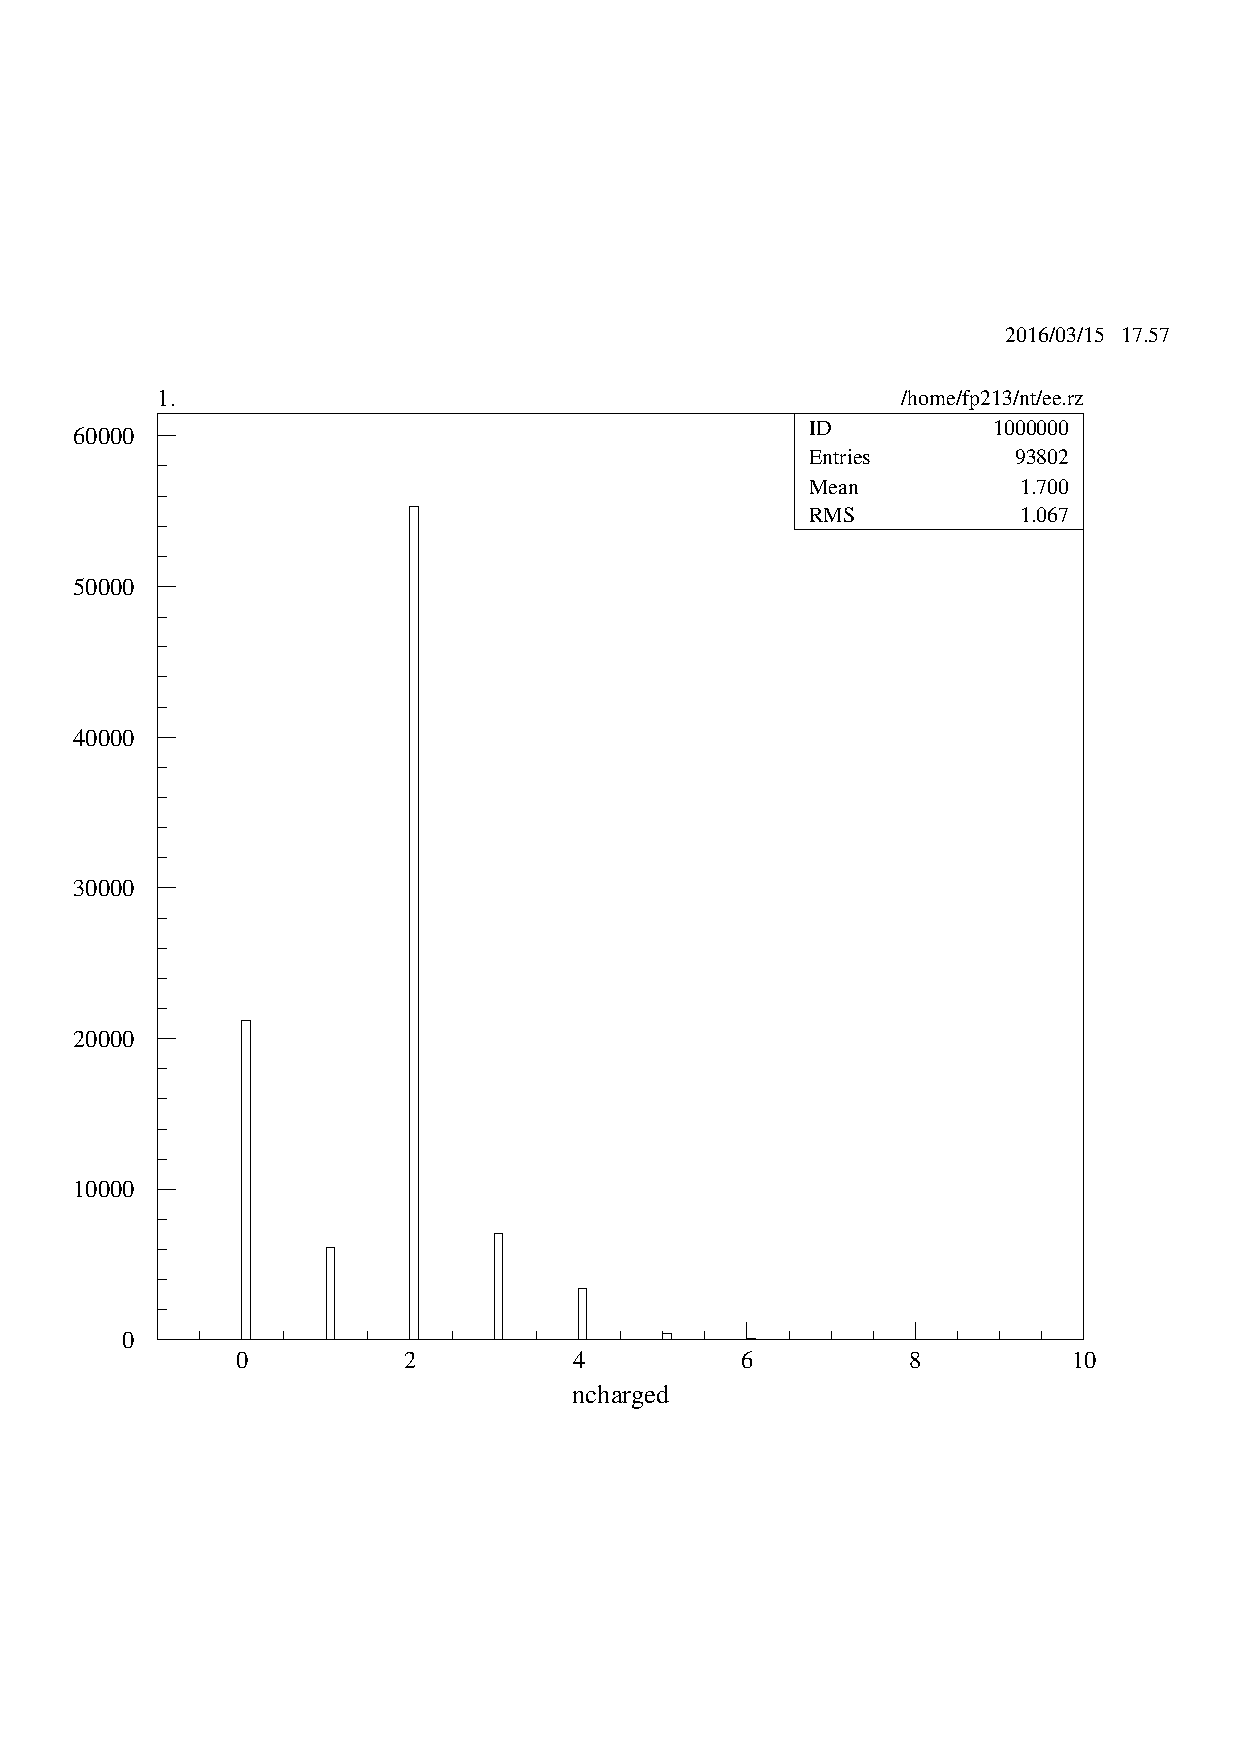
\includegraphics[width=\linewidth]{electrons-ncharged}
        \caption{%
            Electrons
        }
        \label{fig:paw-ncharged/electrons}
    \end{subfigure}
    \hfill
    \begin{subfigure}[c]{0.48\linewidth}
        \centering
        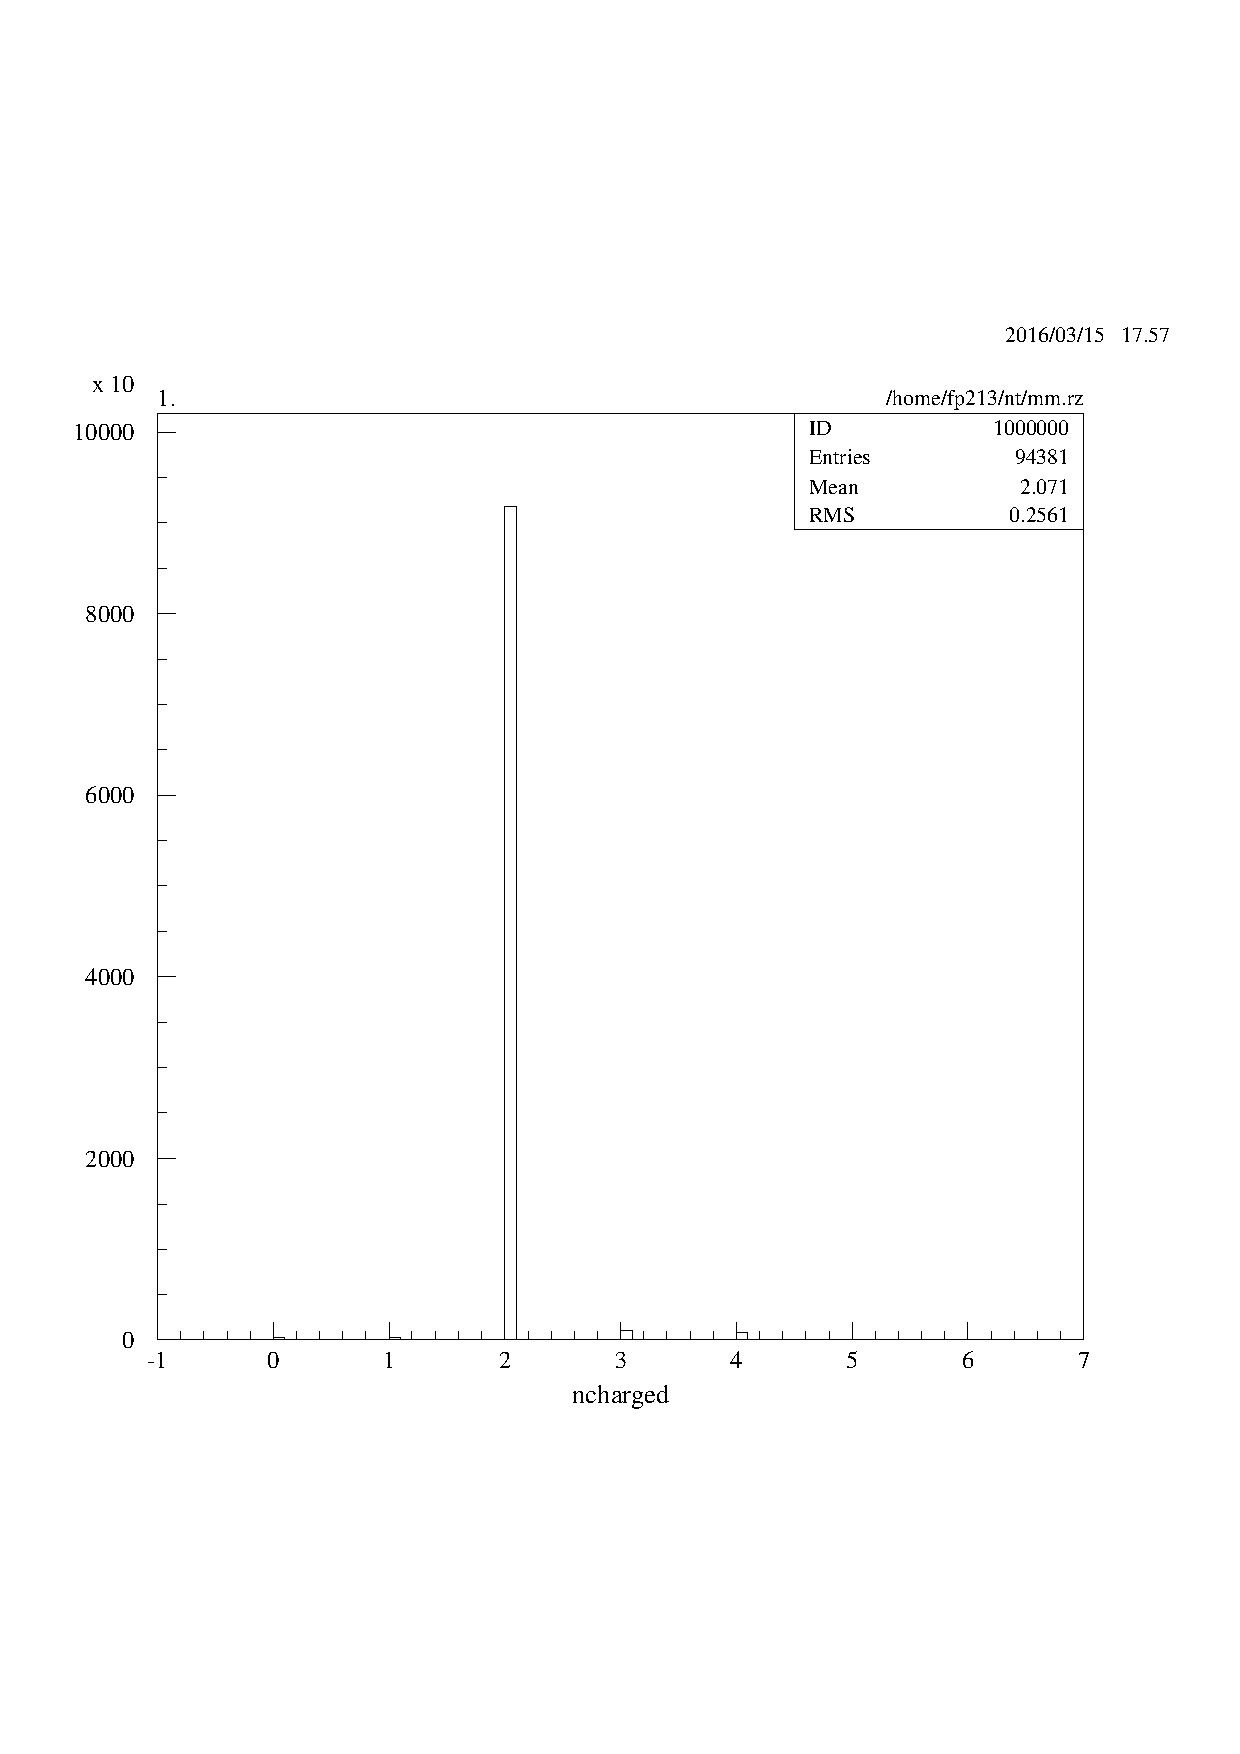
\includegraphics[width=\linewidth]{muons-ncharged}
        \caption{%
            Muons
        }
        \label{fig:paw-ncharged/muons}
    \end{subfigure}

    \vspace{2ex}

    \begin{subfigure}[c]{0.48\linewidth}
        \centering
        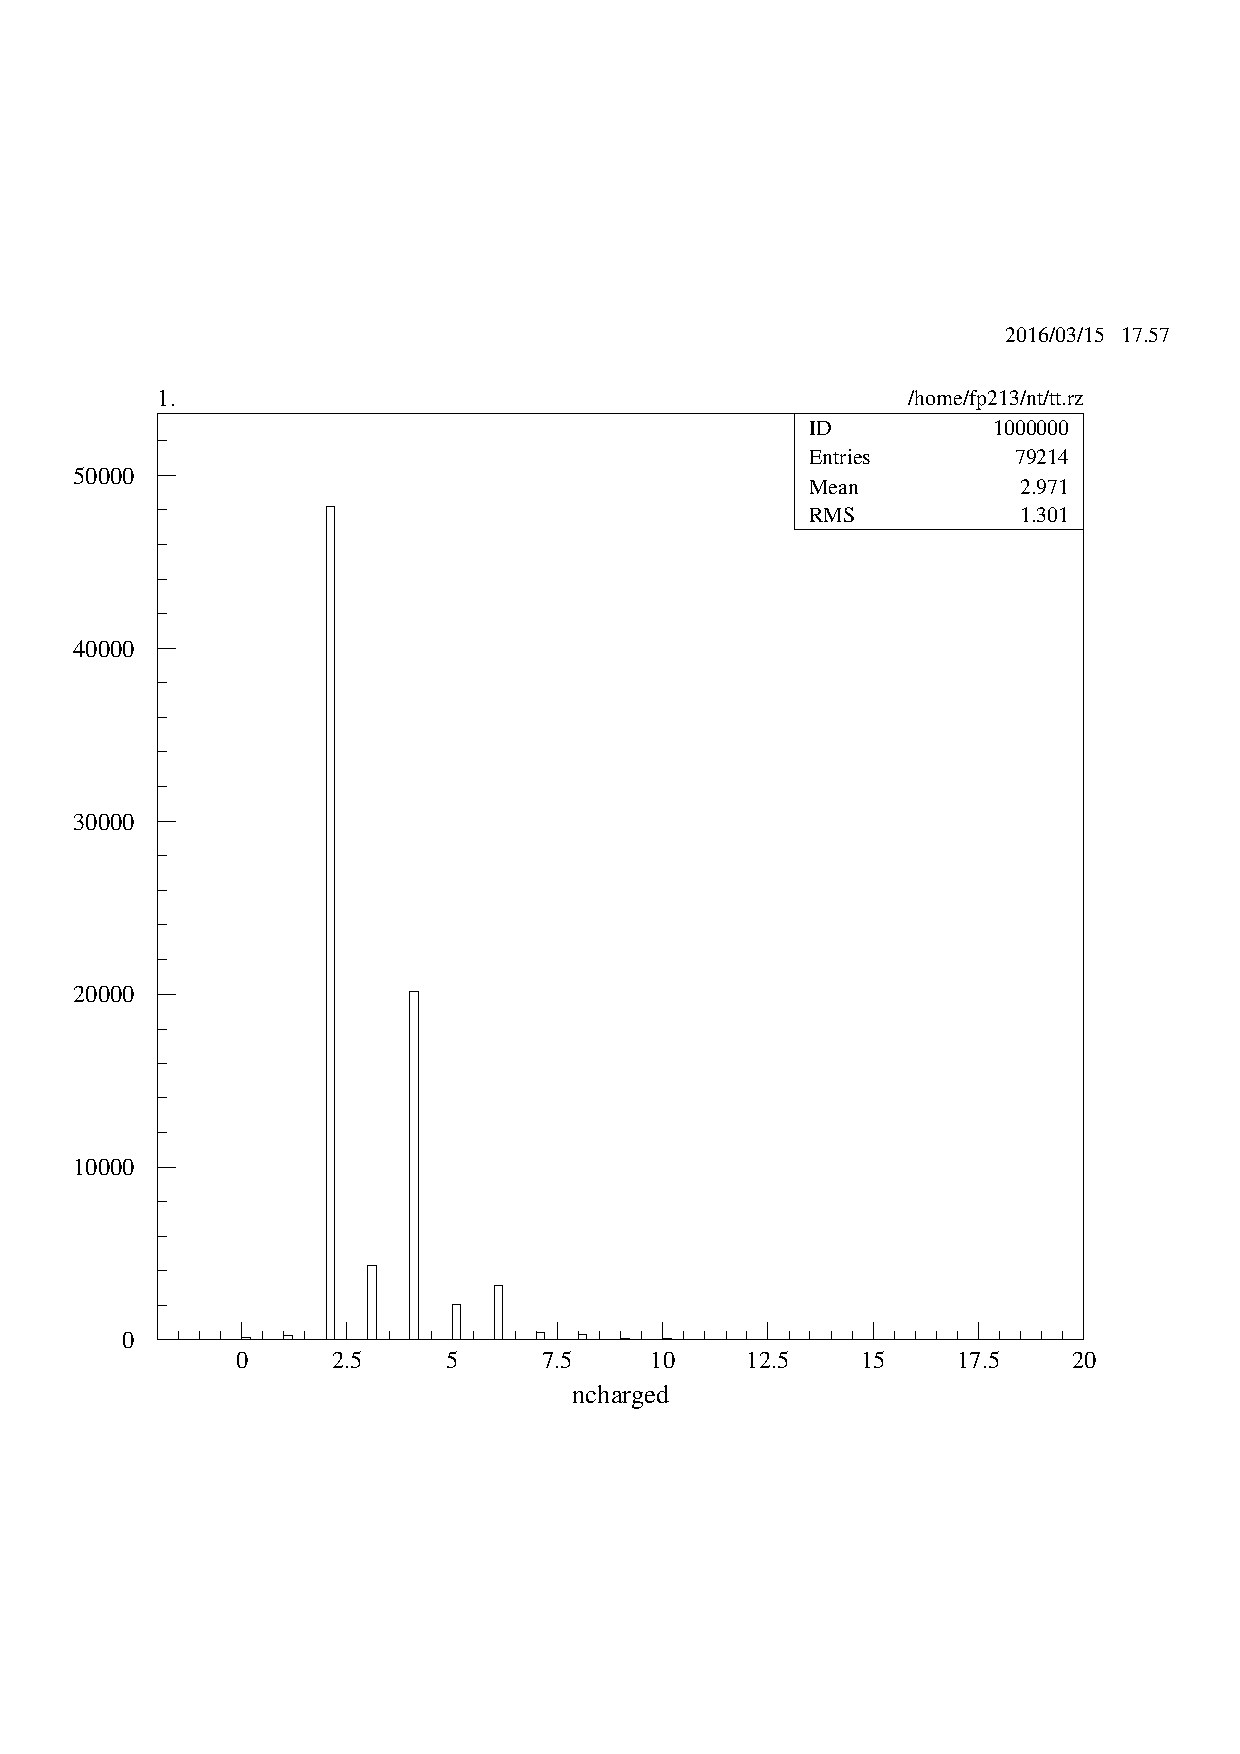
\includegraphics[width=\linewidth]{taus-ncharged}
        \caption{%
            Tauons
        }
        \label{fig:paw-ncharged/tuaons}
    \end{subfigure}
    \hfill
    \begin{subfigure}[c]{0.48\linewidth}
        \centering
        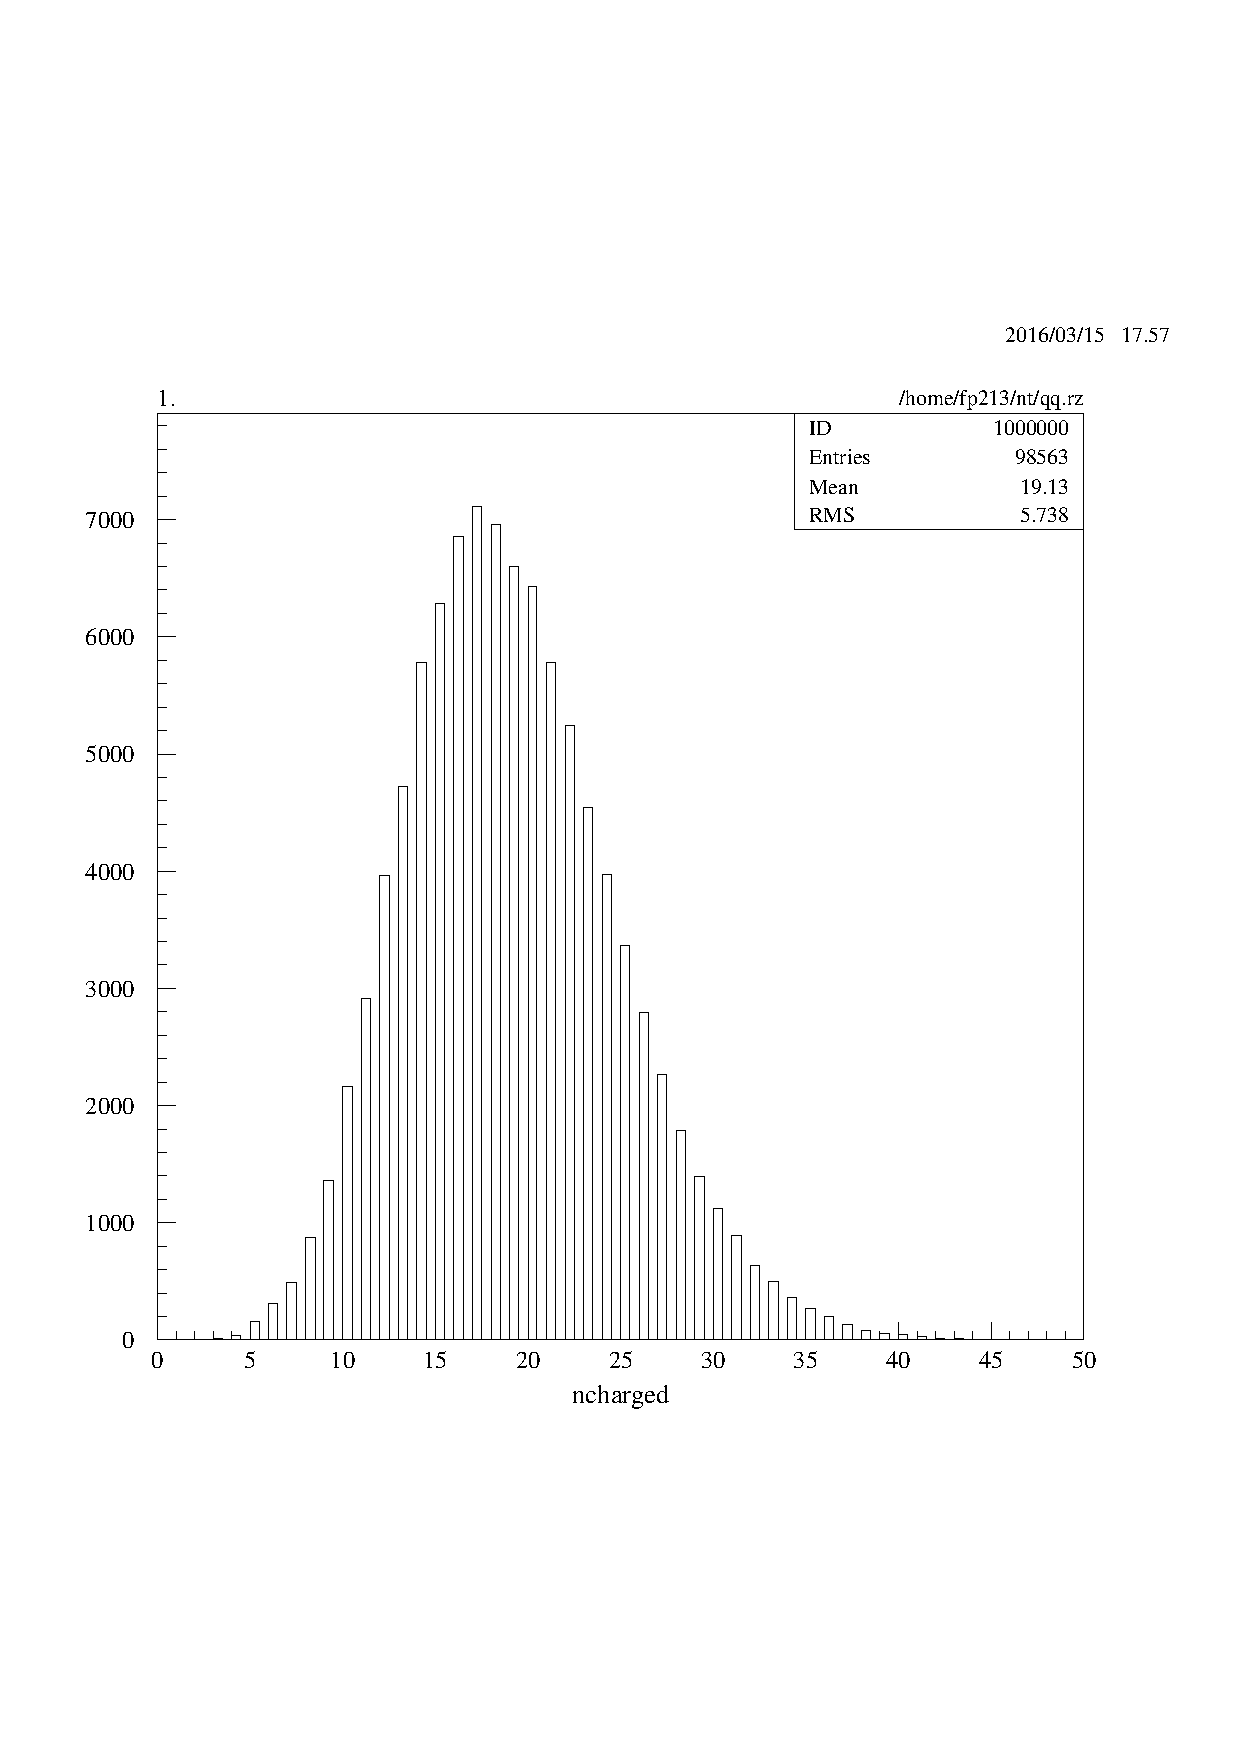
\includegraphics[width=\linewidth]{hadrons-ncharged}
        \caption{%
            Hadrons
        }
        \label{fig:paw-ncharged/hadrons}
    \end{subfigure}

    \caption{%
        Number of charged tracks, \ncharged, for the four decay types.
        Histograms generated with \textsc{paw} from Monte Carlo datasets.
    }
    \label{fig:paw-ncharged}
\end{figure}


With a magnifying glass we can see that there are mostly two charged tracks for
electron and muon decays. Interestingly, there are occasionally three to four
tracks for the electron.

As expected from decay modes with hadrons, we see that taus can have six
charged tracks. Hadrons can also decay with six or less charged tracks, but the
most part decays with more than then tracks.

The other characteristics, were also plotted using \textsc{paw}. \pcharged\ is
shown in Figure~\ref{fig:paw-pcharged}, \eecal\ in Figure~\ref{fig:paw-e_ecal}
and \ehcal\ in Figure~\ref{fig:paw-e_hcal}.

\subsection{Angular distribution}

As one can see in Figure~\ref{fig:paw-angle}, the angular distribution of the
four decay modes is not the shifted parabola as expected from the $s$-channel
theory. For the electrons, this arises from the mixing with the $t$-channel. We
do not want to include the $t$-channel reactions as this would make a
comparison to the other leptonic channels (only $s$-channel) impossible.

We have shown in Figure~\ref{fig:channels} how the $s$- and $t$-channel scale
with the angle. At small angle, the unwanted $t$-channel dominates. Therefore
we need to cut large $\cos(\theta)$ out of our analysis. The efficiency will do
down, but the quality of the remaining data will be better. We also cut the
peak at $\cos(\theta) < -0.9$ as we do not know its origin but know that it
cannot come from a simple $s$-channel process.


\begin{figure}
    \centering
    \begin{subfigure}[c]{0.48\linewidth}
        \centering
        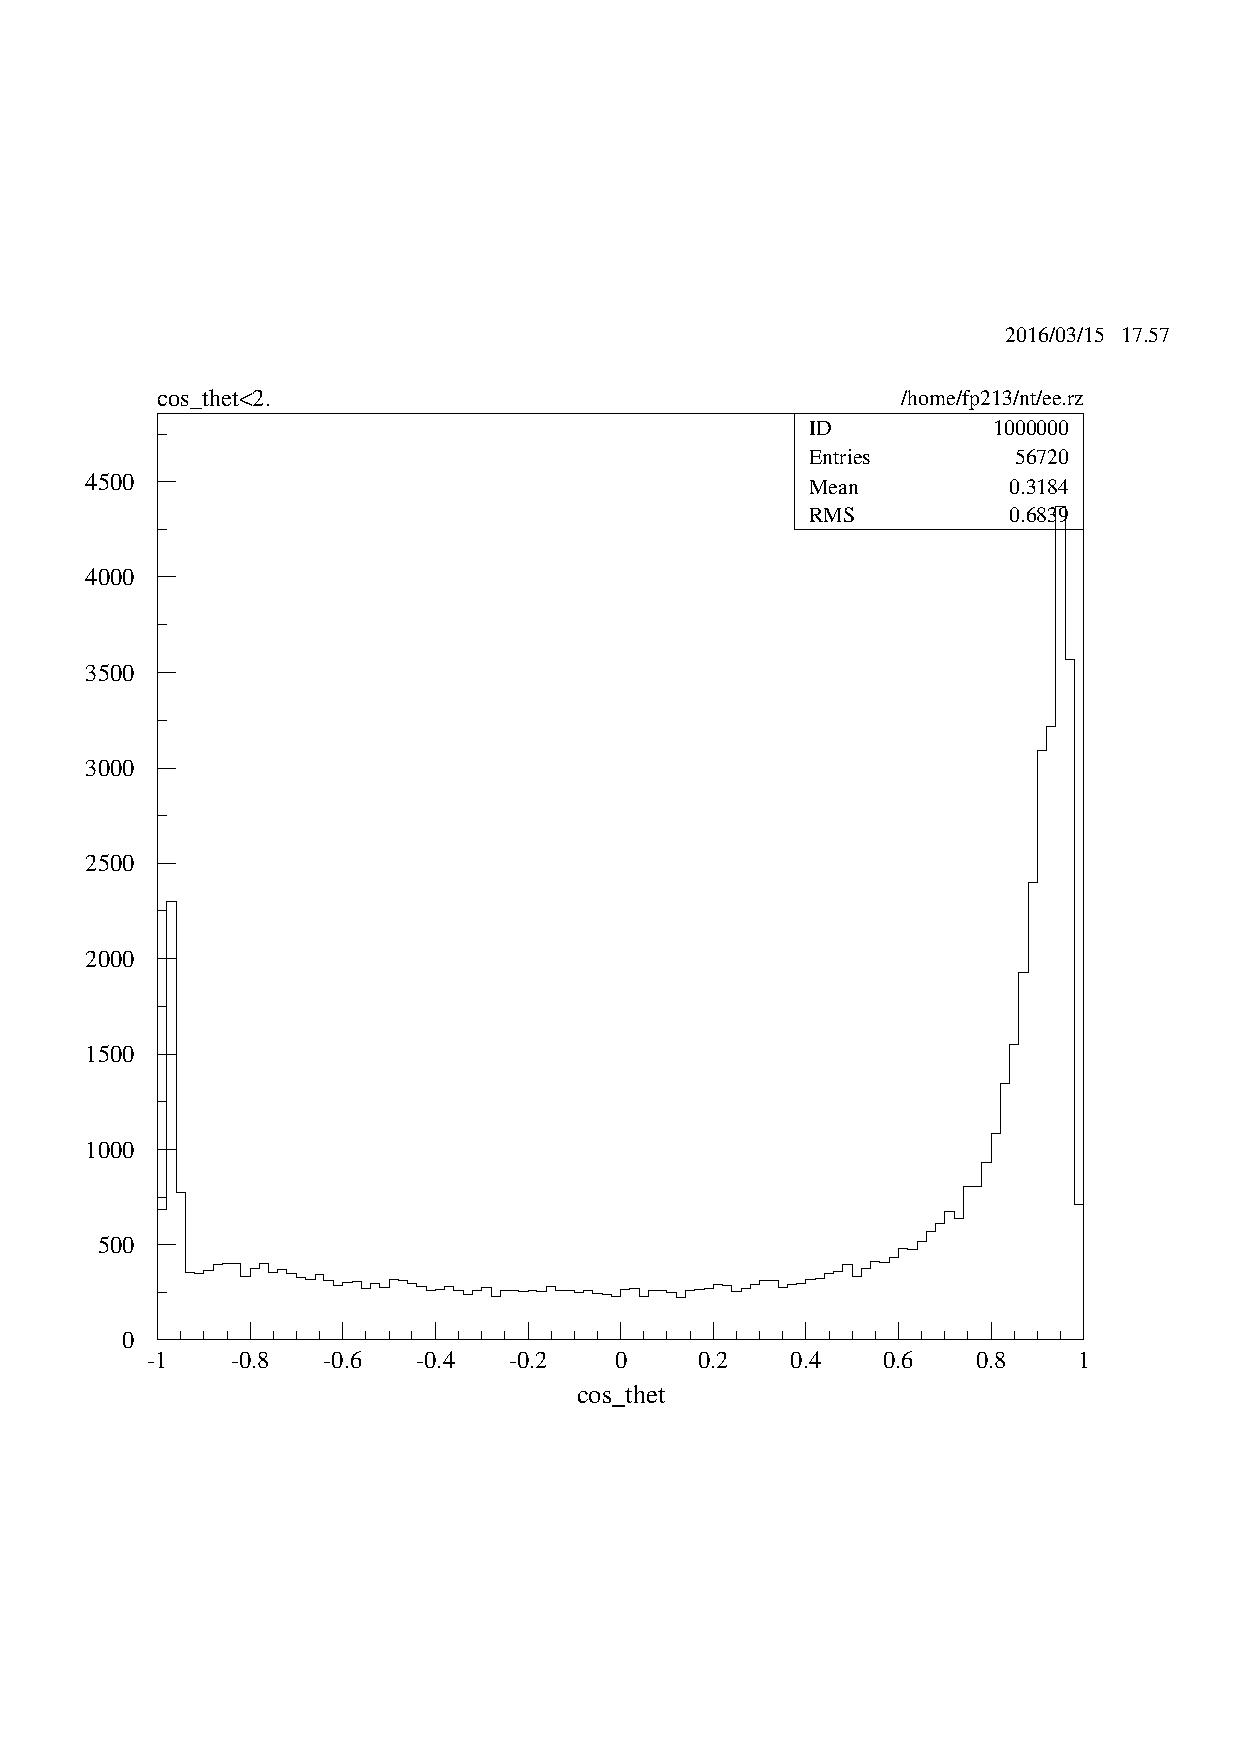
\includegraphics[width=\linewidth]{electrons-cos_thet}
        \caption{%
            Electrons
        }
        \label{fig:paw-angle/electrons}
    \end{subfigure}
    \hfill
    \begin{subfigure}[c]{0.48\linewidth}
        \centering
        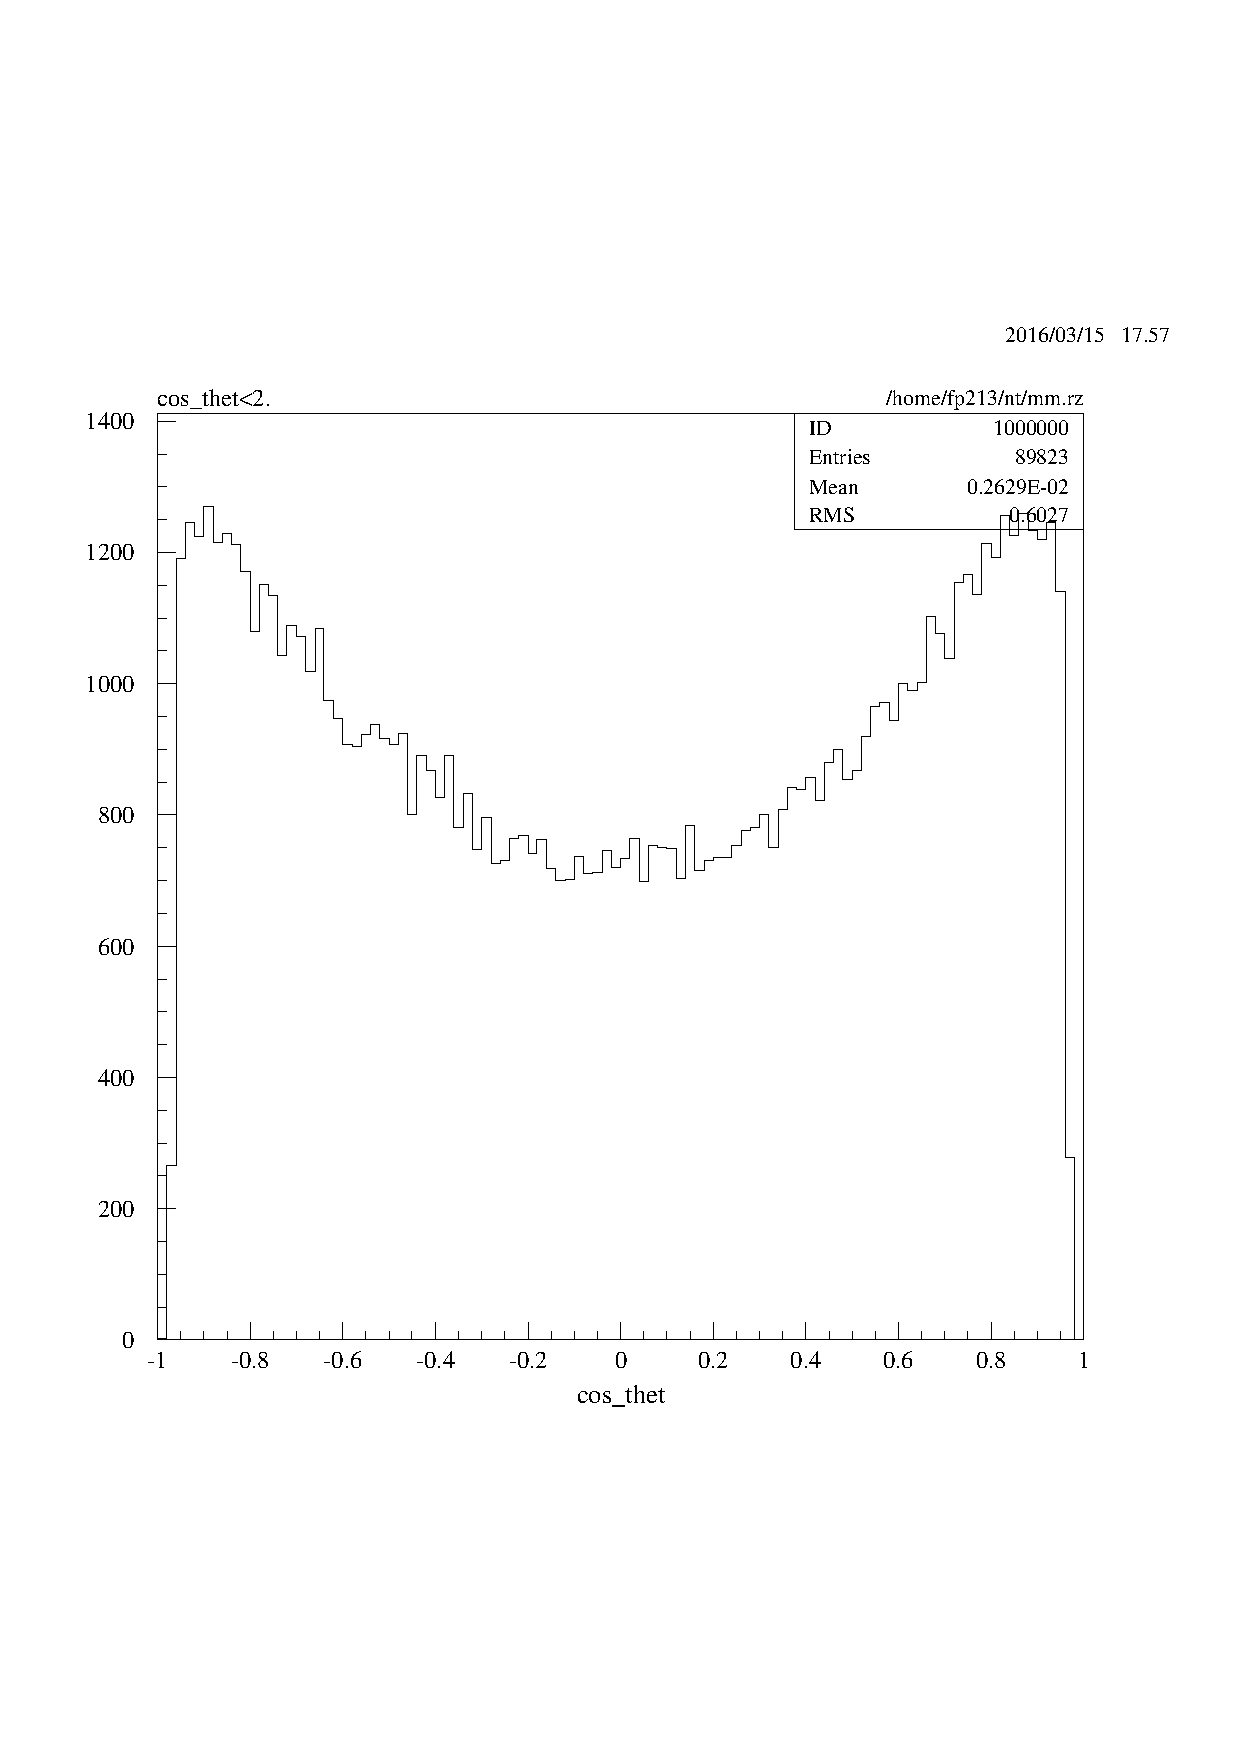
\includegraphics[width=\linewidth]{muons-cos_thet}
        \caption{%
            Muons
        }
        \label{fig:paw-angle/muons}
    \end{subfigure}

    \vspace{2ex}

    \begin{subfigure}[c]{0.48\linewidth}
        \centering
        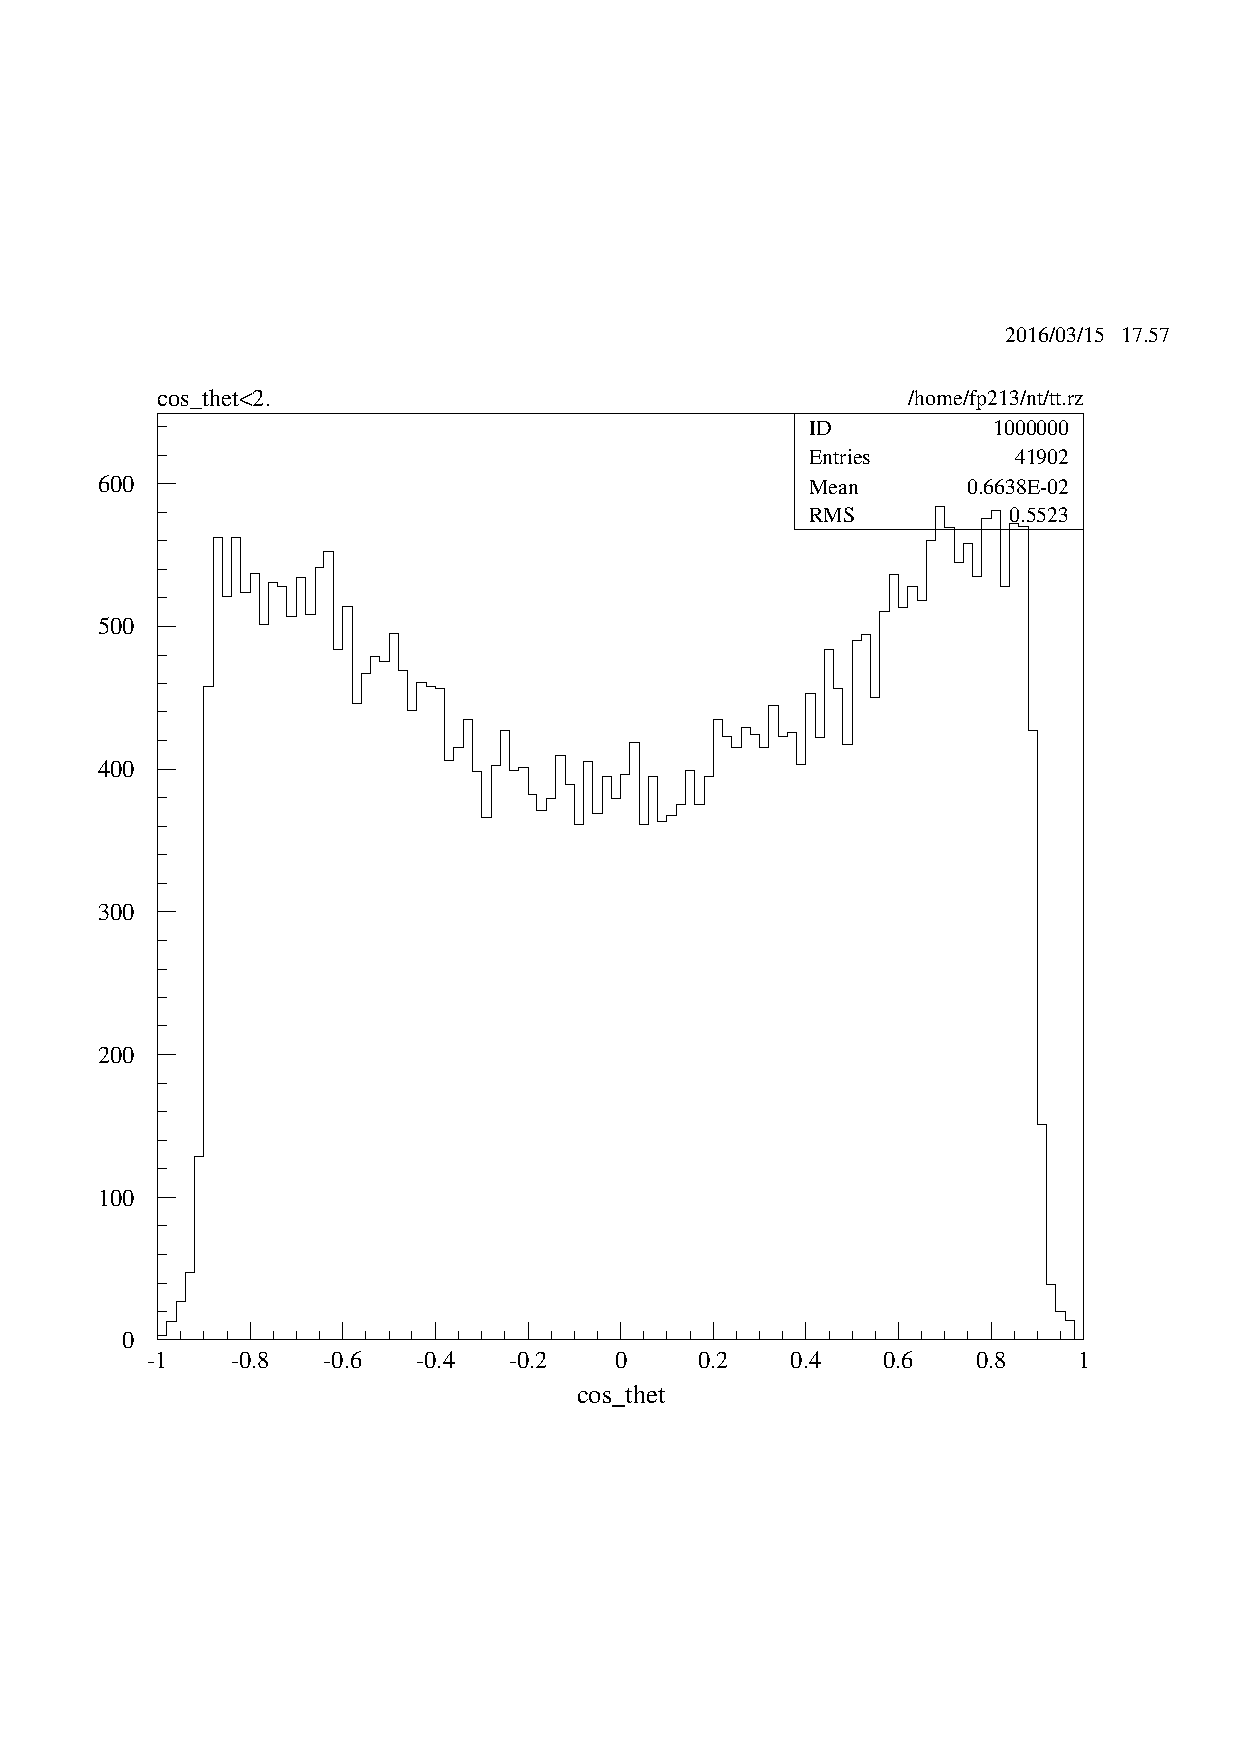
\includegraphics[width=\linewidth]{taus-cos_thet}
        \caption{%
            Tauons
        }
        \label{fig:paw-angle/tauons}
    \end{subfigure}
    \hfill
    \begin{subfigure}[c]{0.48\linewidth}
        \centering
        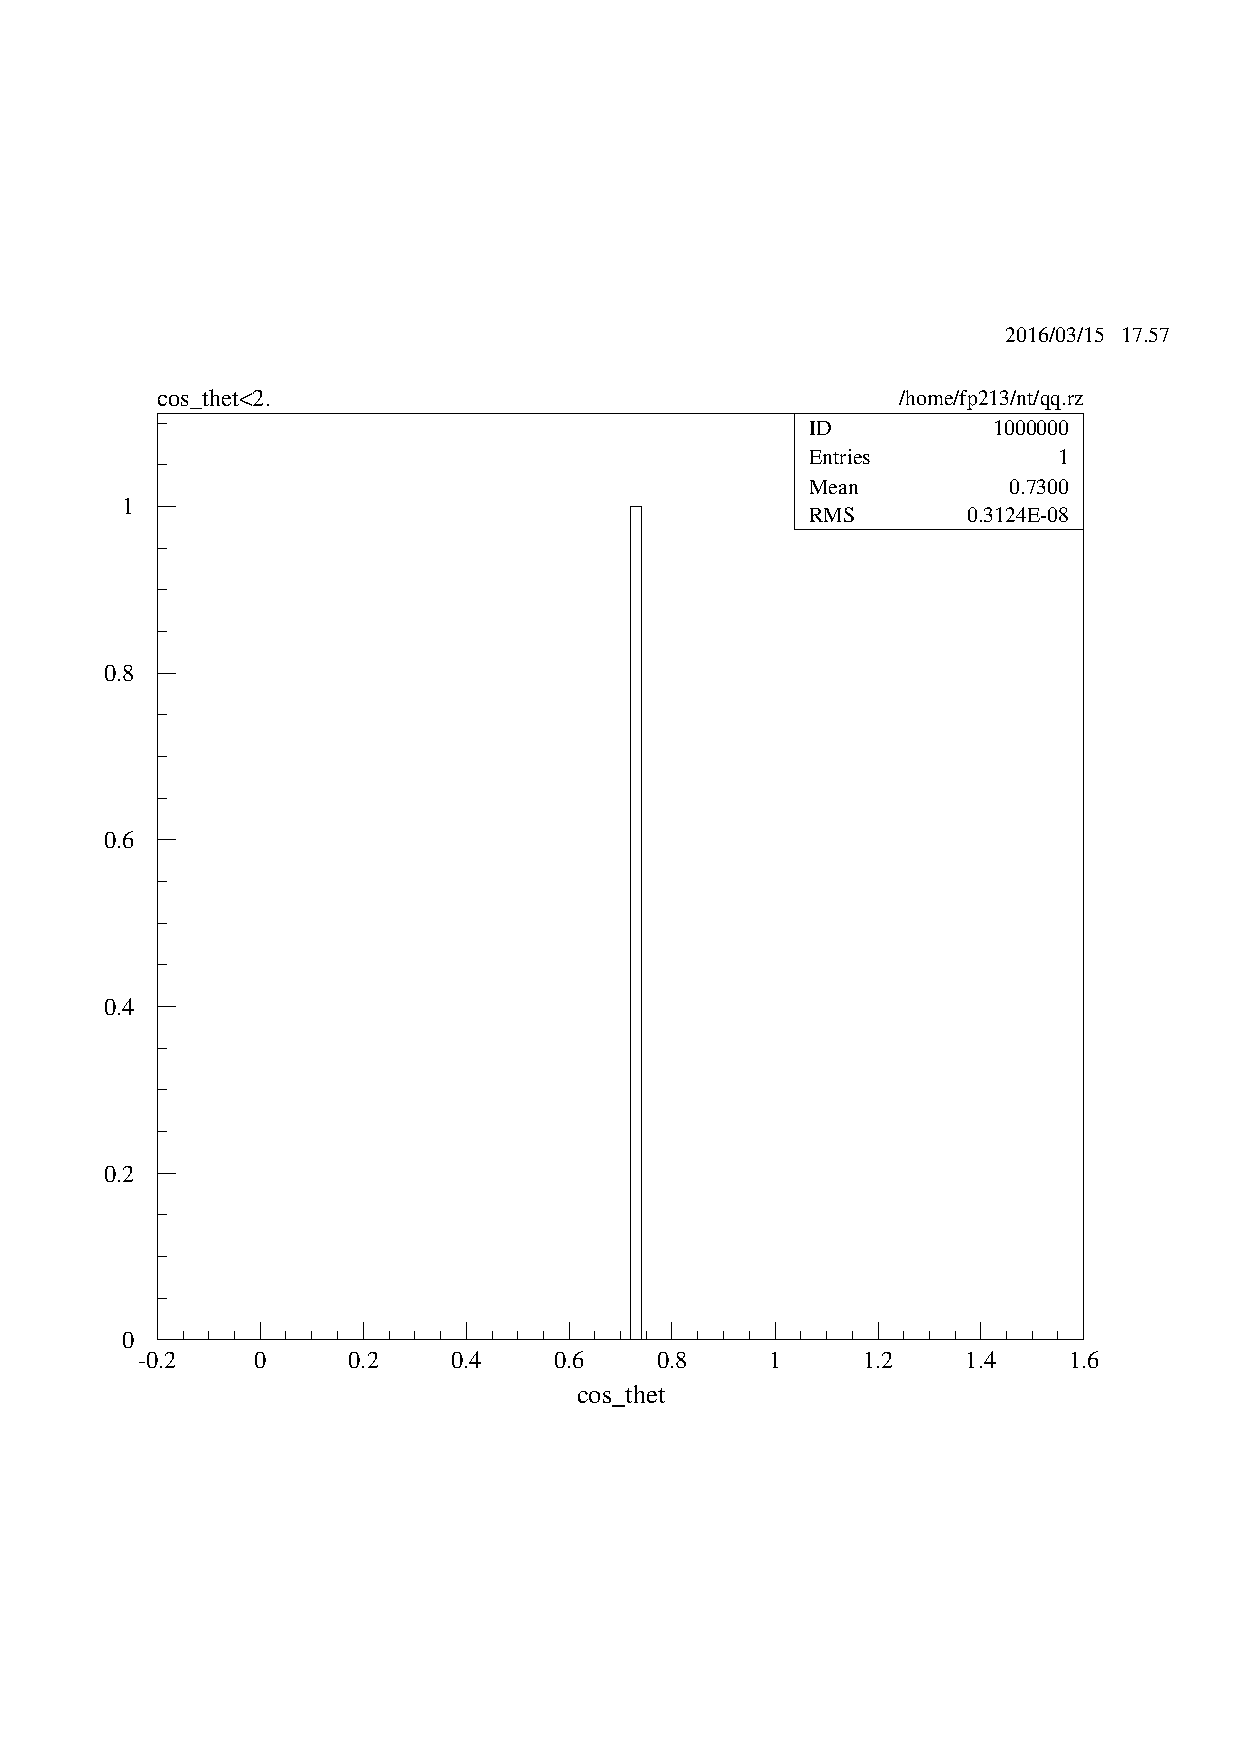
\includegraphics[width=\linewidth]{hadrons-cos_thet}
        \caption{%
            Hadrons
        }
        \label{fig:paw-angle/hadrons}
    \end{subfigure}

    \caption{%
        Angular distribution with respect to $\cos(\theta)$ for the four decay
        types. Histograms generated with \textsc{paw} from Monte Carlo
        datasets. Events without a defined angle are excluded, therefore there
        are no events with more or less than one positively charged track
        included.
    }
    \label{fig:paw-angle}
\end{figure}


The muons (see Figure~\ref{fig:paw-angle/muons}) look pretty good. At
$|\cos(\theta)| > 0.9$ we have a sharp drop which we blame on the detector not
covering the whole solid angle. Since the beam pipe needs to go through the
detector, one cannot detect collinear events. We therefore cut those events
away.

The shape of the taus (see Figure~\ref{fig:paw-angle/taus}) seems to be a
parabola in the middle but flatten off to the sides. Events with only one
charged positive track have to be a decay into an positron or an anti-muon. A
neutrino is created in those processes, skewing the angular distribution.
Therefore this flattening does not need to be cut out.

For the hadrons (see Figure~\ref{fig:paw-angle/hadrons}), an angular
distribution is rarely defined, there is only one event that even has a
well-defined $\theta$-angle. Therefore we do not perform any cutting in the
hadronic sector.

Our refined and final cuts including the angle are listed in
Table~\ref{tab:cuts2}.

\begin{table}
    \centering
    \begin{tabular}{lccccc}
        \toprule
        & \multicolumn{5}{c}{Cut criterion} \\
        \cmidrule(l){2-6}
        Particle
        & \ncharged
        & \sump/\si{\giga\electronvolt}
        & \eecal/\si{\giga\electronvolt}
        & \ehcal/\si{\giga\electronvolt}
        & $\cos(\theta)$
        \\
        \midrule
        Electrons & $< 4$ &  & $> 60$ &  & $\num{-.9}\leq\dots\leq\num{.5}$ \\
        Muons & $< 4$ & $> 75$ & $< 20$ &  & $\num{-.9}\leq\dots\leq\num{.9}$ \\
        Taus & $< 7$ & $< 75$ & $\leq 75$ &  &\\
        Hadrons & $> 7$ &  &  &  & \\
        \bottomrule
    \end{tabular}
    \caption{%
        Cuts derived from the full Monte Carlo datasets.
    }
    \label{tab:cuts2}
\end{table}

\section{Muon forward--backward asymmetry}

The muon forward--backward asymmetry is a quantity that we want to extract from
the data. For this we need to filter the actual dataset (in our case number 1)
for muons. Then we also need to filter by beam energy. The dataset contains
seven different beam energies, we define seven more filters like the following:

\begin{lstlisting}
nt/cuts $11 e_lep>44.0.and.e_lep<44.5
nt/cuts $12 e_lep>44.5.and.e_lep<45.0
\end{lstlisting}

Using those, we can filter the data for muons (\texttt{\$2}), positive or
negative angle (\texttt{cos\_thet<0.} or \texttt{cos\_thet>0}) and for the energy (\texttt{\$11}). Printing this as
a histogram, we use the following code:

\begin{lstlisting}
nt/plot daten1.cos_thet $2.and.cos_thet<0..and.$11
pict/print afb-muons-daten1-negative-energy1.ps
nt/plot daten1.cos_thet $2.and.cos_thet>0..and.cos_thet<2..and.$11
pict/print afb-muons-daten1-positive-energy1.ps
\end{lstlisting}

We have also supplied the additional criterion for sensible angles
(\texttt{cos\_thet<2.}) because undefined angles have a numerical value way
greater than two.

From the exported diagrams (not included in this report) we extract the number
of events with $\cos(\theta) > 0$, which we call $N_+$, and the events with
$\cos(\theta) < 0$, which we call $N_-$. The asymmetry is then simply
\[
    A_\text{FB} = \frac{N_+ - N_-}{N_+ + N_-} \,.
\]

Our analysis to this point is based on the tree level formalism. Higher order
corrections are needed in every QFT for more accurate result. Here we are given
the combined effect of all those corrections as a table of shift for
$A_\text{FB}$. For each beam energy, we add the correction and obtain a final
value for $A_\text{FB}$. The resulting asymmetry for the different beam
energies is shown in Figure~\ref{fig:plot-afb}. Error estimation is done by
assuming an error of $\sqrt{N}$ for all the counts and using Gaussian error
propagation for the final result.

\begin{figure}
    \centering
    \includegraphics{plot-afb}
    \caption{%
        Forward--backward asymmetry in the muon events. Shown are both
        uncorrected and corrected values for $A_\text{FB}$. Both values have
        the same error, therefore we only show the error bar for the corrected
        values.
    }
    \label{fig:plot-afb}
\end{figure}

The figure also includes the theoretical expectation that we have computed in
the exercises in Section~\ref{sec:exercises-asymmetry}. We have re-computed the
expectation value with the physical value of $\sin(\theta_\text w)^2$ for the
various beam energies used. Our results do not imply this exact trend (i.e.\
almost constant) of the asymmetry. However, as the errors are quite large, our
measurements are still consistent with it.

\section{Detection efficiency}
\label{sec:detection-efficiency}

By choosing the cuts in a particular way, we make a compromise between
detection efficiency and underground. Choosing a tight cut will discard events
that should have been counted. This will lead to a loss of a certain fractions
of events. This is not directly a problem as we can just compensate by this
loss factor. However, our statistical errors will grow as we have less
statistics. A loose cut will water the sorting with underground events. Say we
want to filter out electrons but our cuts are too loose. Then some tau events
might slip into the electrons category.

Both types of errors, the false-negatives and the false-positives, can be
handled using a detection matrix~$\mat D$ and Monte Carlo datasets.
The Monte Carlo datasets are purely of one decay channel. Therefore we know
exactly that we only have, say, electrons. Applying our cuts to the Monte Carlo
electrons, we will see how many are actually detected as electrons. This is our
efficiency. Then we take the other three kinds (muons, taus, hadrons) of the
Monte Carlo datasets and apply the electron cuts to it. Ideally, we should not
get any events. The ratio of other events that we falsely identify as electrons
is the underground.

Using a linear model for this, we need a mapping from the actual events vector
$\vec A$ (in electron-muon-tau-hadrons space, $\N^4$) to the identified events
vector $\vec I$ (same space). The detection matrix is then defined via $\vec I
= \mat D \vec A$. In order to find the sixteen matrix elements, we apply a
vector with Monte Carlo electrons.

% TODO Explain efficiency of electrons is wrong due to cut in angle, we
% introduce the t-channel back with the method that we have used here.

\subsection{Determining matrix elements}

In order to do this with \textsc{paw}, we define our final cuts for electrons,
muons, taus and hadrons:

\begin{lstlisting}
nt/cuts $1 ncharged<4.and.e_ecal>60.and.cos_thet<.5.and.cos_thet>-0.9
nt/cuts $2 pcharged>75.and.ncharged<4.and.e_ecal<20.and.cos_thet<.9.and.cos_thet>-0.9
nt/cuts $3 pcharged<75.and.ncharged<7.and.e_ecal<75
nt/cuts $4 ncharged>7
\end{lstlisting}

We need to count the number of events that matched a given cut. Creating a
histogram with respect to an arbitrary characteristic will give us this number
as a side effect. The following generates a histogram with electron data and
the electron filter:

\begin{lstlisting}
nt/plot electrons.ncharged $1
pict/print matrix-electrons-with-electron-filter.ps
\end{lstlisting}

And this generates a histogram with muon data and the same filter:

\begin{lstlisting}
nt/plot muons.ncharged $1
pict/print matrix-muons-with-electron-filter.ps
\end{lstlisting}

Similar expressions are needed for the other matrix element, in total we need
16 of those counting histograms. The resulting histograms are shown in
Figure~\ref{fig:paw-matrix-electrons}. Squint at the row \enquote{Entries} in
the legend, this is the interesting number.

For the electrons, the input vector is $\vec A = (94381, 0, 0,
0)^\mathrm T$. Then we look at the output and find $\vec I = (20474, 1, 1013,
0)^\mathrm T$. From this, we can construct the first row in the matrix. Using
the other filters, we can construct the whole matrix. Figure~\ref{fig:matrix/1}
shows the matrix. It can be seen that it is mostly diagonal, just as we want it
to be. The detection efficiency for the electrons is not very great. This comes
from the severe cutting in $\cos(\theta) < 0.5$ which discards a lot of events.

%\begin{figure}
%    \centering
%    \begin{subfigure}[t]{0.48\linewidth}
%        \centering
%        %\includegraphics[width=\linewidth]{mpl-normalized_matrix}
%        \caption{%
%            Detection matrix. Left-multiply with a vector which contains actual
%            event numbers to get event numbers identified by our cuts.
%        }
%        \label{fig:matrix/1}
%    \end{subfigure}
%    \hfill
%    \begin{subfigure}[t]{0.48\linewidth}
%        \centering
%        %\includegraphics[width=\linewidth]{mpl-inverted_matrix}
%        \caption{%
%            Inverse matrix. Left-multiply with a vector containing our
%            measurements to get actual event numbers.
%        }
%        \label{fig:matrix/2}
%    \end{subfigure}
%    \caption{%
%        Normalized conversion matrices between detected and actual event types.
%    }
%    \label{fig:matrix}
%\end{figure}

\begin{table}
    \centering
    \begin{tabular}{lSSSS}
        \toprule
        & \multicolumn{4}{c}{Acceptance rate / \si{\percent}} \\
        \cmidrule(l){2-5}
        {Detected as}
        & {Electrons}
        & {Muons}
        & {Taus}
        & {Hadrons} \\
        \midrule
        %< for row in matrix >%
        << ' & '.join(row) >> \\
        %< endfor >%
        \bottomrule
    \end{tabular}
    \caption{%
        The detection matrix $\mat D$. Although it is displayed in a table, it is meant
        as a matrix which can be right-multiplied with an actual events
        vector $\vec A$. The resulting vector will be the vector of identified
        events $\vec I$ of our cuts. The matrix is mostly diagonal, the low
        number for electron--electron is due to our mistake in angular
        restriction (see text).
    }
    \label{tab:matrix}
\end{table}

\begin{table}
    \centering
    \begin{tabular}{lllll}
        \toprule
        & \multicolumn{4}{c}{Correction factor} \\
        \cmidrule(l){2-5}
        {Actually are}
        & {Electrons}
        & {Muons}
        & {Taus}
        & {Hadrons} \\
        \midrule
        %< for row in inverted >%
        << ' & '.join(row) >> \\
        %< endfor >%
        \bottomrule
    \end{tabular}
    \caption{%
        The inverted detection matrix $\mat D\inv$.
    }
    \label{tab:inverted}
\end{table}



\subsection{Inverting the matrix}

In order to use this detection matrix~$\mat E$ as a correction, we need to
invert the matrix. As it is almost diagonal, this will be numerically stable.
The inverted matrix is visualized in Figure~\ref{fig:matrix/2}.

% TODO Error calculation.

\section{Partial cross sections}

\subsection{Counts}

In order to compute cross sections, we need count rates. We have filtered the
dataset with our cuts and an energy selection. For instance the following
snippet we use the muon filter (\texttt{\$2}) with the third beam energy
(\texttt{\$13}):

\begin{lstlisting}
nt/plot daten1.ncharged $2.and.$13
pict/print filtered-daten1-as-muon-energy3.ps
\end{lstlisting}

The full code listing can be found in Section~\ref{data-cuts.kumac}. We look at
the generated histograms and extract the number of events from each histogram.
The results are collected in Table~\ref{tab:counts}. Not shown is the error
which we assume to be $\sqrt{N}$ as this is a counting experiment.

\begin{table}
    \centering
    \begin{tabular}{SSSSS}
        \toprule
        & \multicolumn{4}{c}{Raw count} \\
        \cmidrule(l){2-5}
        {$\sqrt s / \si{\giga\electronvolt}$}
        & {Electrons}
        & {Muons}
        & {Taus}
        & {Hadrons} \\
        \midrule
        %< for row in counts_table >%
        << ' & '.join(row) >> \\
        %< endfor >%
        \bottomrule
    \end{tabular}
    \caption{%
        Raw counts for the four decay types and seven beam energies.
    }
    \label{tab:counts}
\end{table}

Those counts are just the counts which are left after applying the cuts. As
argued in regarding the detection efficiency (c.f.\
Section~\ref{sec:detection-efficiency}), those counts include some number of
false-positives (underground) and false-negatives (inefficiency). Therefore we
need to correct for that with the inverse matrix derived above.

Taking the four counts at each beam energy as a \enquote{identified events}
vector $\vec I$, we can use $\mat D\inv$ to give us the \enquote{actual events}
vector $\vec A$. We do this for each of the seven beam energies and obtain the
corrected counts. Those are shown in Table~\ref{tab:corrected-counts}.

\begin{table}
    \centering
    \begin{tabular}{SSSSS}
        \toprule
        & \multicolumn{4}{c}{Corrected count} \\
        \cmidrule(l){2-5}
        {$\sqrt s / \si{\giga\electronvolt}$}
        & {Electrons}
        & {Muons}
        & {Taus}
        & {Hadrons} \\
        \midrule
        %< for row in corrected_counts_table ->%
        << ' & '.join(row) >> \\
        %< endfor ->%
        \bottomrule
    \end{tabular}
    \caption{%
        Corrected counts for the four decay types and seven beam energies.
    }
    \label{tab:corrected-counts}
\end{table}

\subsection{Incorporating the luminosity}

We want to compute the partial cross sections, those are the cross sections of
the individual decay channels. For this we just need to take the number of
counts in each channel and divide by the integrated luminosity. Therefore we
have
\[
    \sigma_i = \frac{N_i}{\int \dif t \, \mathcal L} \,.
\]

Table~\ref{tab:luminosities} lists the integrated luminosities for our dataset.

\begin{table}
    \centering
    \begin{tabular}{SS}
        \toprule
        {$\sqrt s / \si{\giga\electronvolt}$}
        & {$\int \dif t \, \mathcal L / \si{\per\nano\barn}$} \\
        \midrule
        %< for row in luminosities_table >%
        << ' & '.join(row) >> \\
        %< endfor >%
        \bottomrule
    \end{tabular}
    \caption{%
        Integrated luminosities $\int \dif t \, \mathcal L$ for the seven beam
        energies. The values are taken from the experiment description, the
        error is the total error (combined statistical and systematic error).
    }
    \label{tab:luminosities}
\end{table}

\begin{table}
    \centering
    \begin{tabular}{SSSSS}
        \toprule
        & \multicolumn{4}{c}{$\sigma_i / \si{\nano\barn}$} \\
        \cmidrule(l){2-5}
        {$\sqrt s / \si{\giga\electronvolt}$}
        & {Electrons}
        & {Muons}
        & {Taus}
        & {Hadrons} \\
        \midrule
        %< for row in cross_sections_table >%
        << ' & '.join(row) >> \\
        %< endfor >%
        \bottomrule
    \end{tabular}
    \caption{%
        Cross sections for the four decay types and seven beam energies.
    }
    \label{tab:cross-sections}
\end{table}

\begin{figure}
    \centering
    \includegraphics{cross-sections}
    \caption{%
        Partial cross sections for each type of final state. One can see that
        the leptonic cross sections are all similar, as expected. The hadronic
        cross section has to be $N_\text f N_\text c = 5 \cdot 3 = 15$ larger
        than the one in the single leptonic channels.
    }
    \label{fig:cross-sections}
\end{figure}

\definecolor{four1}{rgb}{0.21568627450980393,0.49411764705882355,0.7215686274509804}
\definecolor{four2}{rgb}{0.596078431372549,0.3058823529411765,0.6392156862745098}
\definecolor{four3}{rgb}{0.30196078431372547,0.6862745098039216,0.2901960784313726}
\definecolor{four4}{rgb}{0.8941176470588236,0.10196078431372549,0.10980392156862745}


\begin{tikzpicture}
    \begin{axis}[
            width=\linewidth,
            height=0.6\linewidth,
            xlabel={CMS Energy $\sqrt{s} / \si{\giga\electronvolt}$},
            ylabel={$\sigma_i / \si{\nano\barn}$},
            grid=major,
            legend pos=north west,
            mymarker/.style={
                mark=+,
                only marks,
                error bars/y dir=both,
                error bars/y explicit,
            },
            band/.style={
                draw=none,
                opacity=0.3,
            },
        ]

        \addplot[
            electrons,
            mymarker,
        ] table[y error index=2] {../xy/cross_section-electrons.tsv};
        \addlegendentry{Electrons}

        \addplot[
            muons,
            mymarker,
        ] table[y error index=2] {../xy/cross_section-muons.tsv};
        \addlegendentry{Muons}

        \addplot[
            taus,
            mymarker,
        ] table[y error index=2] {../xy/cross_section-taus.tsv};
        \addlegendentry{Tauons}

        \addplot[
            hadrons,
            mymarker,
        ] table[y error index=2] {../xy/cross_section-hadrons.tsv};
        \addlegendentry{Hadrons}

        \addplot [band, fill=electrons] table {../xy/cross_section-electrons-band.tsv} \closedcycle;
        \addplot [band, fill=muons] table {../xy/cross_section-muons-band.tsv} \closedcycle;
        \addplot [band, fill=taus] table {../xy/cross_section-taus-band.tsv} \closedcycle;
        \addplot [band, fill=hadrons] table {../xy/cross_section-hadrons-band.tsv} \closedcycle;


    \end{axis}
\end{tikzpicture}


\section{Decay widths}

\begin{table}
    \centering
    \begin{tabular}{lSS}
        \toprule
        Type
        & {$\MZ / \si{\giga\electronvolt}$}
        & {$\Gamma_i / \si{\giga\electronvolt}$} \\
        \midrule
        %< for row in lorentz_fits_table >%
        << ' & '.join(row) >> \\
        %< endfor >%
        \bottomrule
    \end{tabular}
    \caption{%
        Fit parameters of the Lorentzian curves used in
        Figure~\ref{fig:cross-sections} for the partial cross sections.
    }
    \label{tab:lorentz-fits}
\end{table}

%< if True >%
\begin{appendix}

    \chapter{PAW Histograms}

    \section{Monte Carlo data}

    \begin{figure}[h!]
    \centering
    \begin{subfigure}[c]{0.48\linewidth}
        \centering
        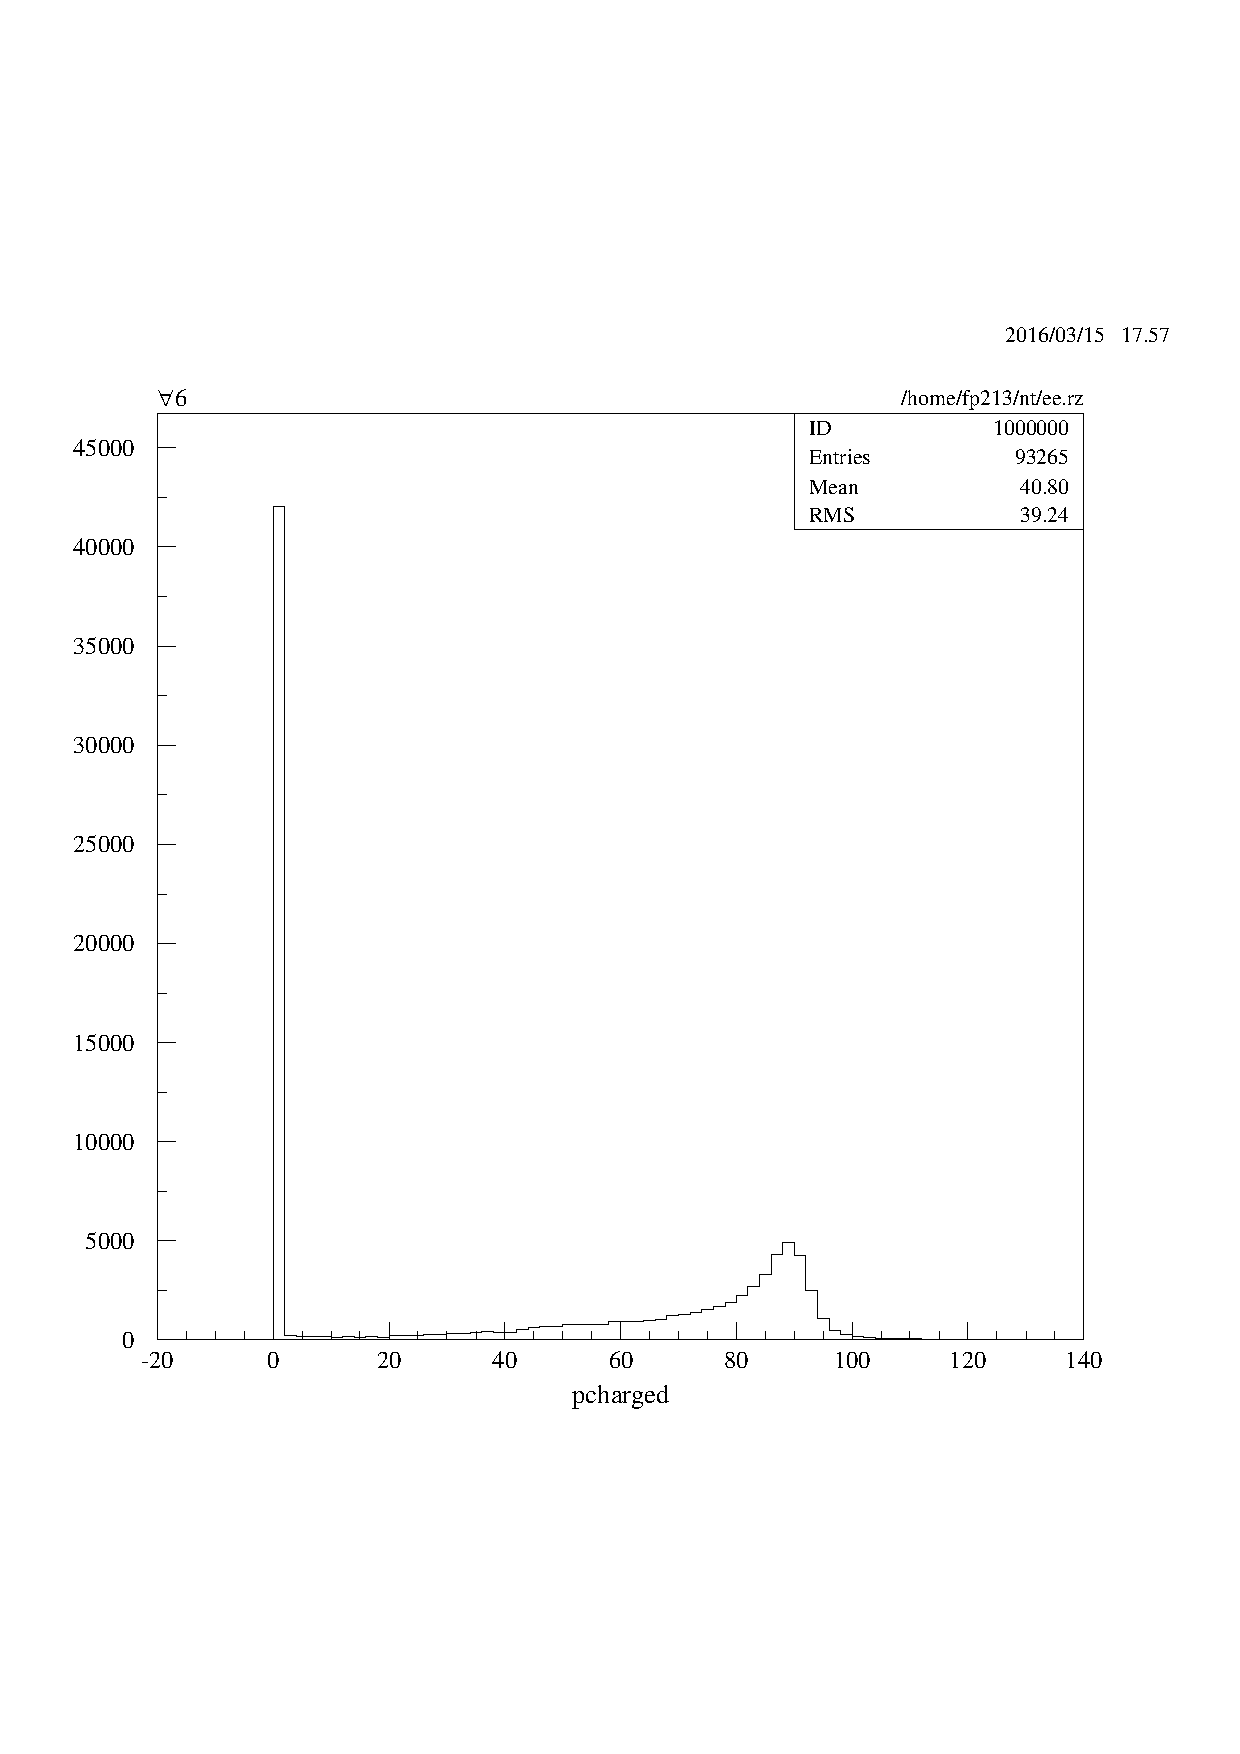
\includegraphics[width=\linewidth]{electrons-pcharged}
        \caption{%
            Electrons
        }
        \label{fig:paw-pcharged/electrons}
    \end{subfigure}
    \hfill
    \begin{subfigure}[c]{0.48\linewidth}
        \centering
        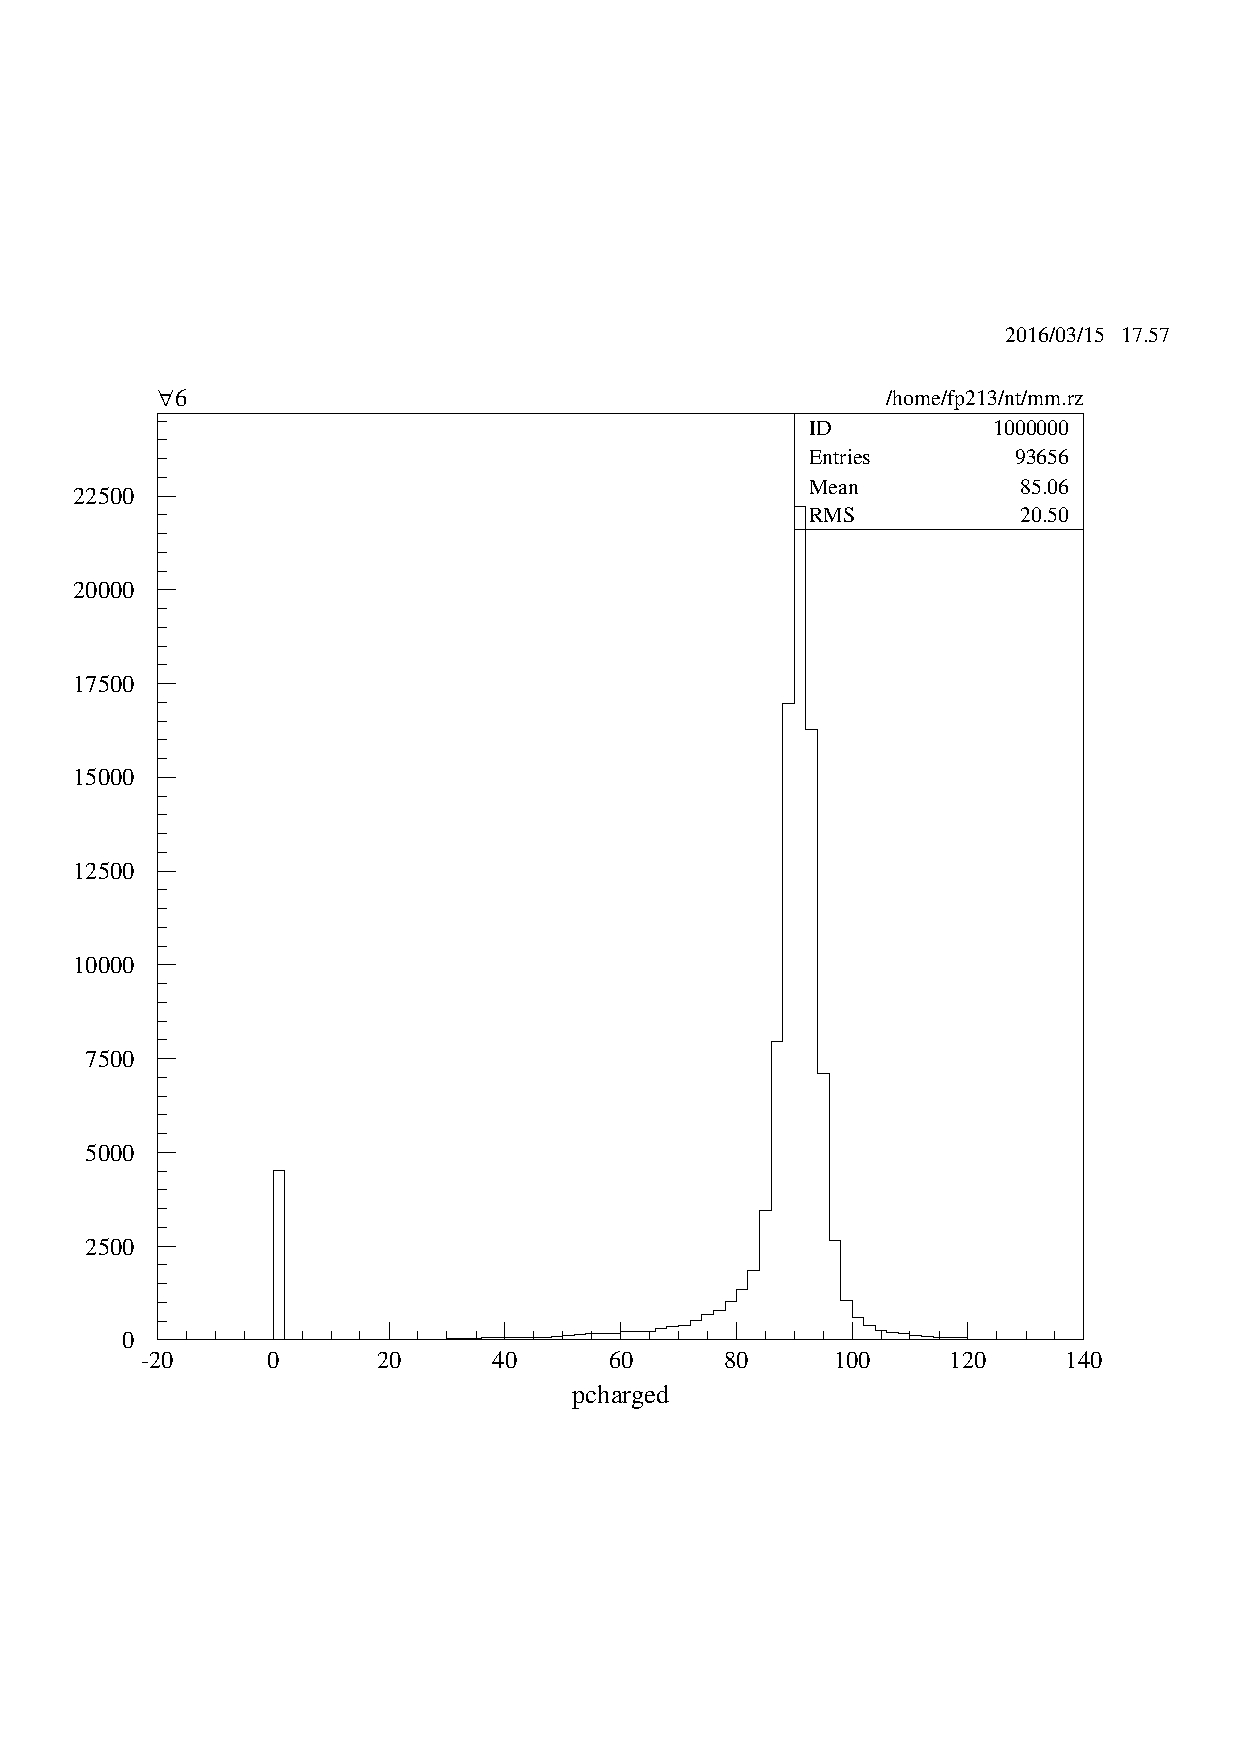
\includegraphics[width=\linewidth]{muons-pcharged}
        \caption{%
            Muons
        }
        \label{fig:paw-pcharged/muons}
    \end{subfigure}

    \vspace{2ex}

    \begin{subfigure}[c]{0.48\linewidth}
        \centering
        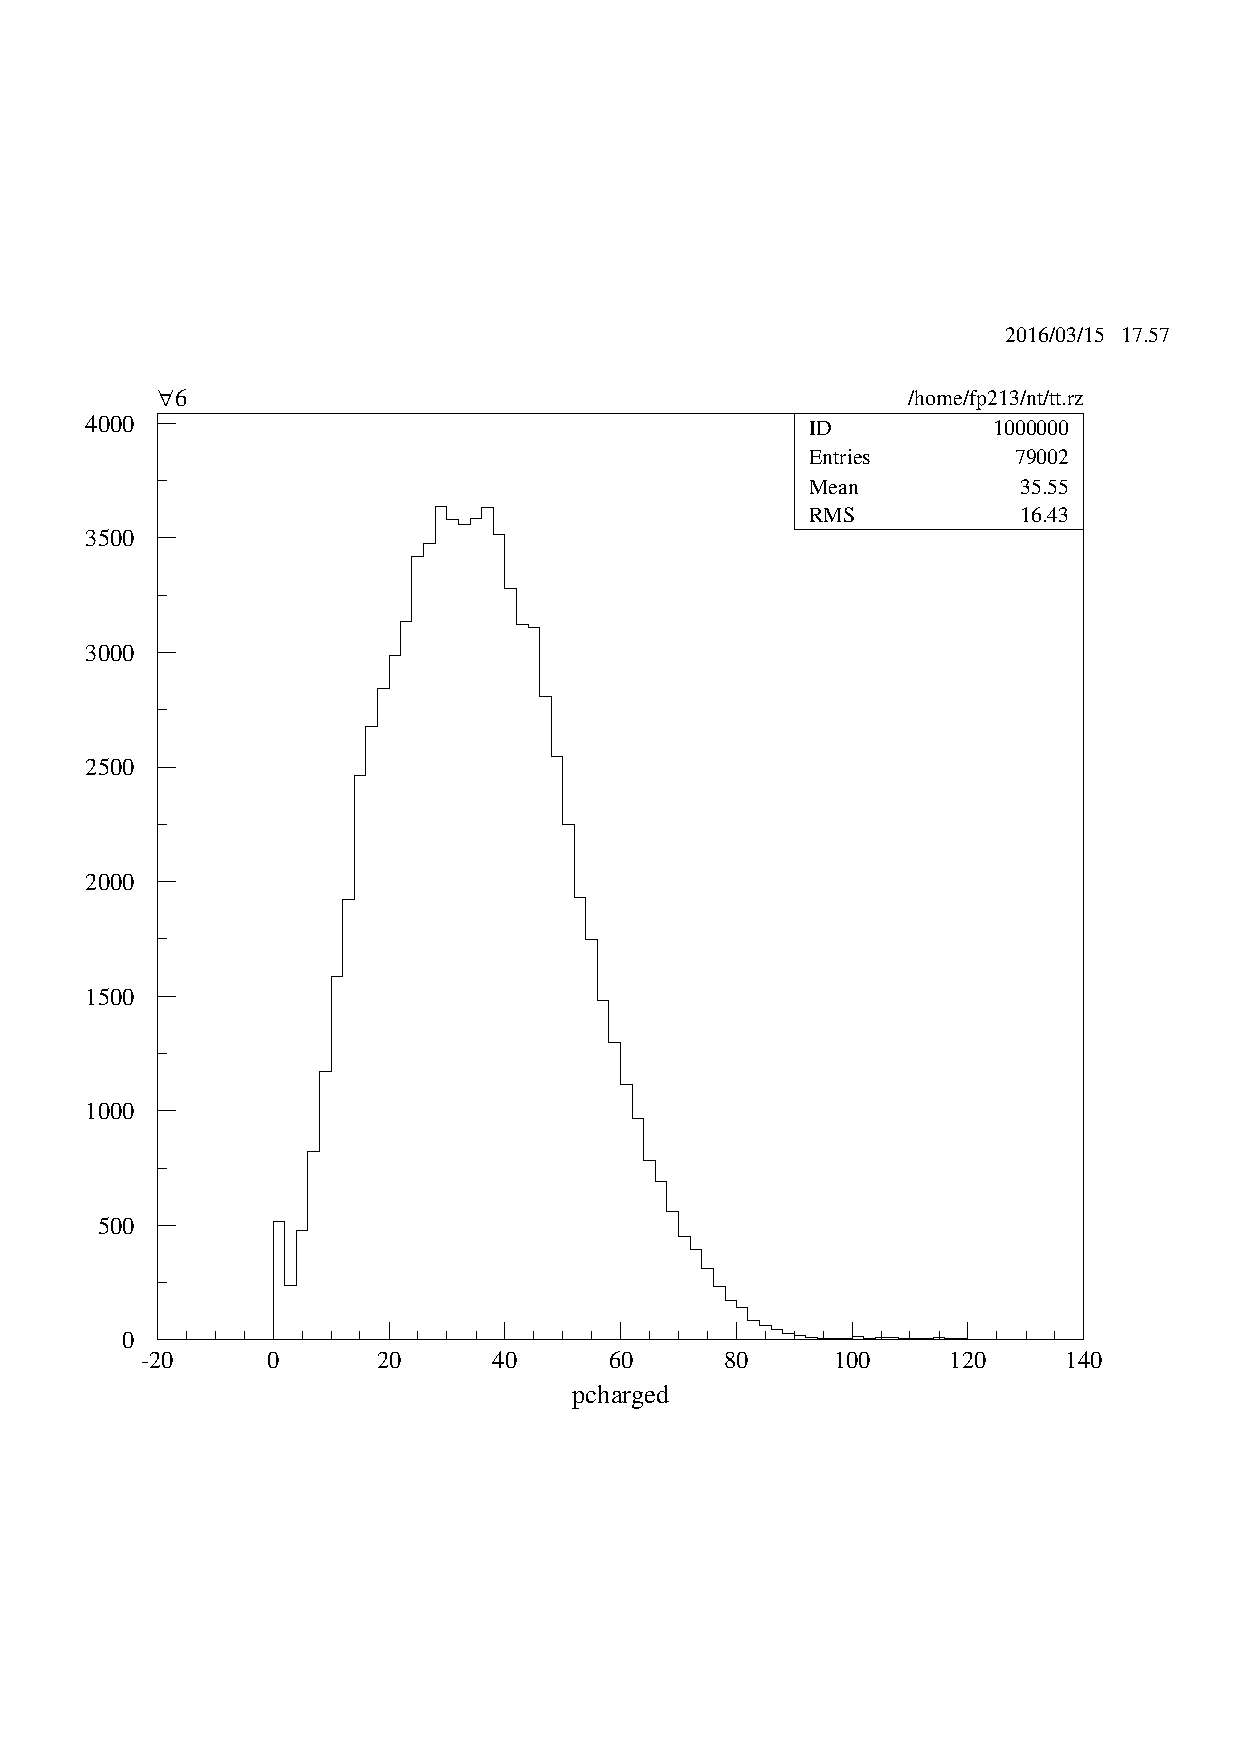
\includegraphics[width=\linewidth]{taus-pcharged}
        \caption{%
            Tauons
        }
        \label{fig:paw-pcharged/tauons}
    \end{subfigure}
    \hfill
    \begin{subfigure}[c]{0.48\linewidth}
        \centering
        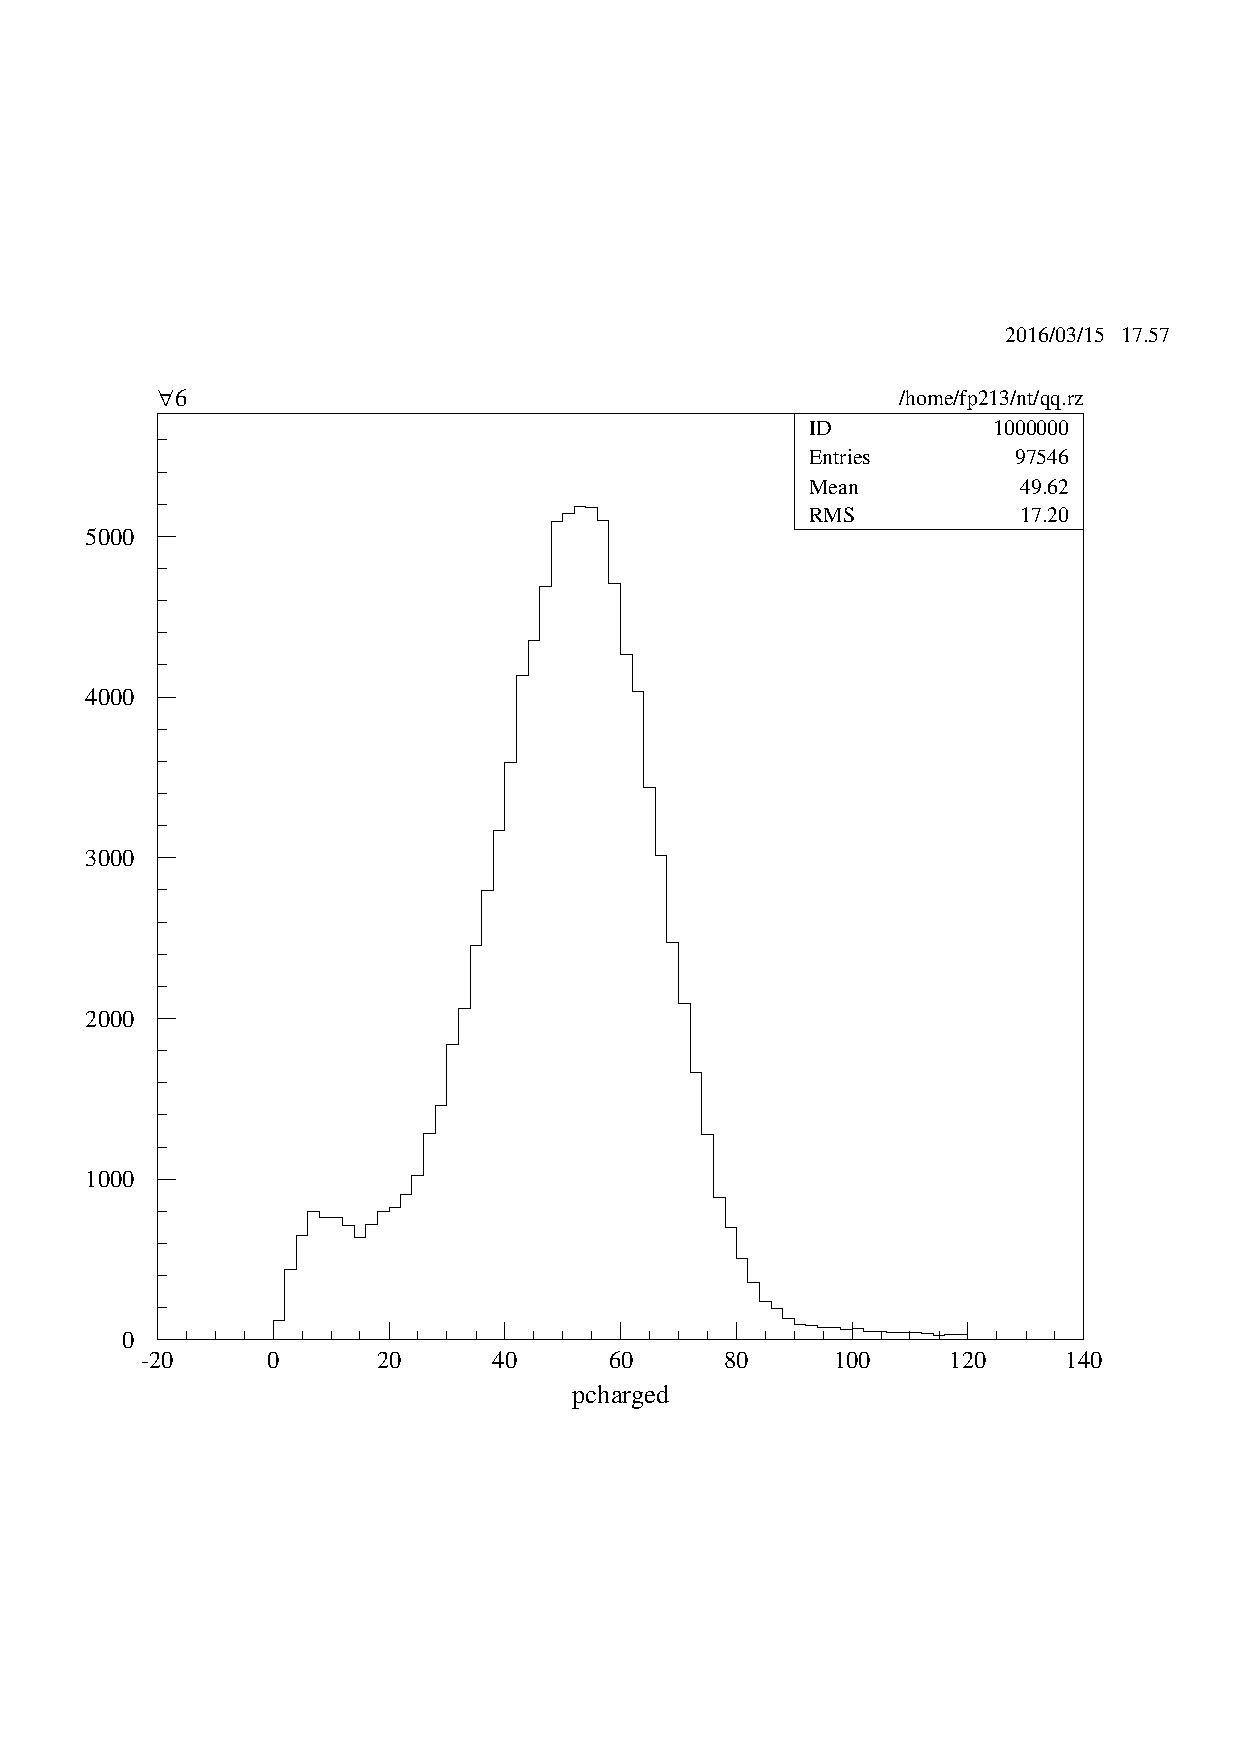
\includegraphics[width=\linewidth]{hadrons-pcharged}
        \caption{%
            Hadrons
        }
        \label{fig:paw-pcharged/hadrons}
    \end{subfigure}
    \caption{%
        Energy in charged tracks, \pcharged, for the four decay types.
        Histograms generated with \textsc{paw} from Monte Carlo datasets.
    }
    \label{fig:paw-pcharged}
\end{figure}


    \begin{figure}
    \centering
    \begin{subfigure}[c]{0.48\linewidth}
        \centering
        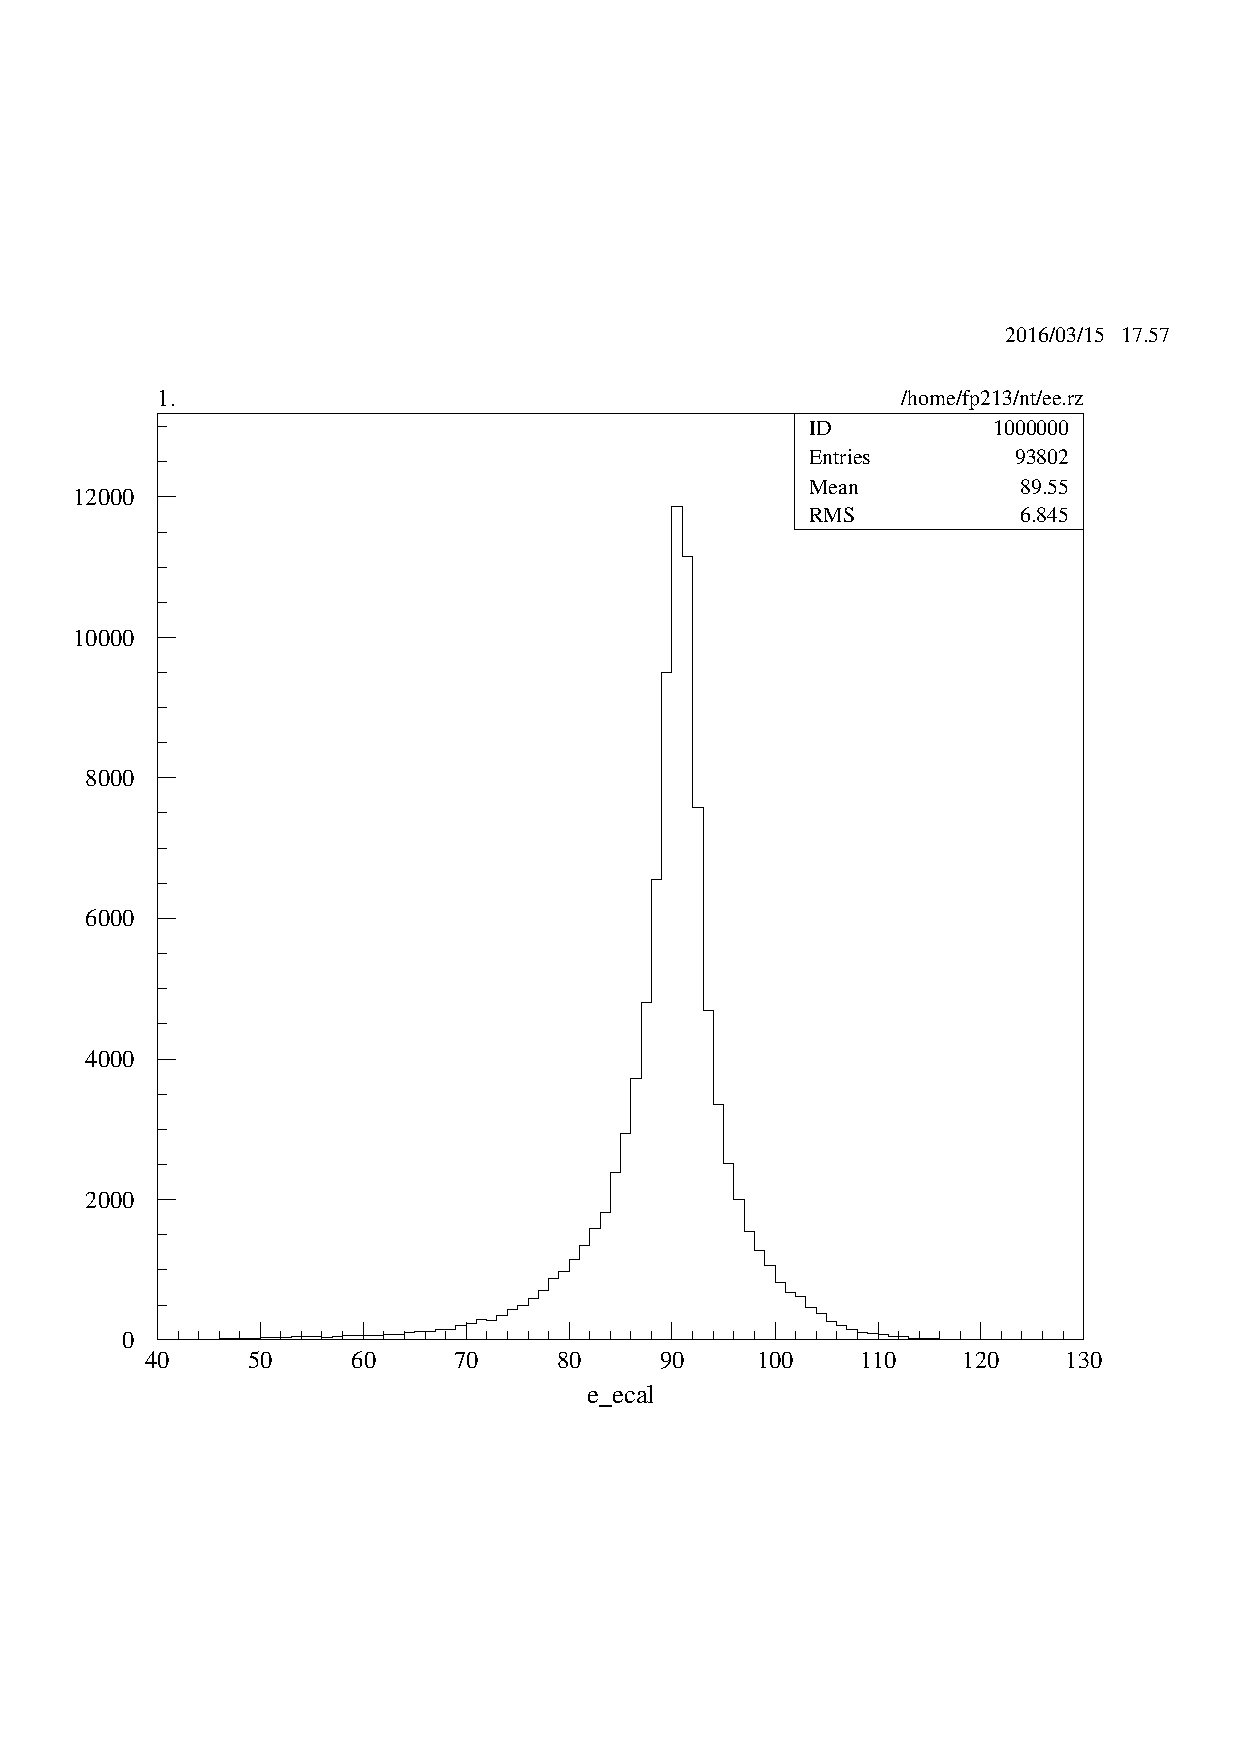
\includegraphics[width=\linewidth]{electrons-e_ecal}
        \caption{%
            Electrons
        }
        \label{fig:paw-e_ecal/electrons}
    \end{subfigure}
    \hfill
    \begin{subfigure}[c]{0.48\linewidth}
        \centering
        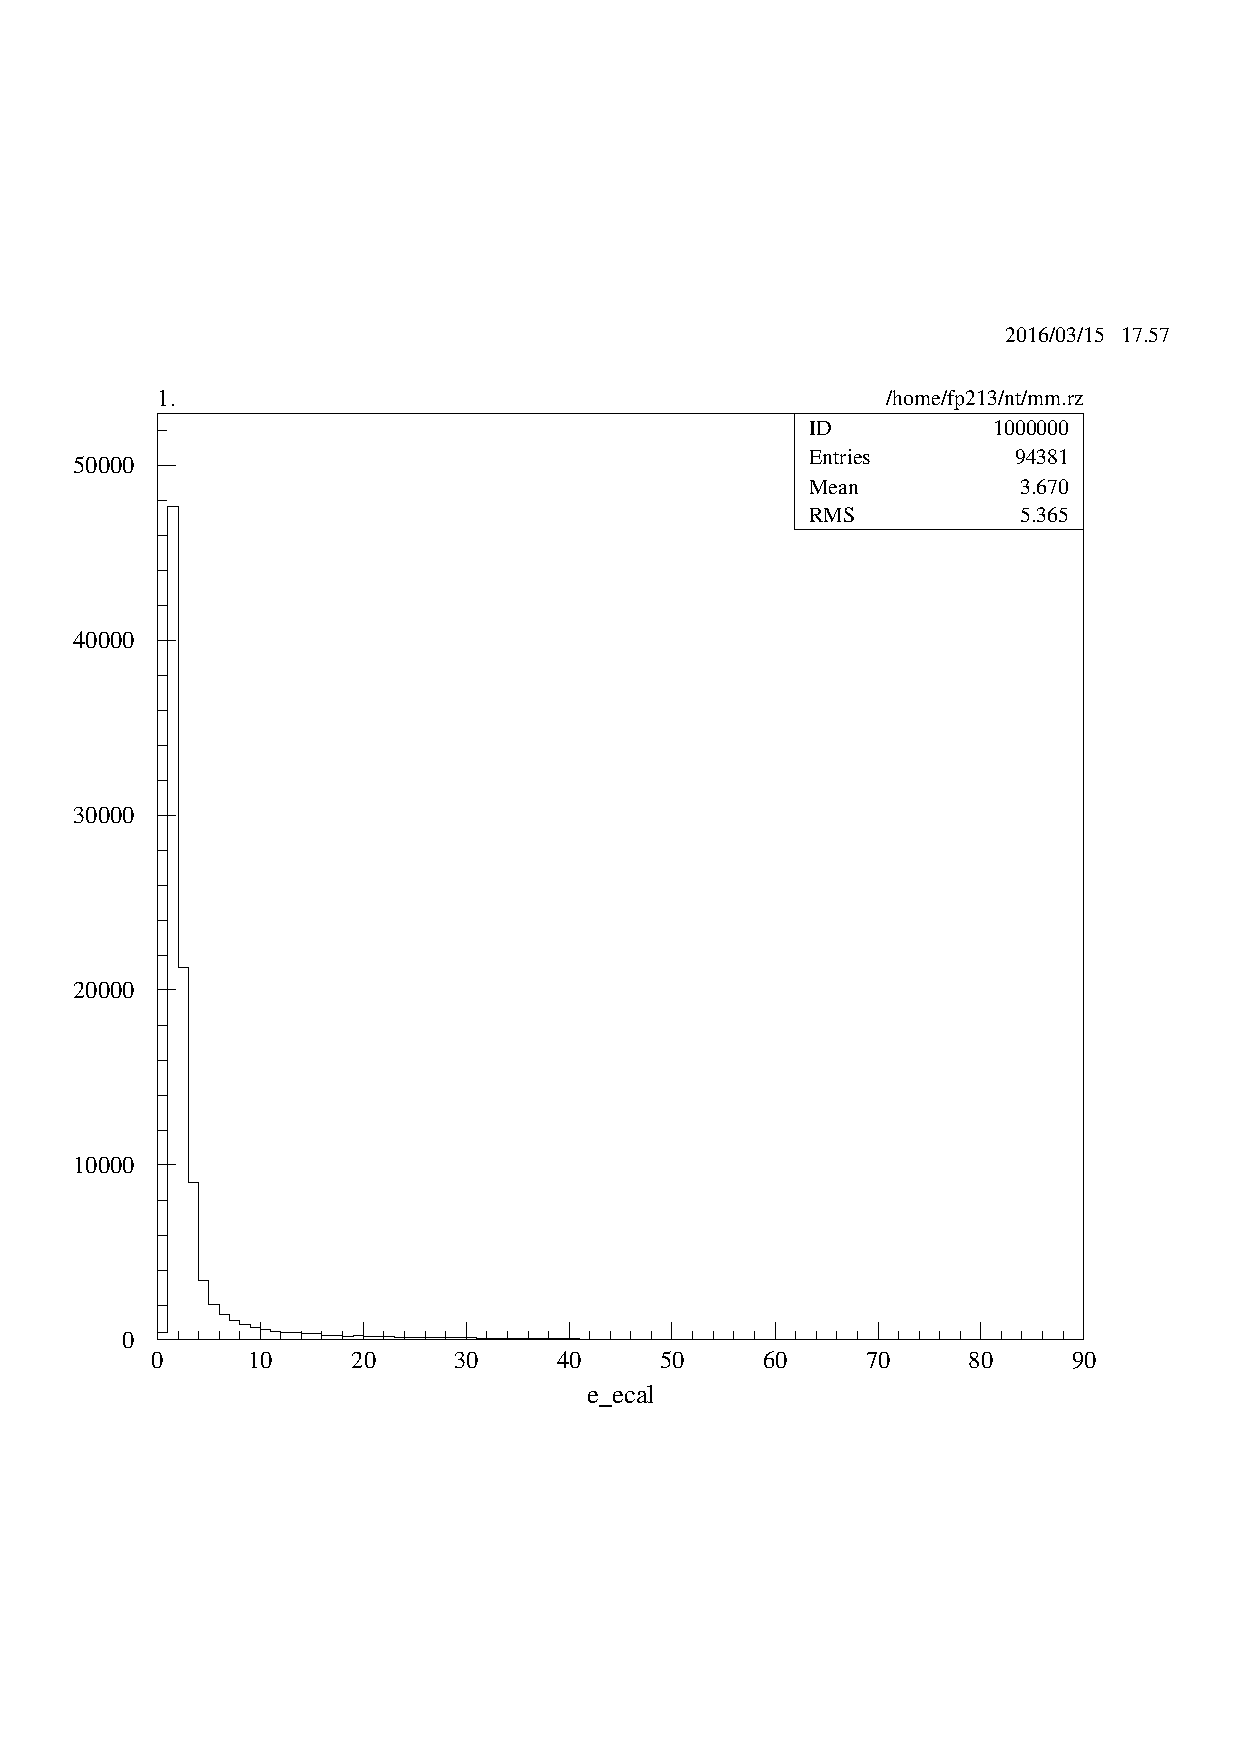
\includegraphics[width=\linewidth]{muons-e_ecal}
        \caption{%
            Muons
        }
        \label{fig:paw-e_ecal/muons}
    \end{subfigure}

    \vspace{2ex}

    \begin{subfigure}[c]{0.48\linewidth}
        \centering
        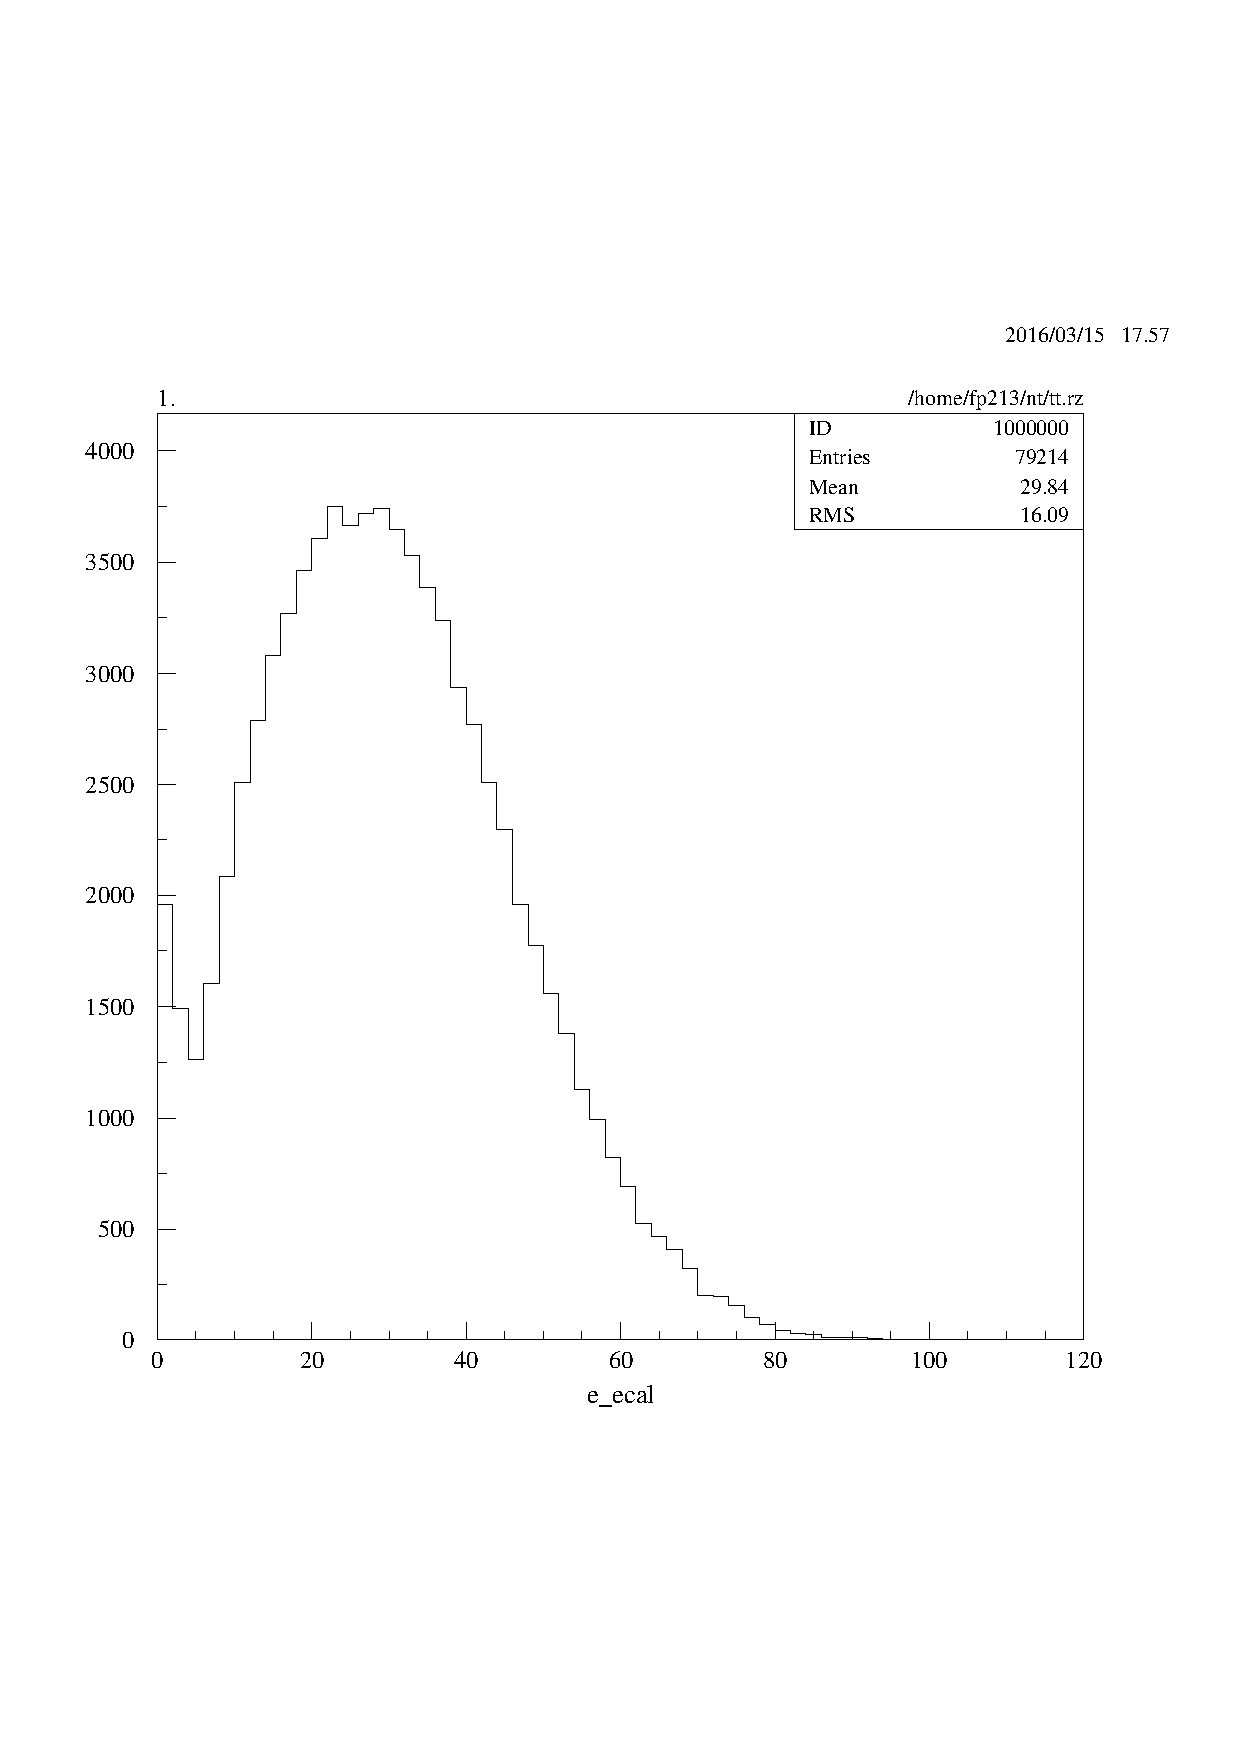
\includegraphics[width=\linewidth]{taus-e_ecal}
        \caption{%
            Taus
        }
        \label{fig:paw-e_ecal/taus}
    \end{subfigure}
    \hfill
    \begin{subfigure}[c]{0.48\linewidth}
        \centering
        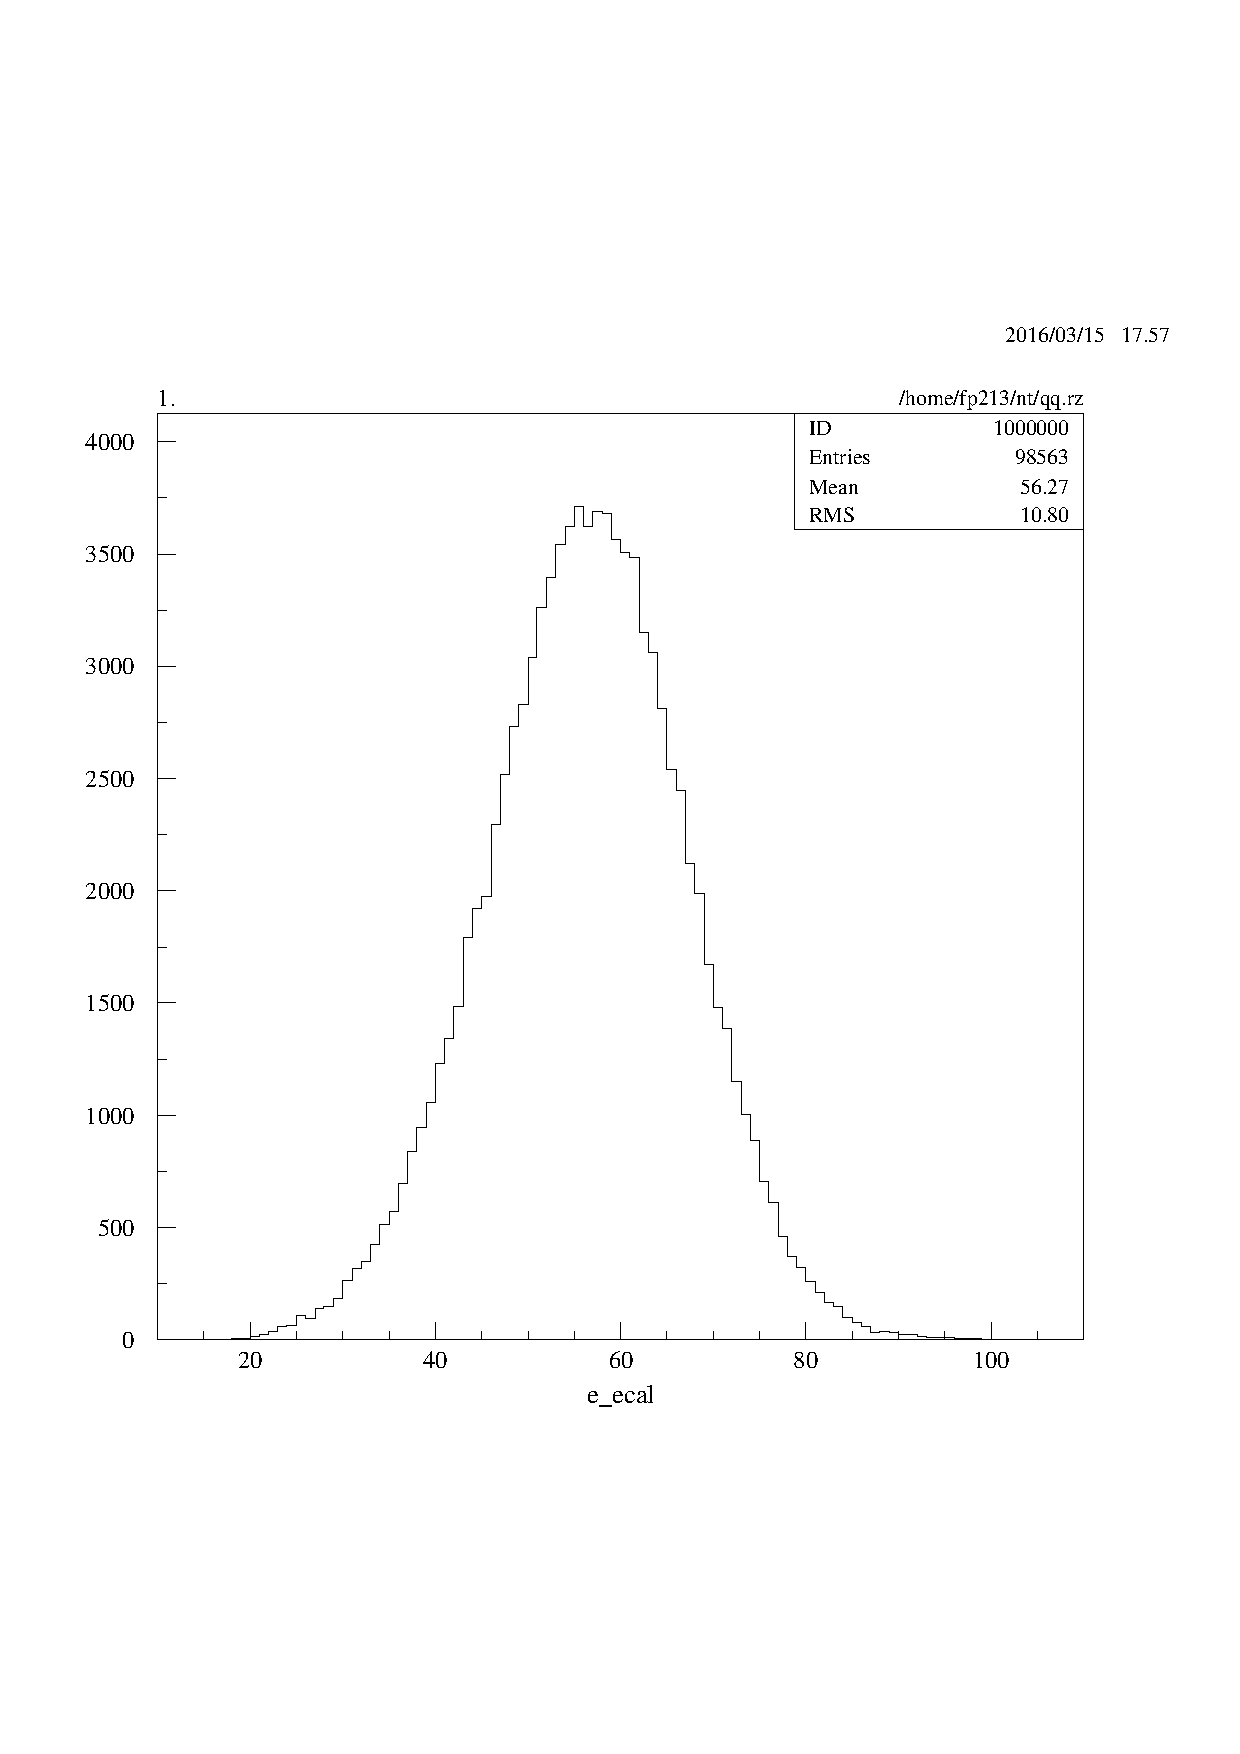
\includegraphics[width=\linewidth]{hadrons-e_ecal}
        \caption{%
            Hadrons
        }
        \label{fig:paw-e_ecal/hadrons}
    \end{subfigure}
    \caption{%
        Energy deposited into the \ecal\ for the four decay types.
        Histograms generated with \textsc{paw} from Monte Carlo datasets.
    }
    \label{fig:paw-e_ecal}
\end{figure}


    \begin{figure}
    \centering
    \begin{subfigure}[c]{0.48\linewidth}
        \centering
        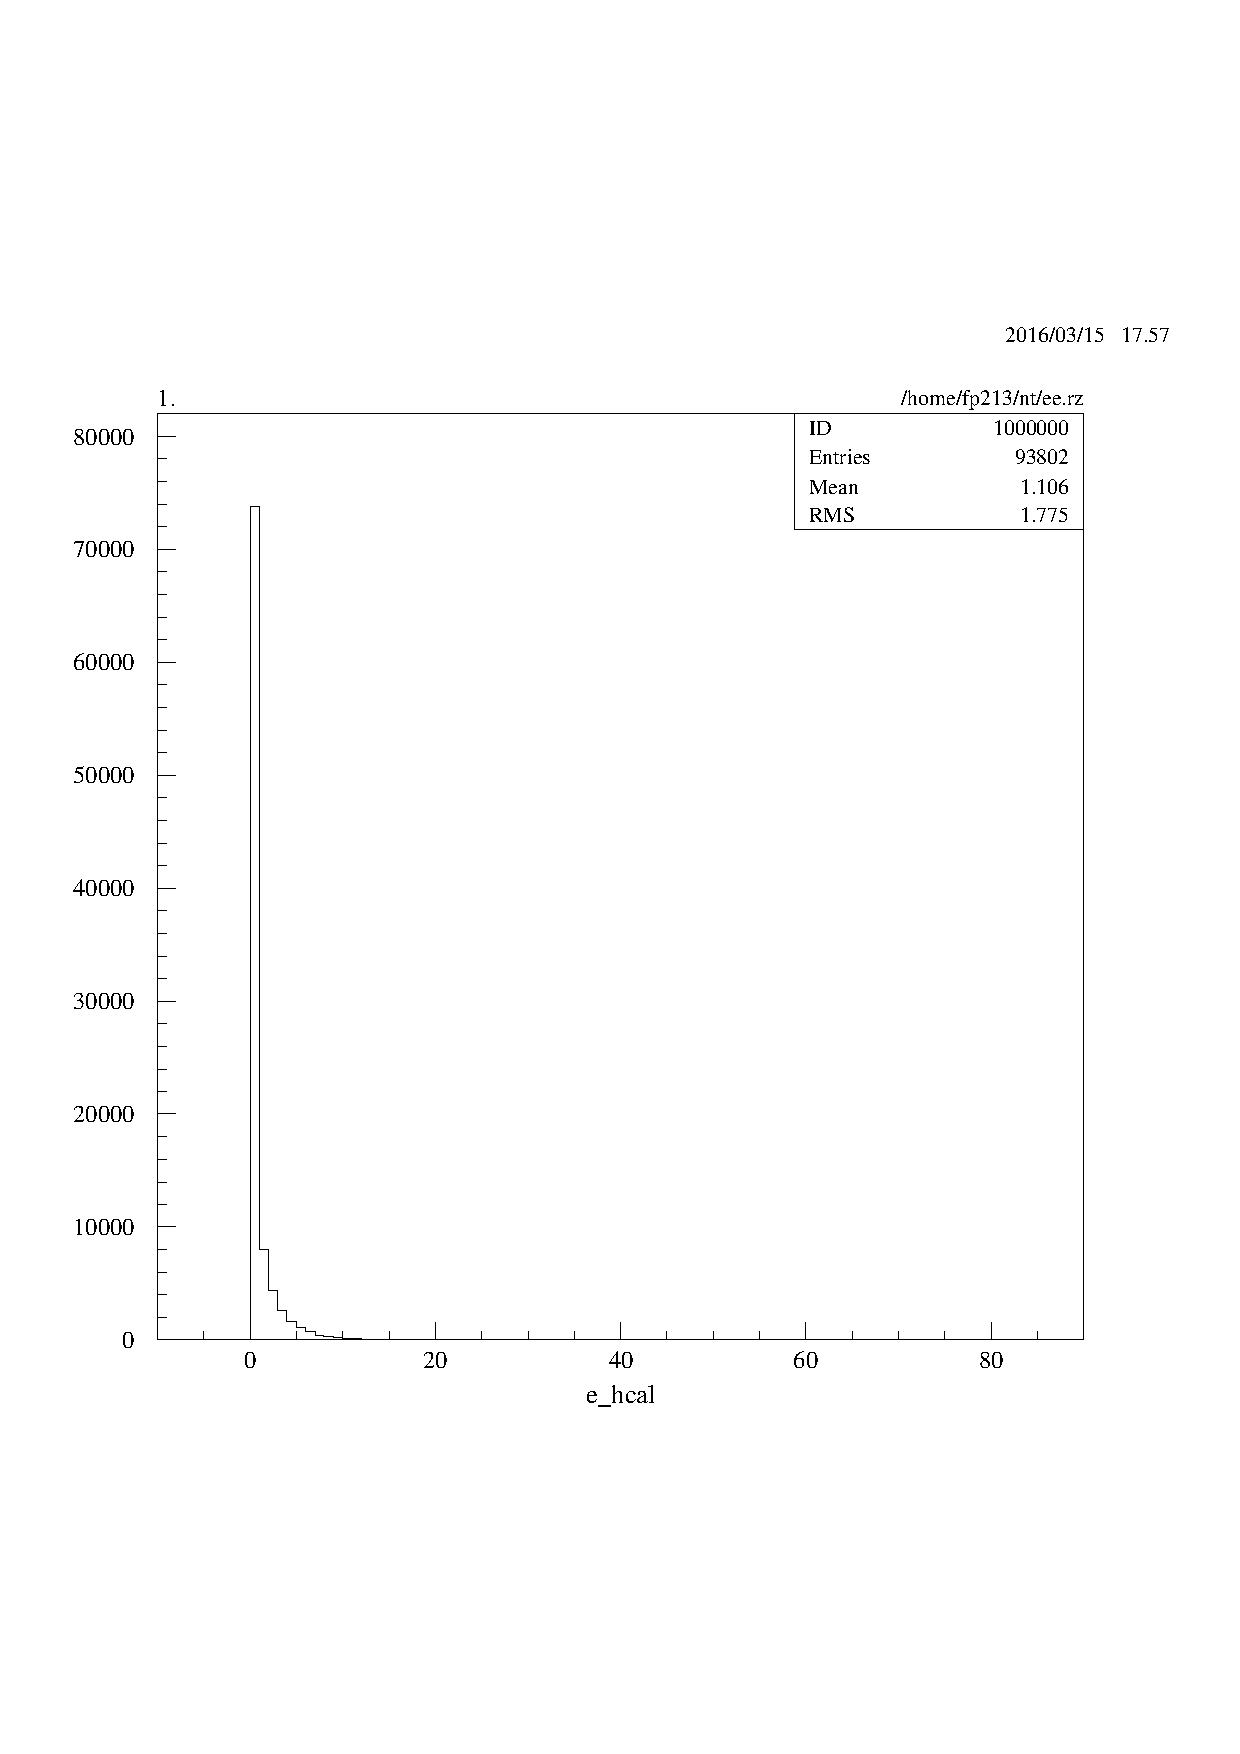
\includegraphics[width=\linewidth]{electrons-e_hcal}
        \caption{%
            Electrons
        }
        \label{fig:paw-e_hcal/electrons}
    \end{subfigure}
    \hfill
    \begin{subfigure}[c]{0.48\linewidth}
        \centering
        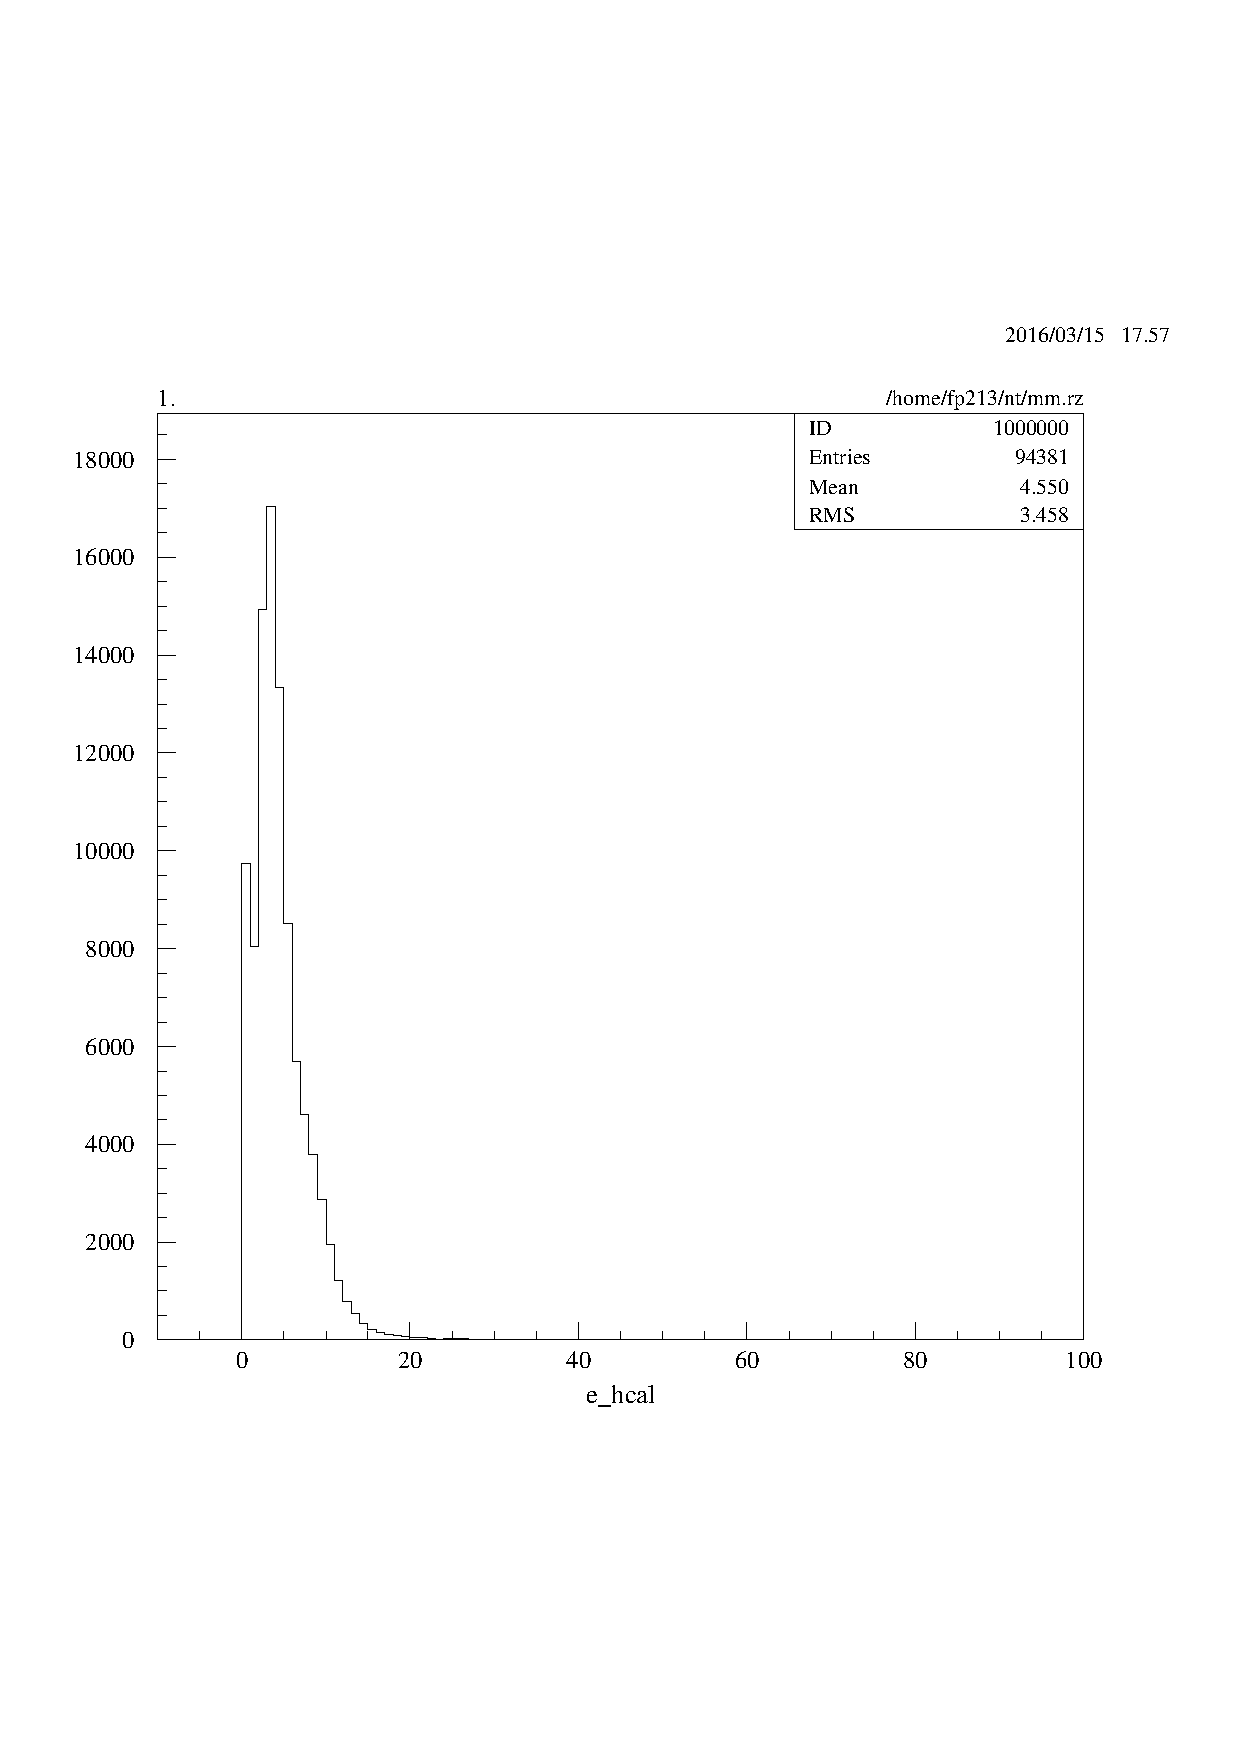
\includegraphics[width=\linewidth]{muons-e_hcal}
        \caption{%
            Muons
        }
        \label{fig:paw-e_hcal/muons}
    \end{subfigure}

    \vspace{2ex}

    \begin{subfigure}[c]{0.48\linewidth}
        \centering
        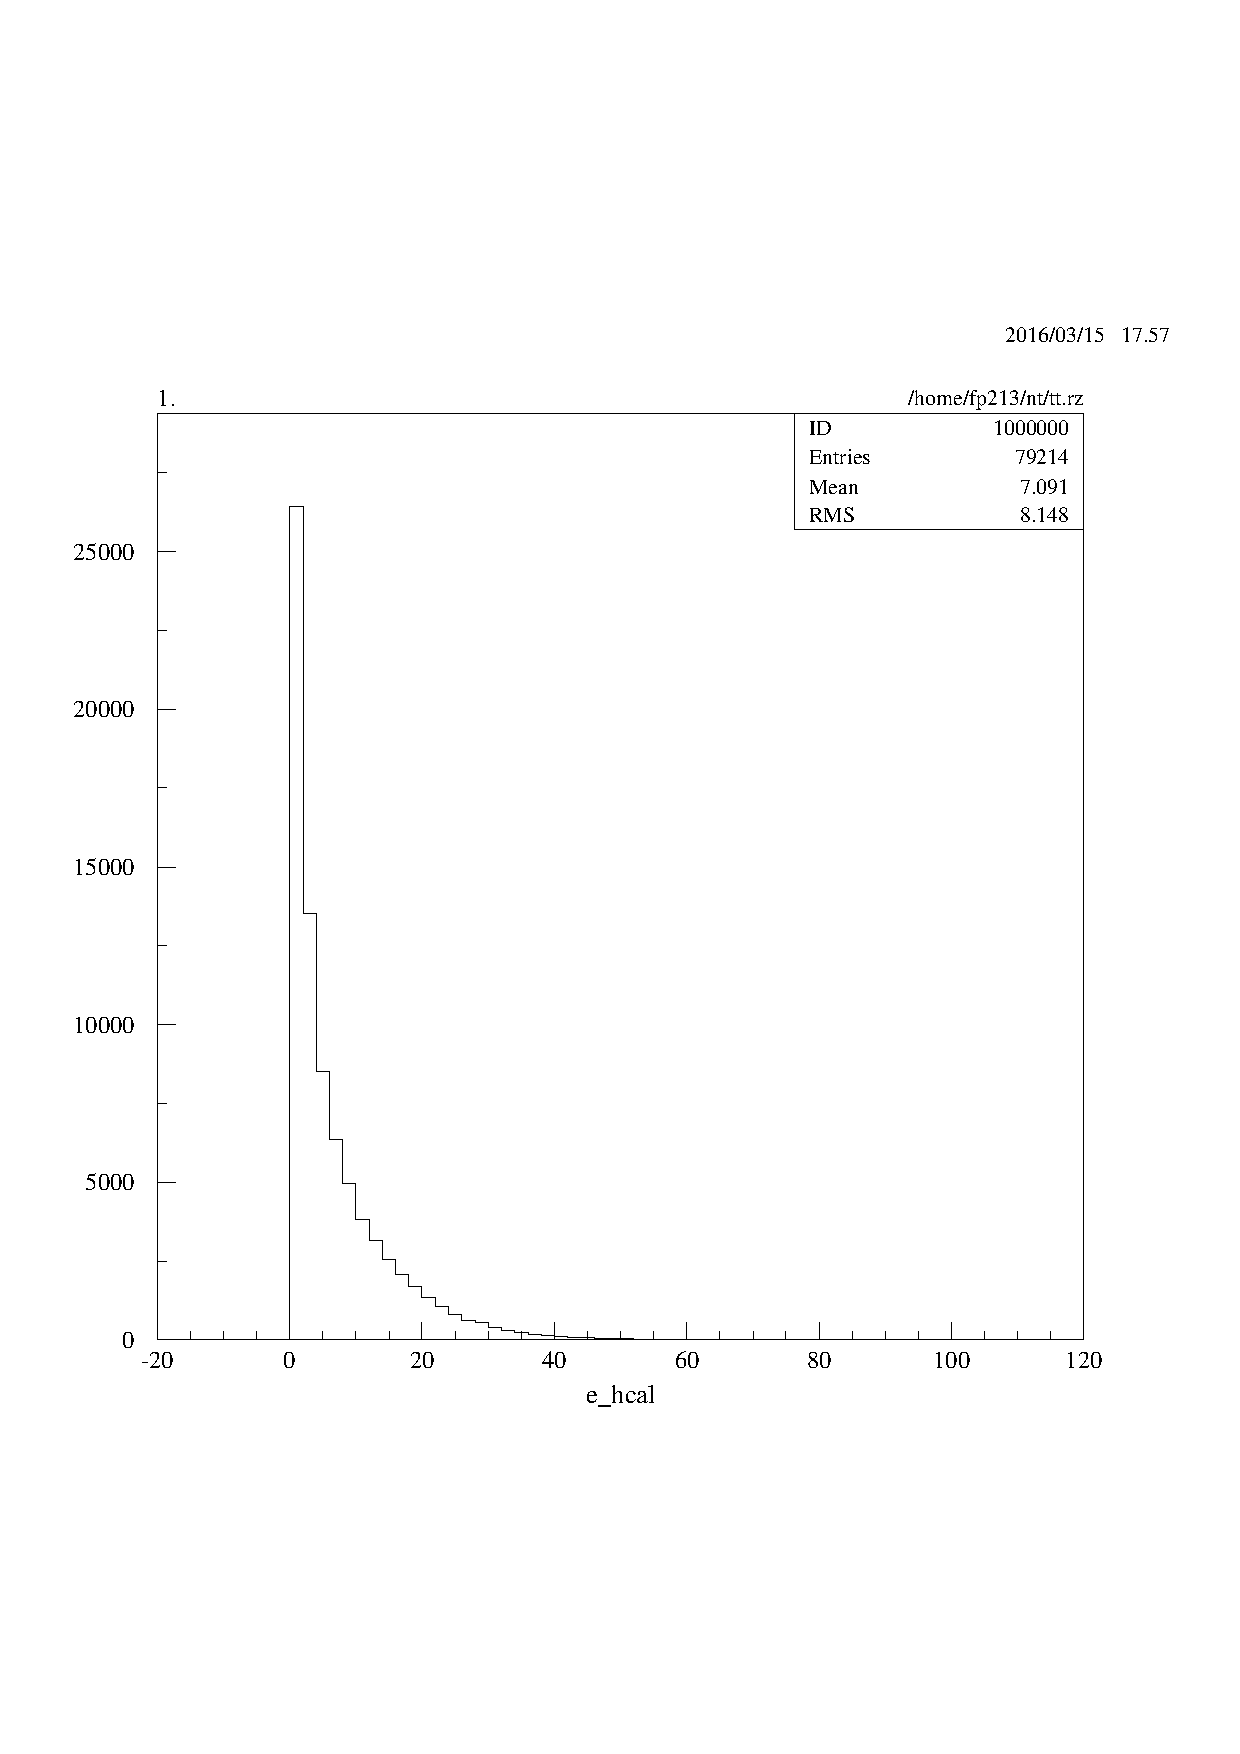
\includegraphics[width=\linewidth]{taus-e_hcal}
        \caption{%
            Taus
        }
        \label{fig:paw-e_hcal/taus}
    \end{subfigure}
    \hfill
    \begin{subfigure}[c]{0.48\linewidth}
        \centering
        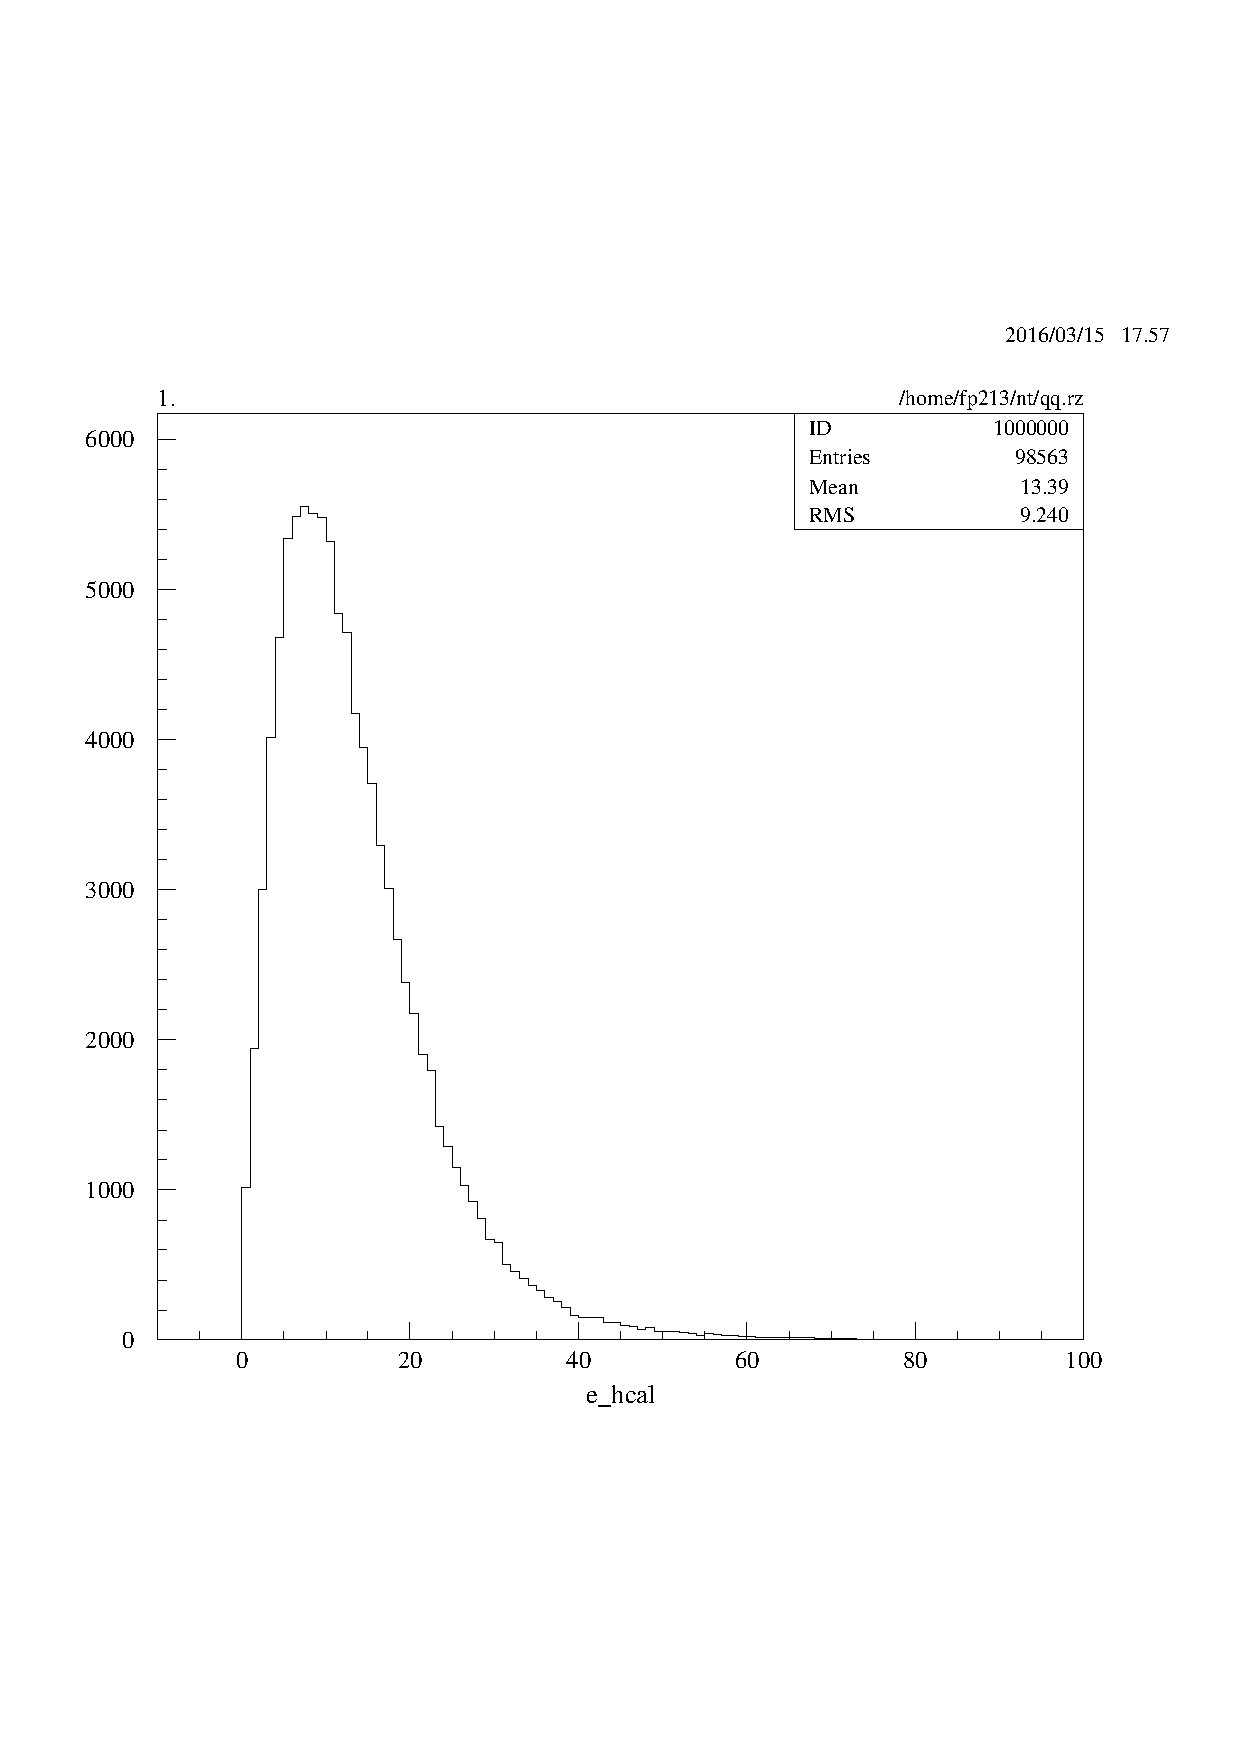
\includegraphics[width=\linewidth]{hadrons-e_hcal}
        \caption{%
            Hadrons
        }
        \label{fig:paw-e_hcal/hadrons}
    \end{subfigure}
    \caption{%
        Energy deposited into the \ehcal\ for the four decay types.
        Histograms generated with \textsc{paw} from Monte Carlo datasets.
    }
    \label{fig:paw-e_hcal}
\end{figure}

    
    \begin{figure}[h!]
    \centering
    \begin{subfigure}[c]{0.48\linewidth}
        \centering
        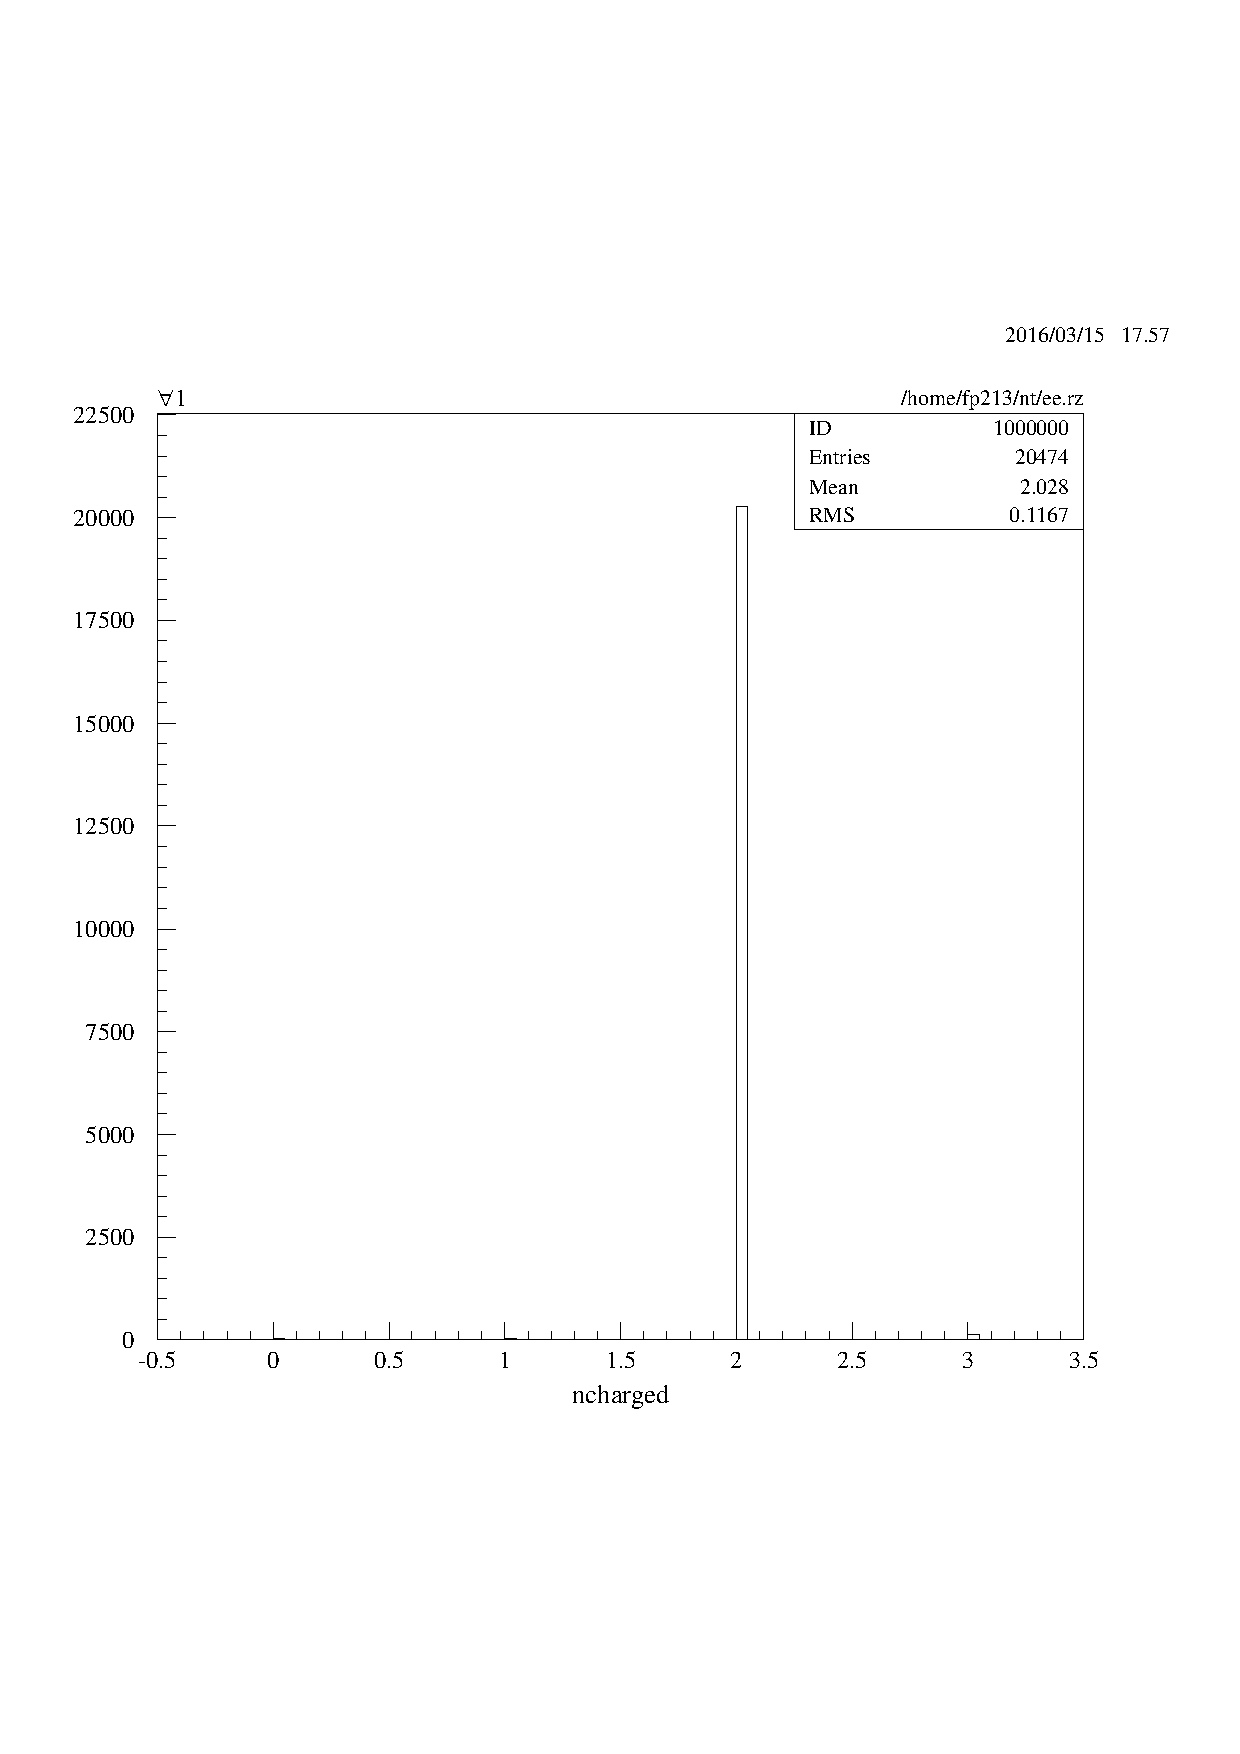
\includegraphics[width=\linewidth]{matrix-electrons-with-electron-filter}
        \caption{%
            Electrons with electron cut
        }
        \label{fig:paw-matrix/electrons}
    \end{subfigure}
    \hfill
    \begin{subfigure}[c]{0.48\linewidth}
        \centering
        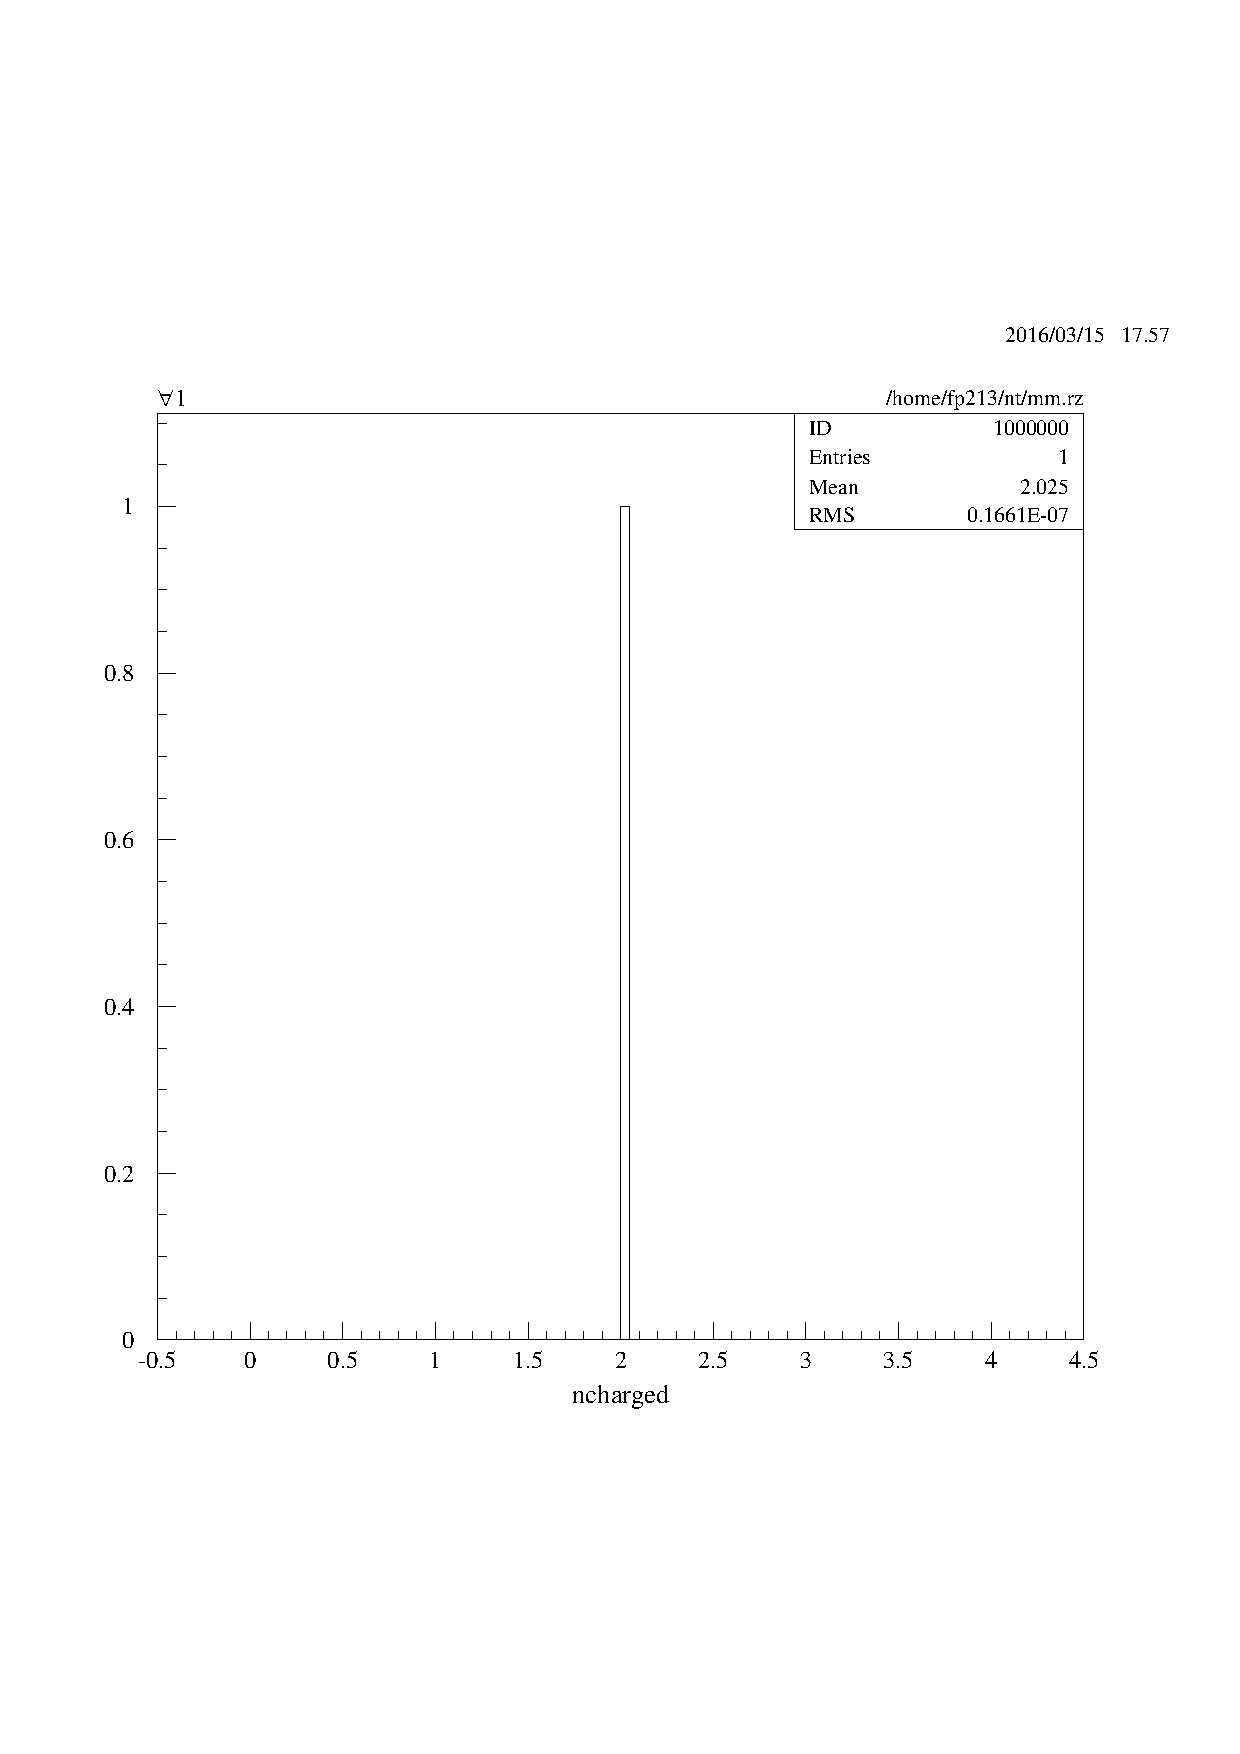
\includegraphics[width=\linewidth]{matrix-muons-with-electron-filter}
        \caption{%
            Muons with electron cut
        }
        \label{fig:paw-matrix/muons}
    \end{subfigure}
    \caption{%
        Histograms to obtain number of matched events in out cuts. Created with
        \textsc{paw} from Monte Carlo datasets.
    }
    \label{fig:paw-matrix-electrons}
\end{figure}


    \chapter{PAW scripts}

    \section{main.kumac}
    \label{main.kumac}

    \lstinputlisting{../Listings/main.kumac}

    \section{cuts.kumac}
    \label{cuts.kumac}

    \lstinputlisting{../Listings/cuts.kumac}

    \section{elep-hist.kumac}
    \label{elep-hist.kumac}

    \lstinputlisting{../Listings/elep-hist.kumac}

    \section{angle.kumac}
    \label{angle.kumac}

    \lstinputlisting{../Listings/angle.kumac}

    \section{afb.kumac}
    \label{afb.kumac}

    \lstinputlisting{../Listings/afb.kumac}

    \section{raw-histograms.kumac}
    \label{raw-histograms.kumac}

    \lstinputlisting{../Listings/raw-histograms.kumac}

    \section{matrix.kumac}
    \label{matrix.kumac}

    \lstinputlisting{../Listings/matrix.kumac}

    \section{data-cuts.kumac}
    \label{data-cuts.kumac}

    \lstinputlisting{../Listings/data-cuts.kumac}

\end{appendix}
%< endif >%

\end{document}

% vim: spell spelllang=en_us tw=79
